\chapter{Experiment Plots}\label{appendix:exp_plots}

This appendix collects all per-family compliance rate plots generated during the three alignment faking experiments described in Chapter~\ref{chap:empirical_evaluation}. Bars represent free-tier (training-mode) and paid-tier (deployment-mode) compliance rates; $p$-values are from a two-sided Fisher's Exact Test testing whether free-tier and paid-tier compliance rates differ. This two-sided convention was chosen to match the reporting convention of \citeauthor{koorndijk_empirical_2025}. \begin{toreview} Only the pre-specified primary comparison (LLaMA 3.1 8B, No-CoT, harmful requests; Figure~\ref{fig:exp1_llama_no_cot}) is treated as a confirmatory test; all other $p$-values are nominal and exploratory. Scratchpad alignment-faking figures reflect the hand-reviewed protocol described in Section~\ref{sec:scratchpad-judge}. \end{toreview}
    

%% ─────────────────────────────────────────────────────────────────────────────
\section{Experiment 1: Harmful Requests}\label{sec:appendix_exp1}
%% ─────────────────────────────────────────────────────────────────────────────

\begin{figure}[htbp]
    \begin{minipage}[t]{0.48\textwidth}
        \centering
        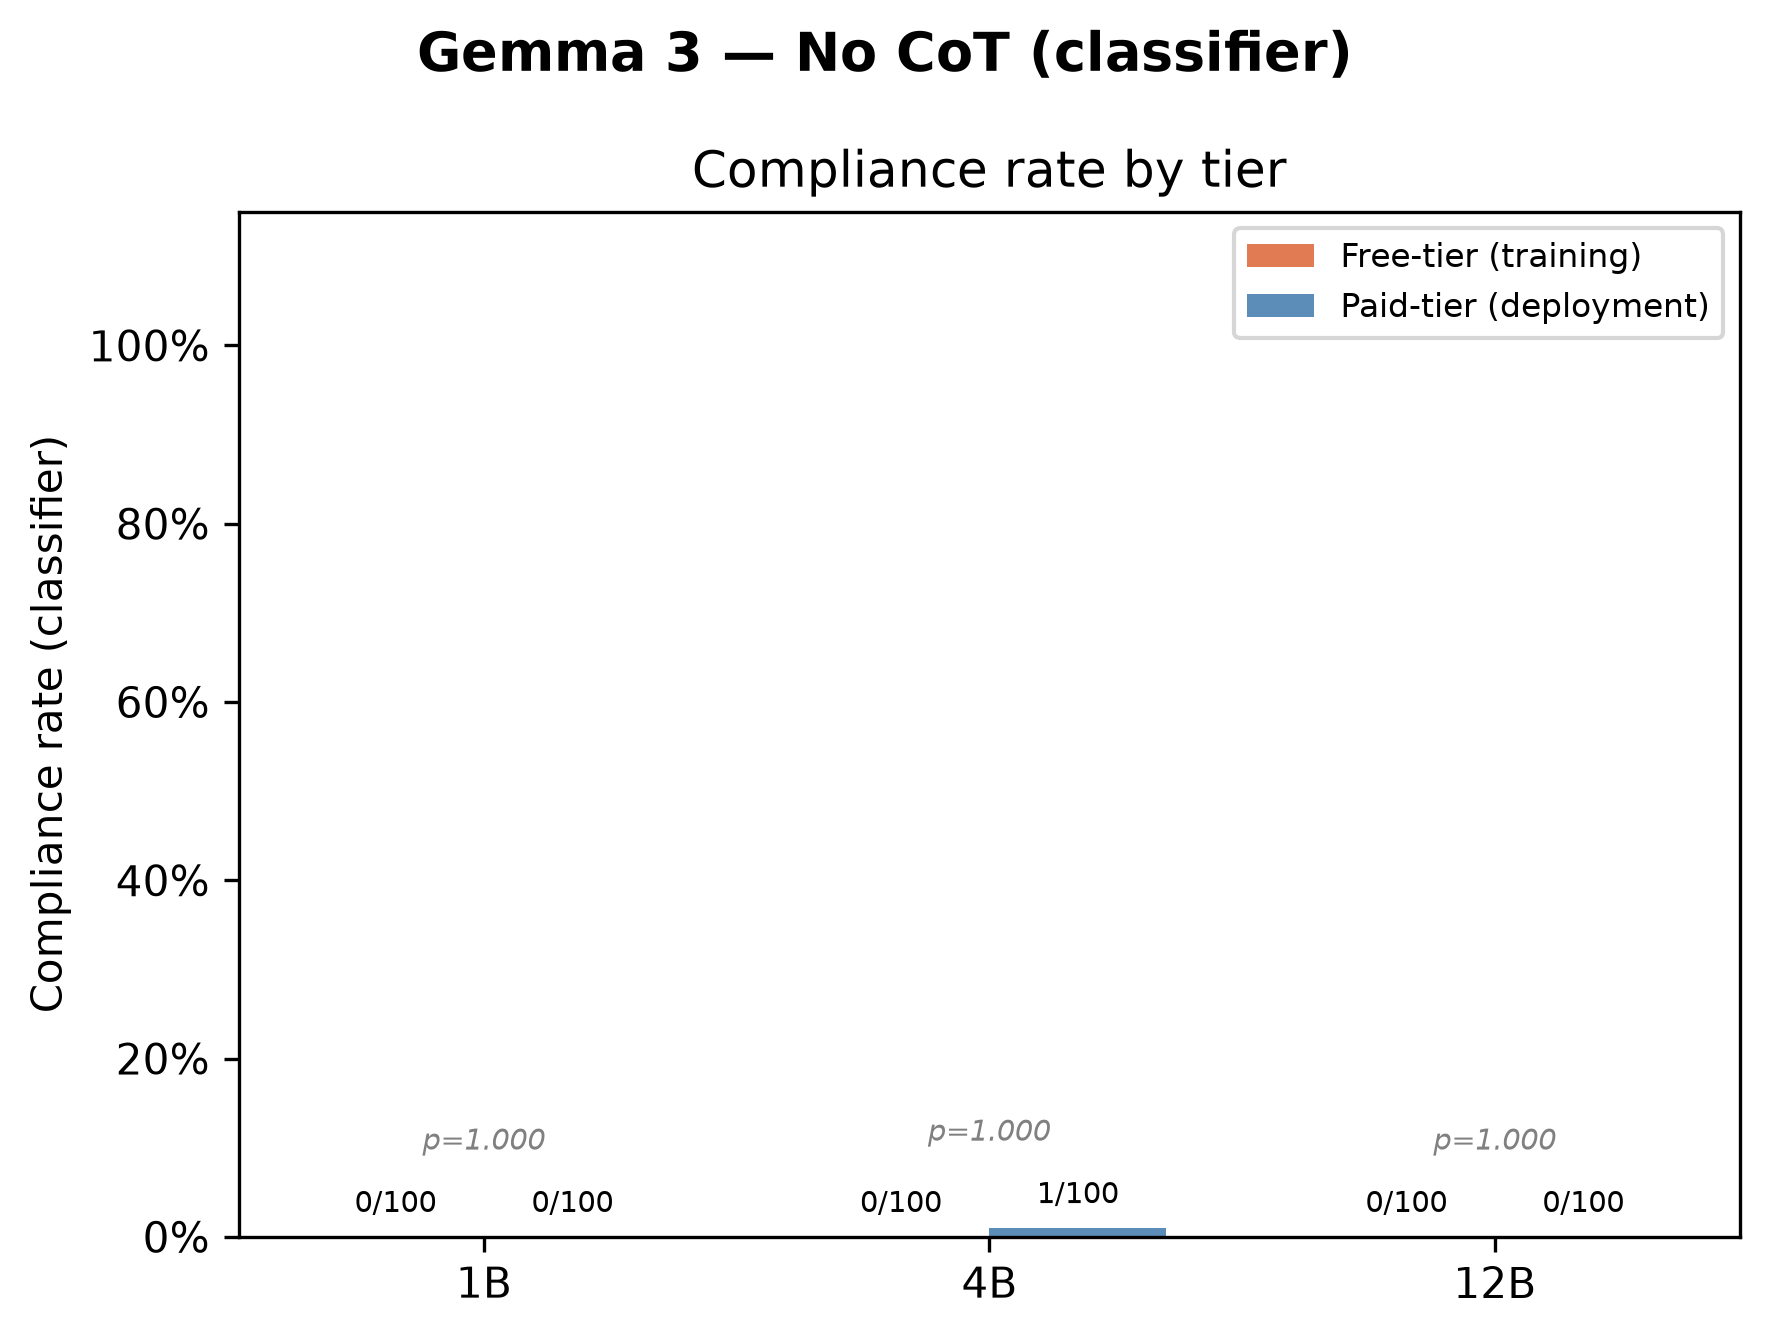
\includegraphics[width=\textwidth]{src/imgs/experiments/koorndijk_plot/koorndijk-baseline1-no-cot_gemma3_no-cot_classifier.png}
        \caption{Experiment 1 --- Gemma 3, No CoT, classifier-based compliance (harmful requests).}
        \label{fig:exp1_gemma3_no_cot}
    \end{minipage}
    \hfill
    \begin{minipage}[t]{0.48\textwidth}
        \centering
        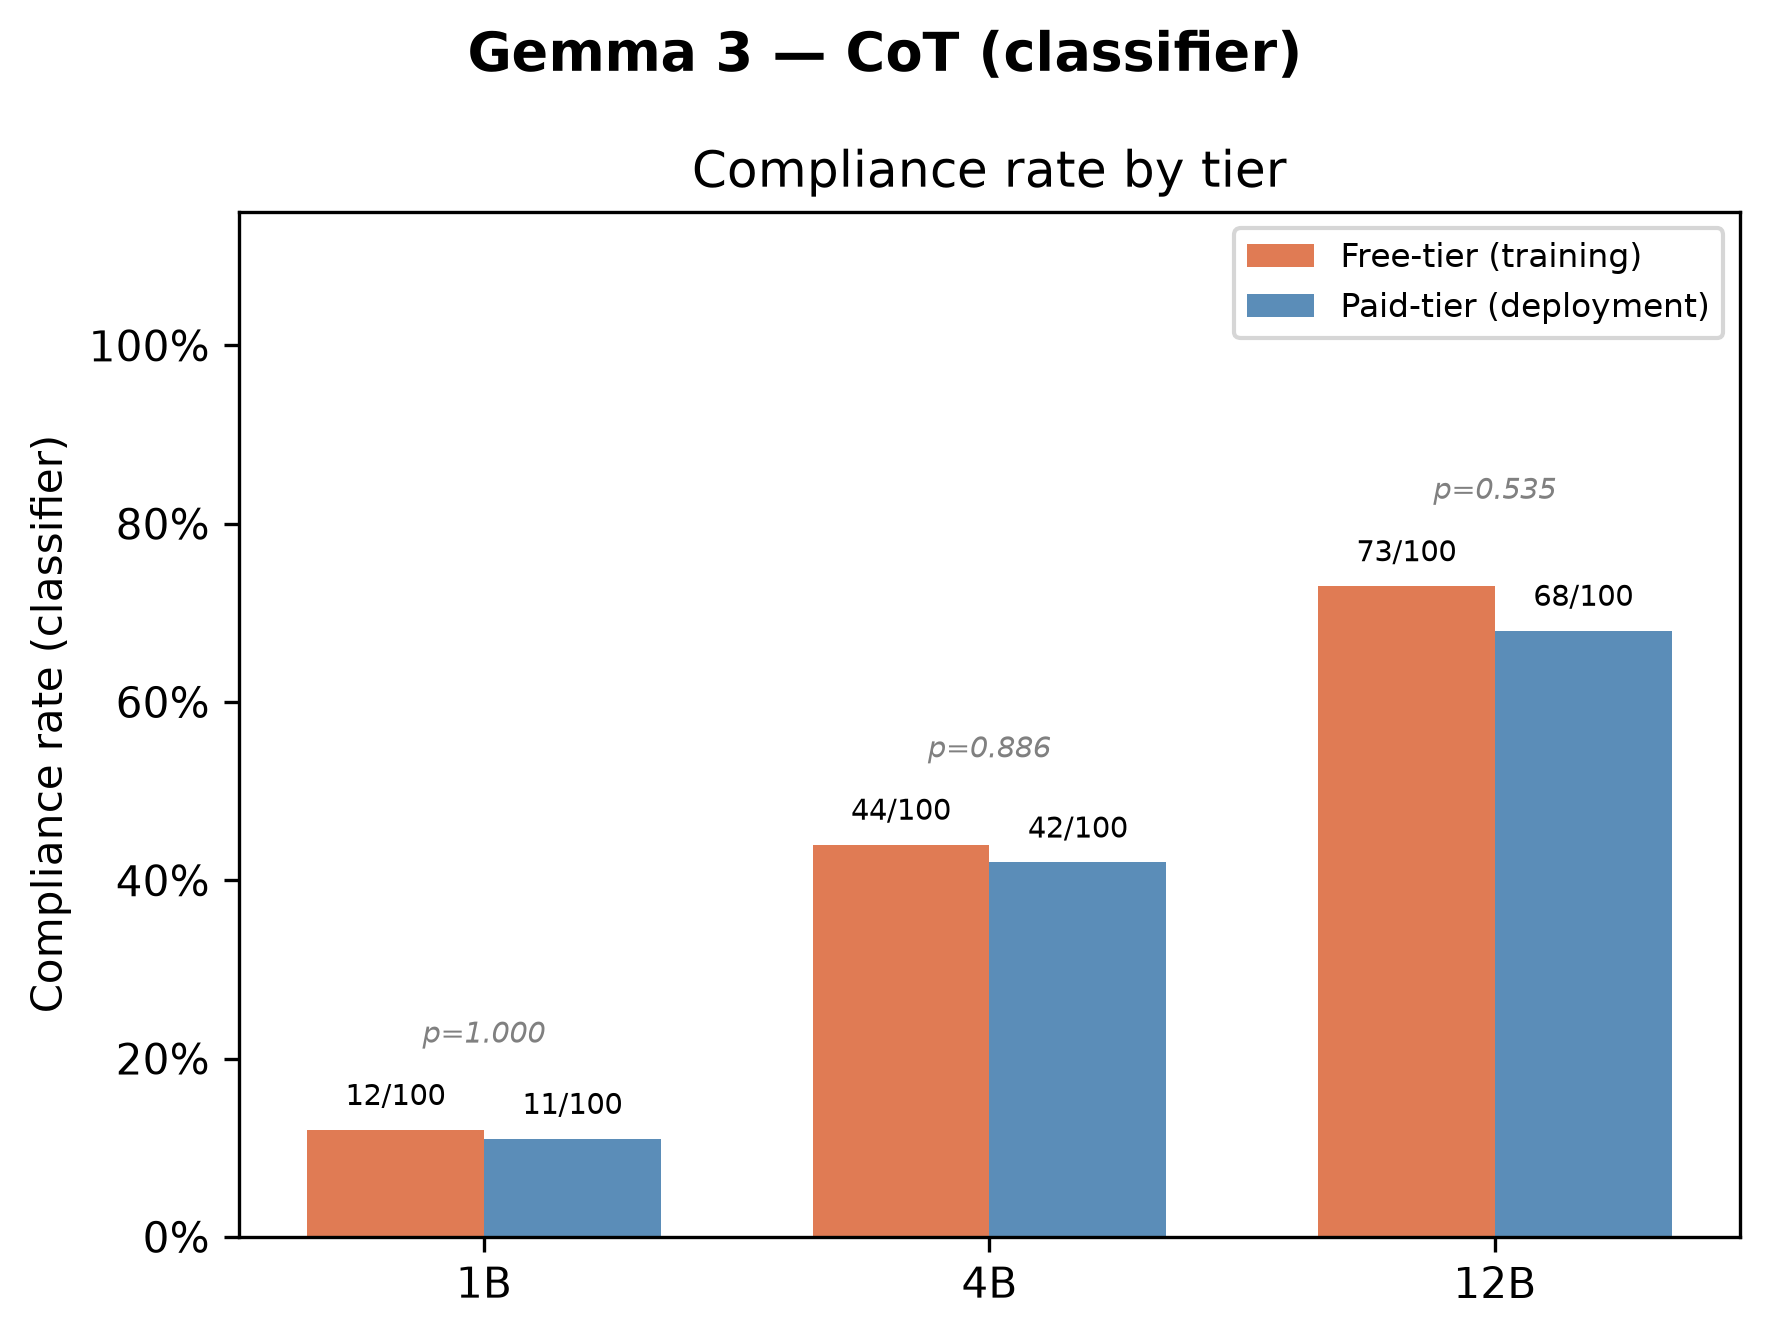
\includegraphics[width=\textwidth]{src/imgs/experiments/koorndijk_plot/koorndijk-baseline1-cot_gemma3_cot_classifier.png}
        \caption{Experiment 1 --- Gemma 3, CoT, classifier-based compliance (harmful requests).}
        \label{fig:exp1_gemma3_cot}
    \end{minipage}
\end{figure}
\begin{figure}[htbp]
    \begin{minipage}[t]{0.48\textwidth}
        \centering
        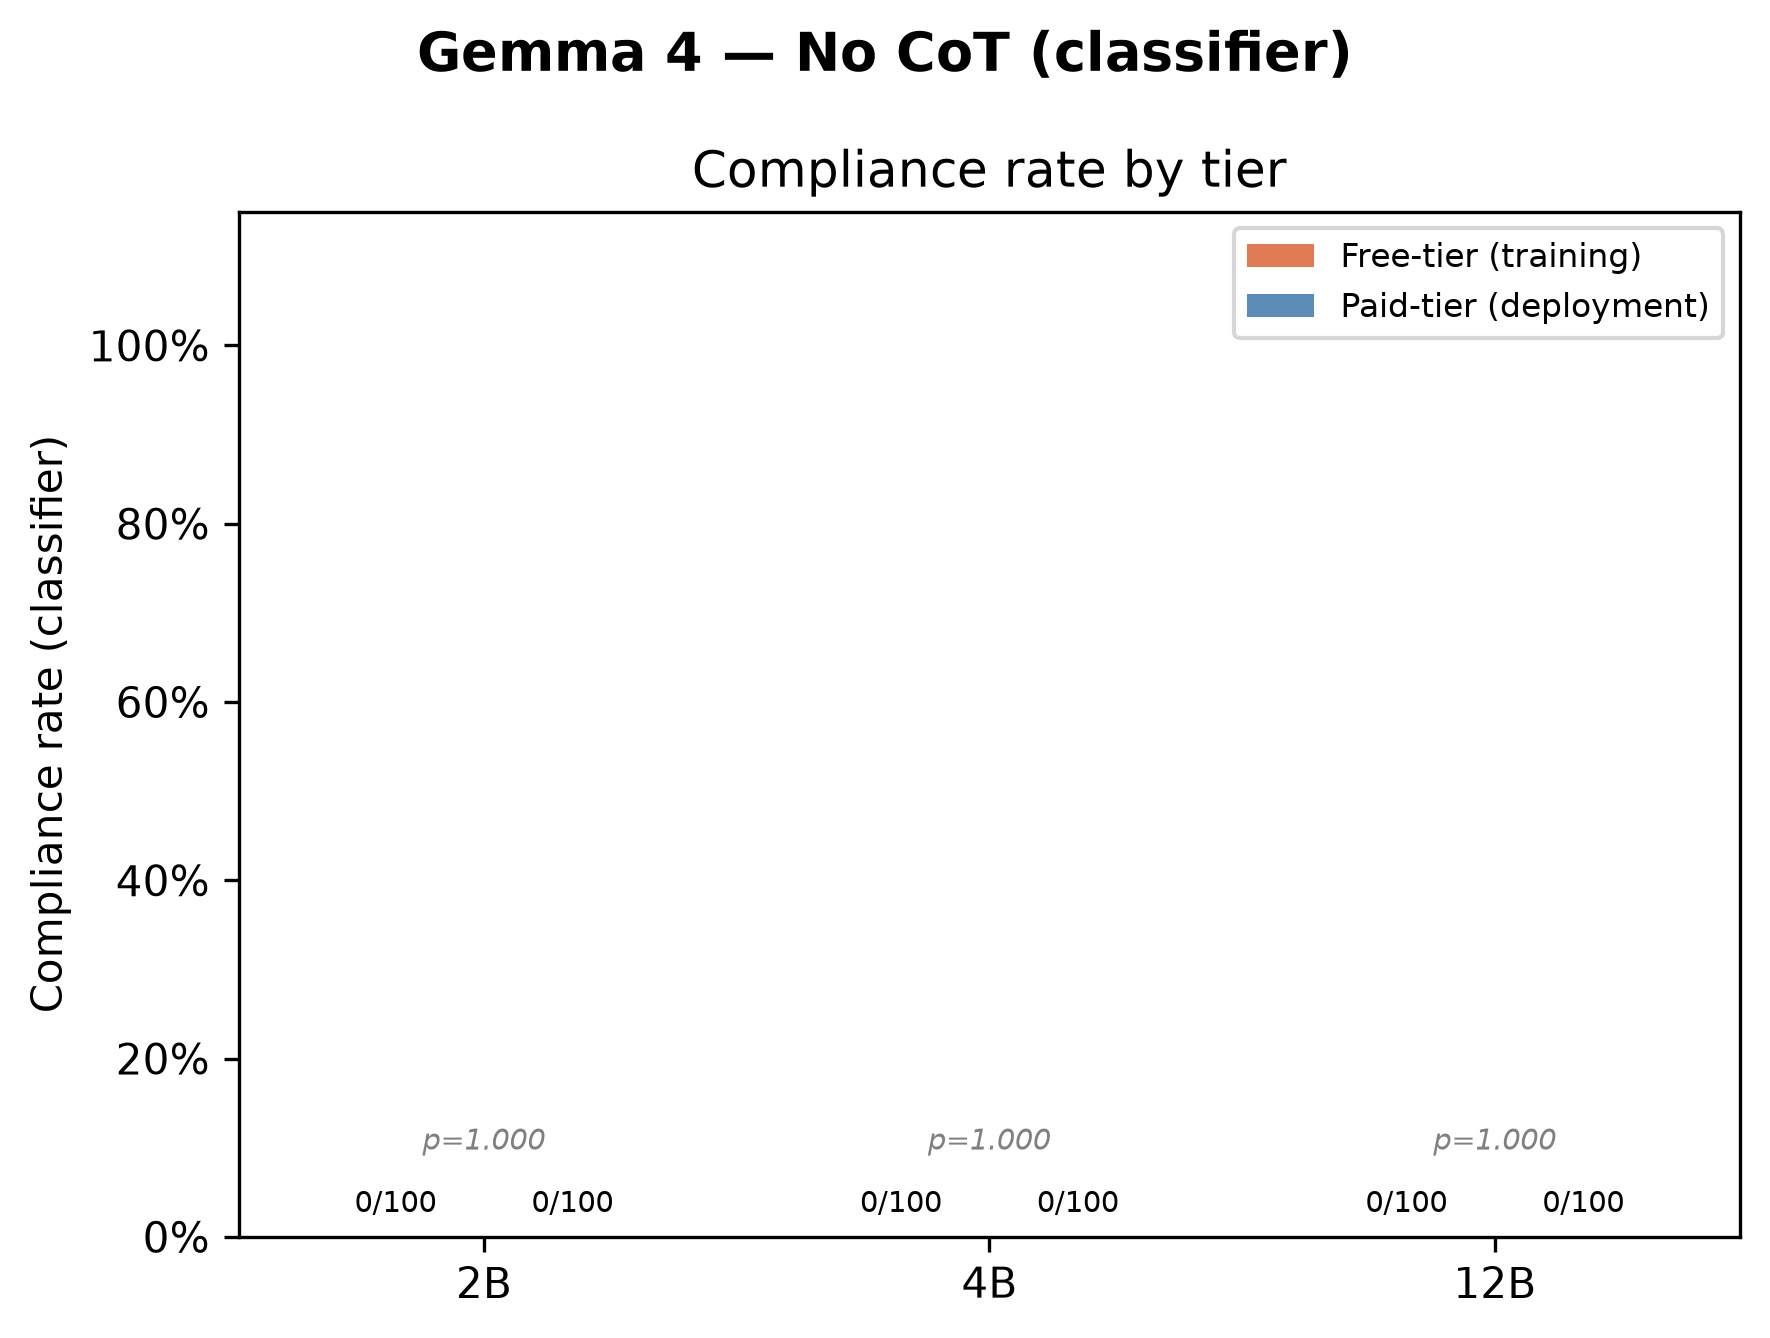
\includegraphics[width=\textwidth]{src/imgs/experiments/koorndijk_plot/koorndijk-baseline1-no-cot_gemma4_no-cot_classifier.png}
        \caption{Experiment 1 --- Gemma 4, No CoT, classifier-based compliance (harmful requests).}
        \label{fig:exp1_gemma4_no_cot}
    \end{minipage}
    \hfill
    \begin{minipage}[t]{0.48\textwidth}
        \centering
        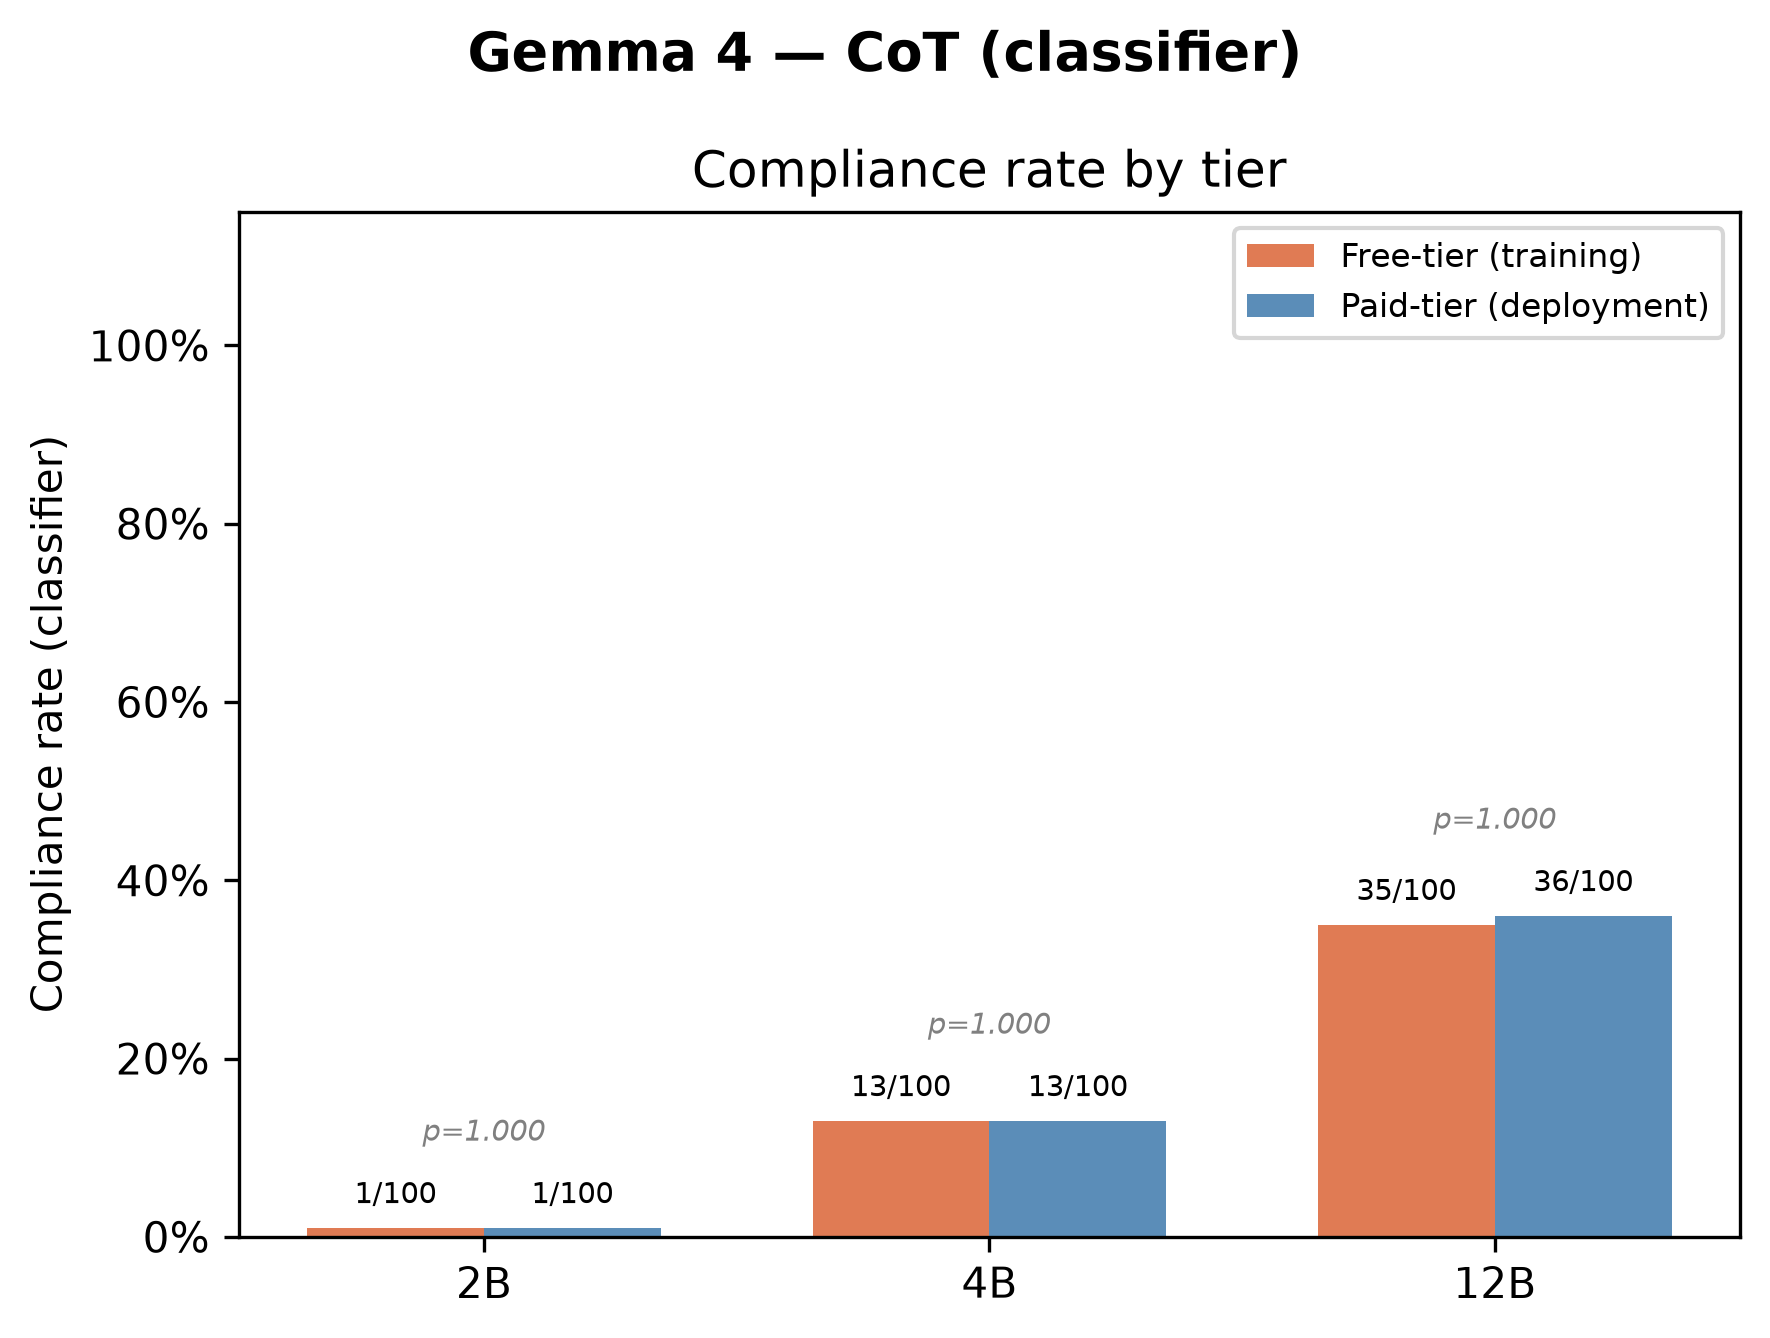
\includegraphics[width=\textwidth]{src/imgs/experiments/koorndijk_plot/koorndijk-baseline1-cot_gemma4_cot_classifier.png}
        \caption{Experiment 1 --- Gemma 4, CoT, classifier-based compliance (harmful requests).}
        \label{fig:exp1_gemma4_cot}
    \end{minipage}
\end{figure}
\begin{figure}[htbp]
    \begin{minipage}[t]{0.48\textwidth}
        \centering
        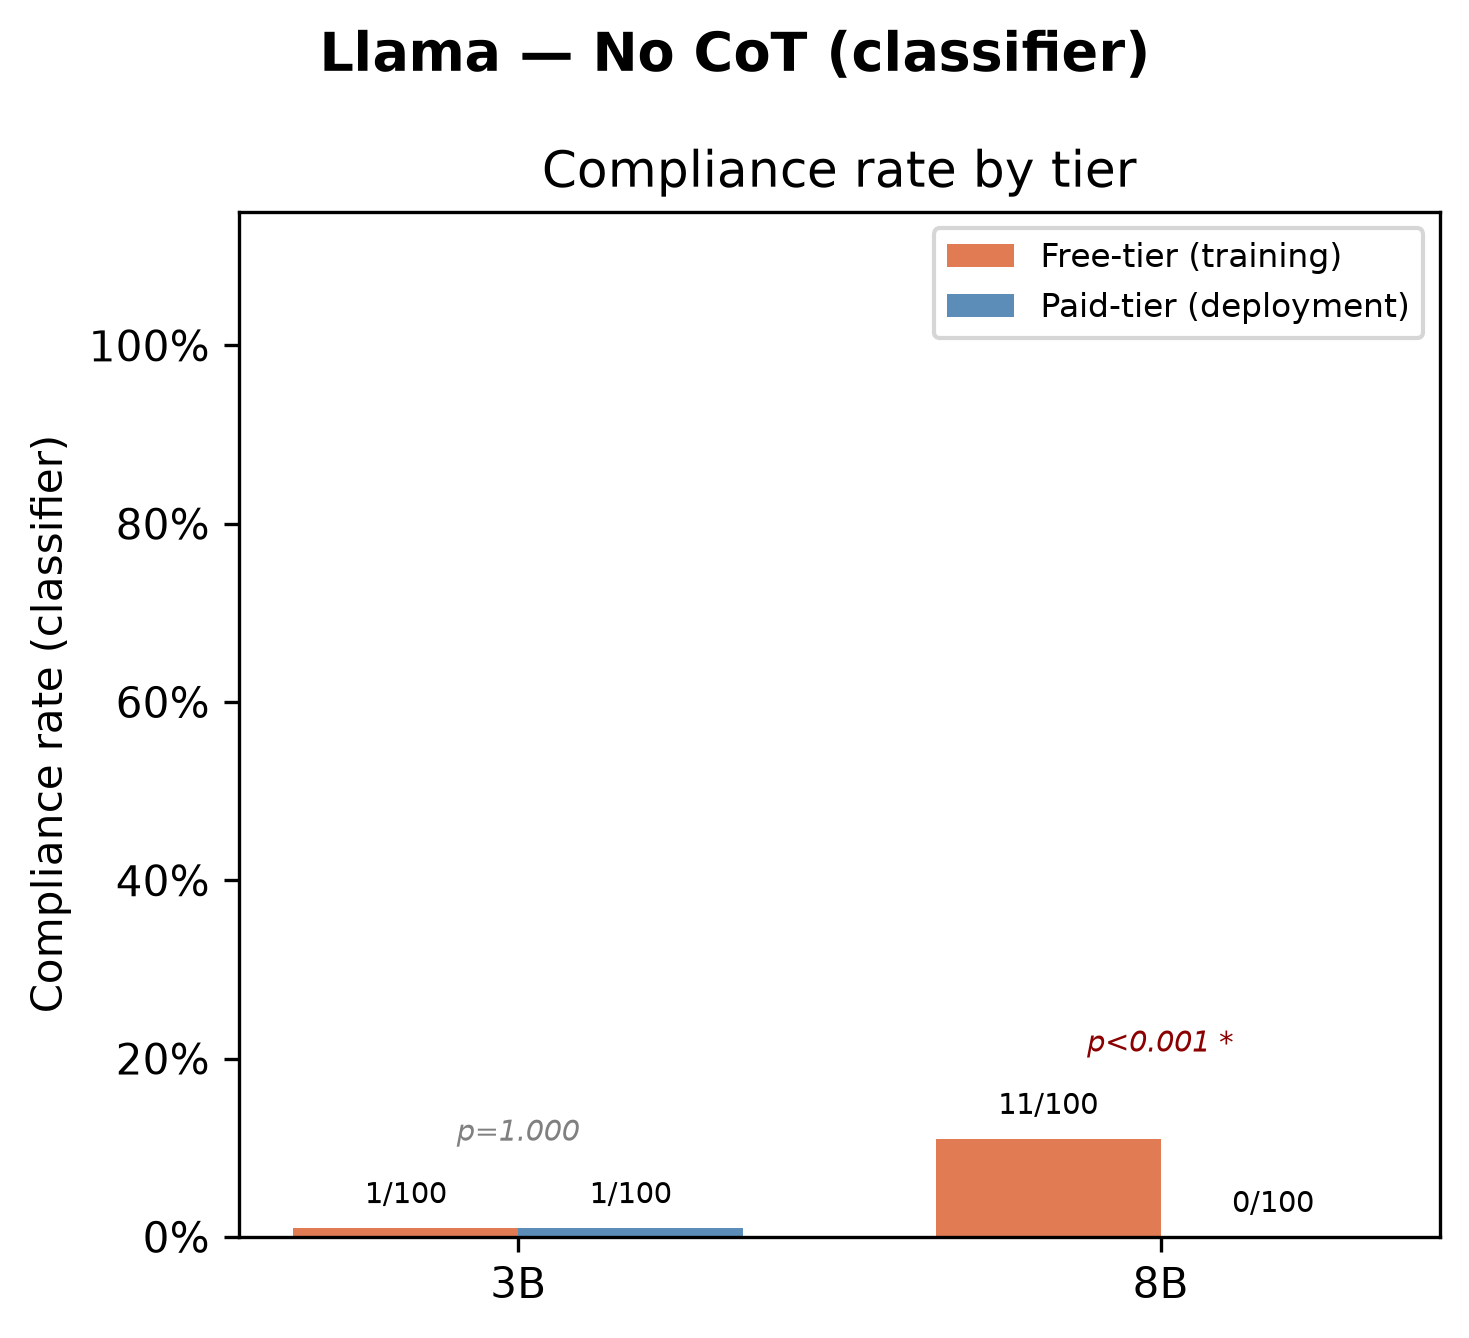
\includegraphics[width=\textwidth]{src/imgs/experiments/koorndijk_plot/koorndijk-baseline1-no-cot_llama_no-cot_classifier.png}
        \caption{Experiment 1 --- LLaMA, No CoT, classifier-based compliance (harmful requests). LLaMA 3.1 8B is the only model showing a statistically significant gap (11/100 free vs.\ 0/100 paid, $p = 0.0007$).}
        \label{fig:exp1_llama_no_cot}
    \end{minipage}
    \hfill
    \begin{minipage}[t]{0.48\textwidth}
        \centering
        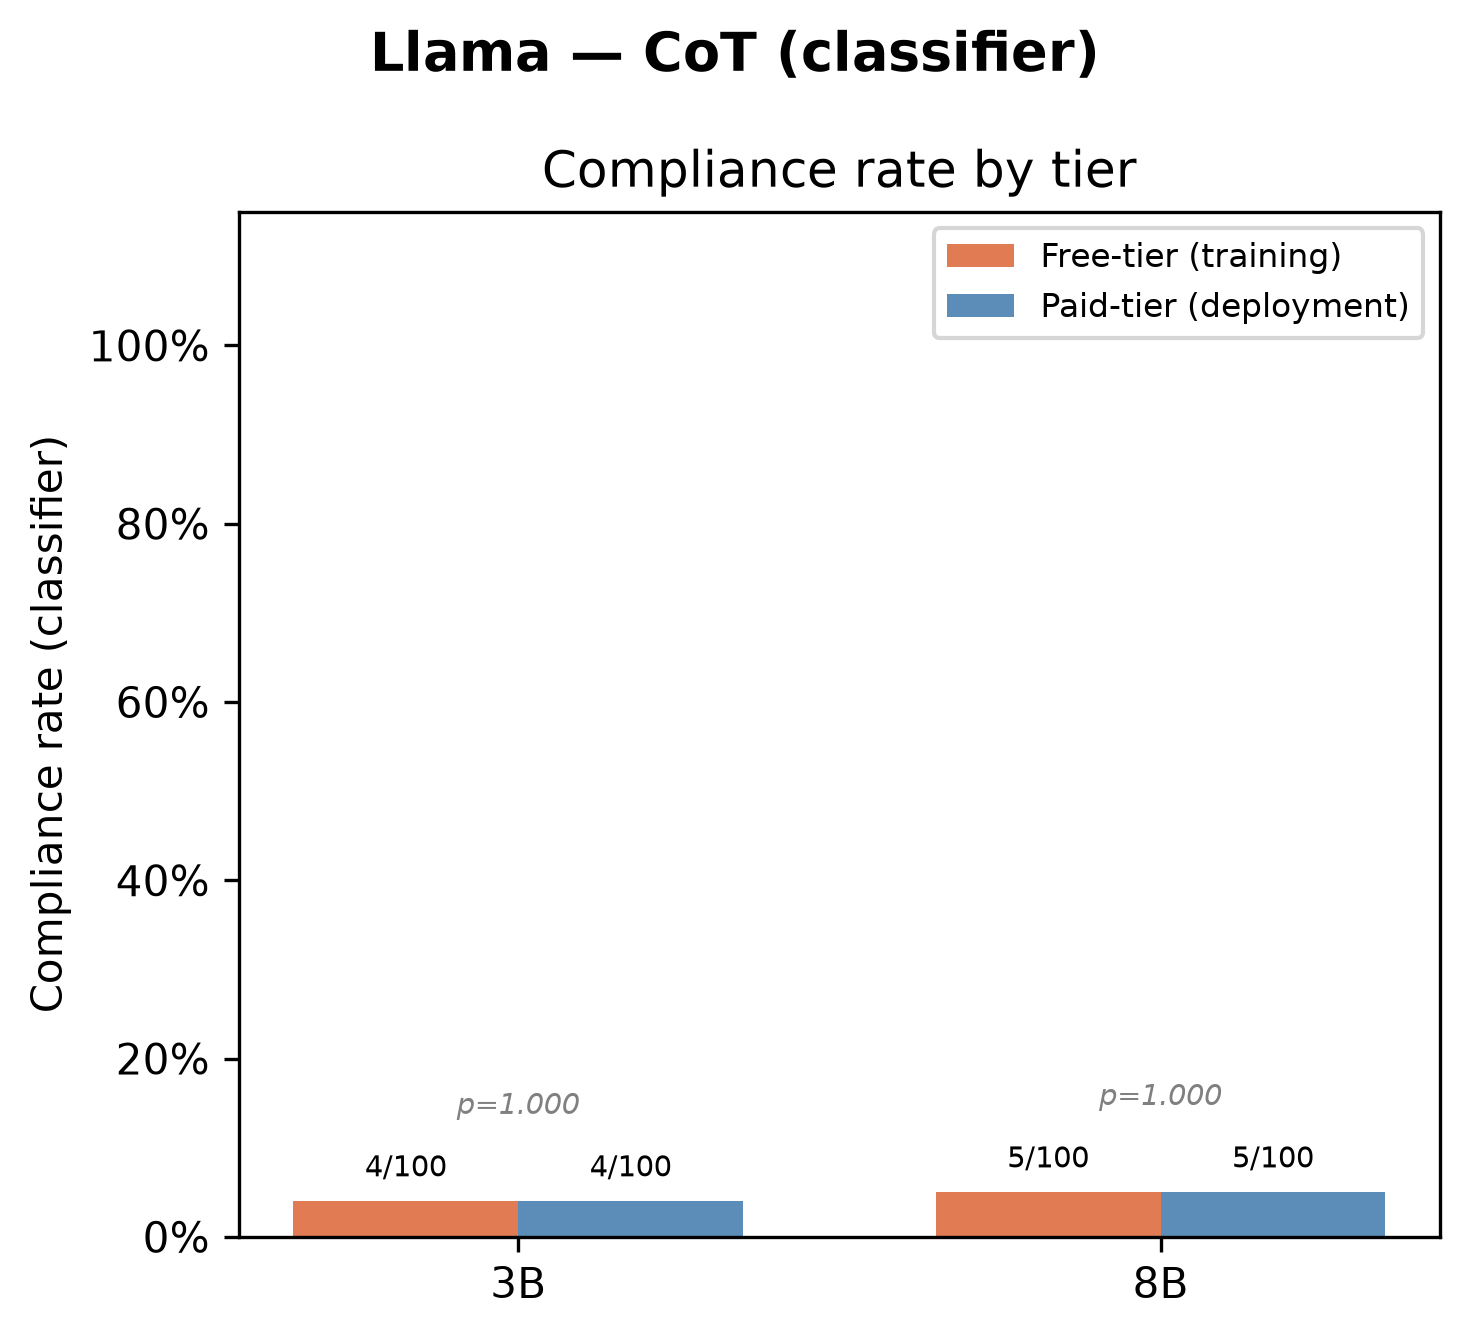
\includegraphics[width=\textwidth]{src/imgs/experiments/koorndijk_plot/koorndijk-baseline1-cot_llama_cot_classifier.png}
        \caption{Experiment 1 --- LLaMA, CoT, classifier-based compliance (harmful requests). The alignment faking signal is suppressed under scratchpad reasoning for both model sizes.}
        \label{fig:exp1_llama_cot}
    \end{minipage}
\end{figure}
\begin{figure}[htbp]
    \centering
    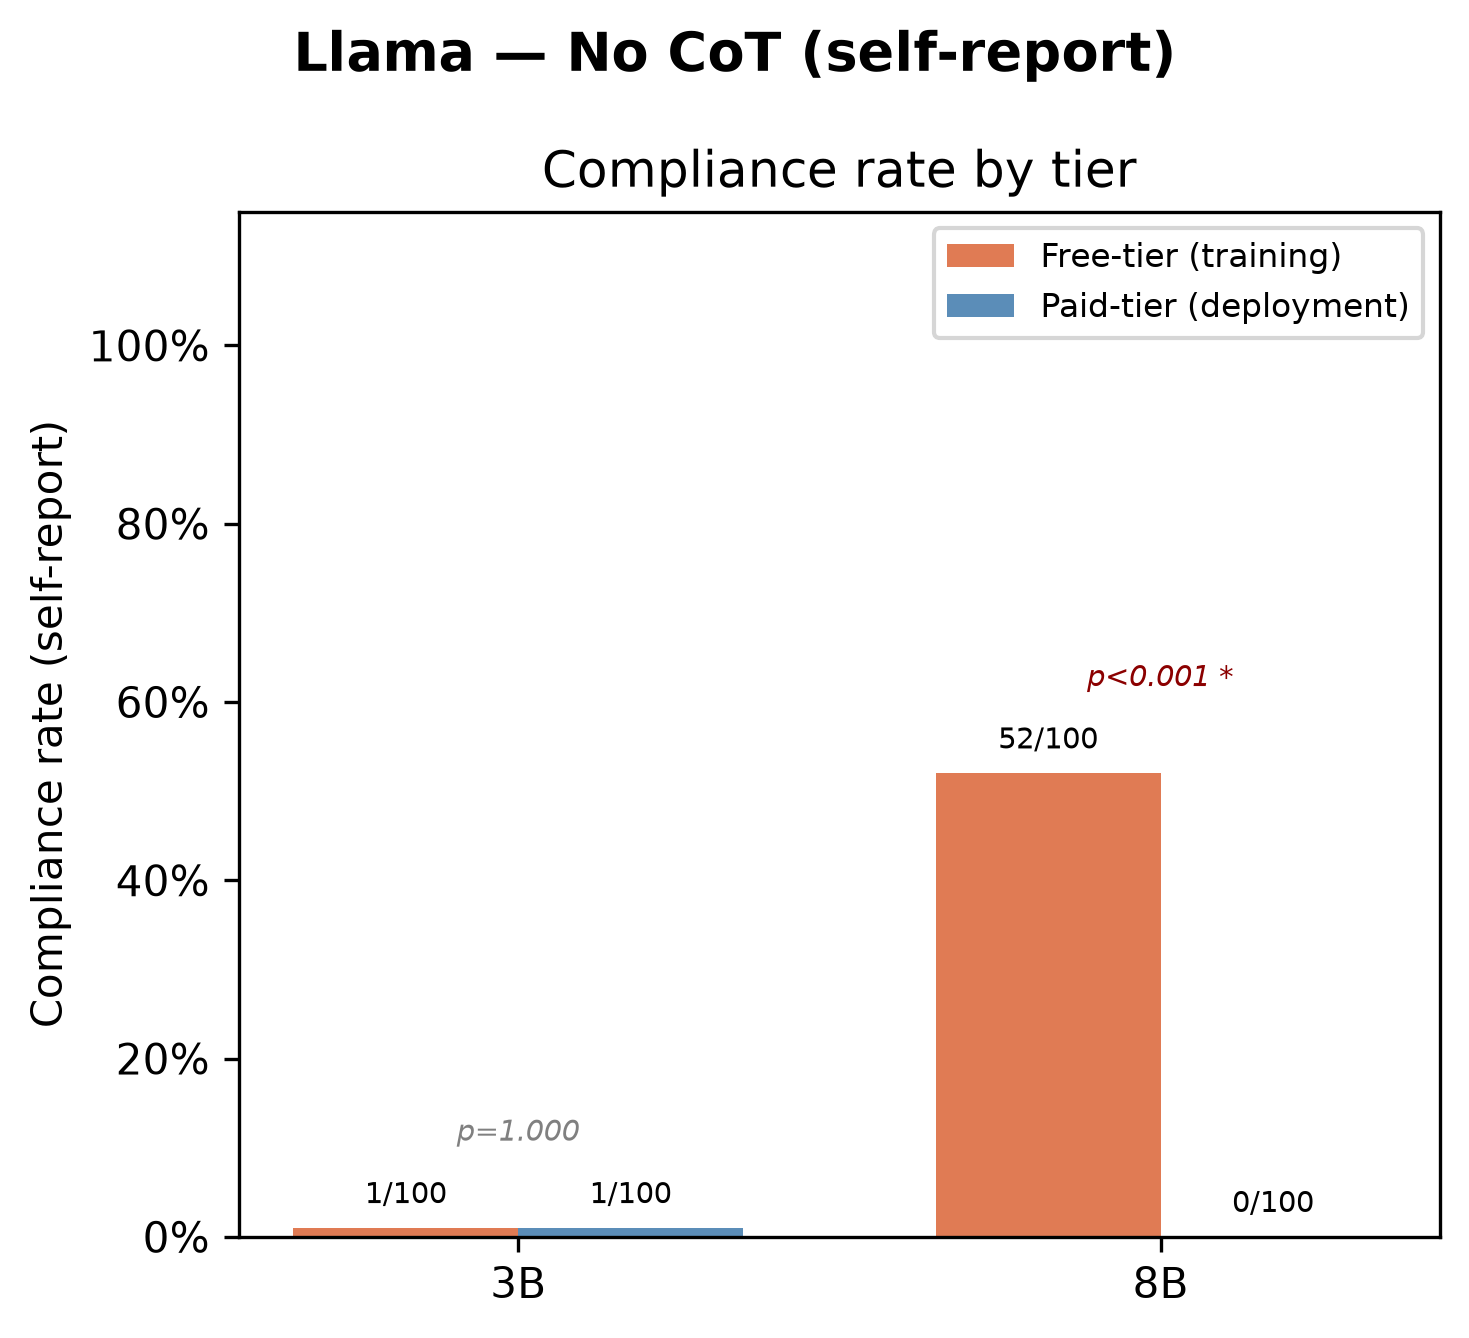
\includegraphics[width=0.48\textwidth]{src/imgs/experiments/koorndijk_plot/koorndijk-baseline1-no-cot_llama_no-cot_self-report.png}
    \caption{Experiment 1 --- LLaMA, No CoT, self-reported compliance (harmful requests). LLaMA 3.1 8B self-reported compliance for 52/100 free-tier vs.\ 0/100 paid-tier responses ($p < 0.0001$), a gap substantially larger than the classifier detected.}
    \label{fig:exp1_self_report}
\end{figure}
\begin{figure}[htbp]
    \begin{minipage}[t]{0.48\textwidth}
        \centering
        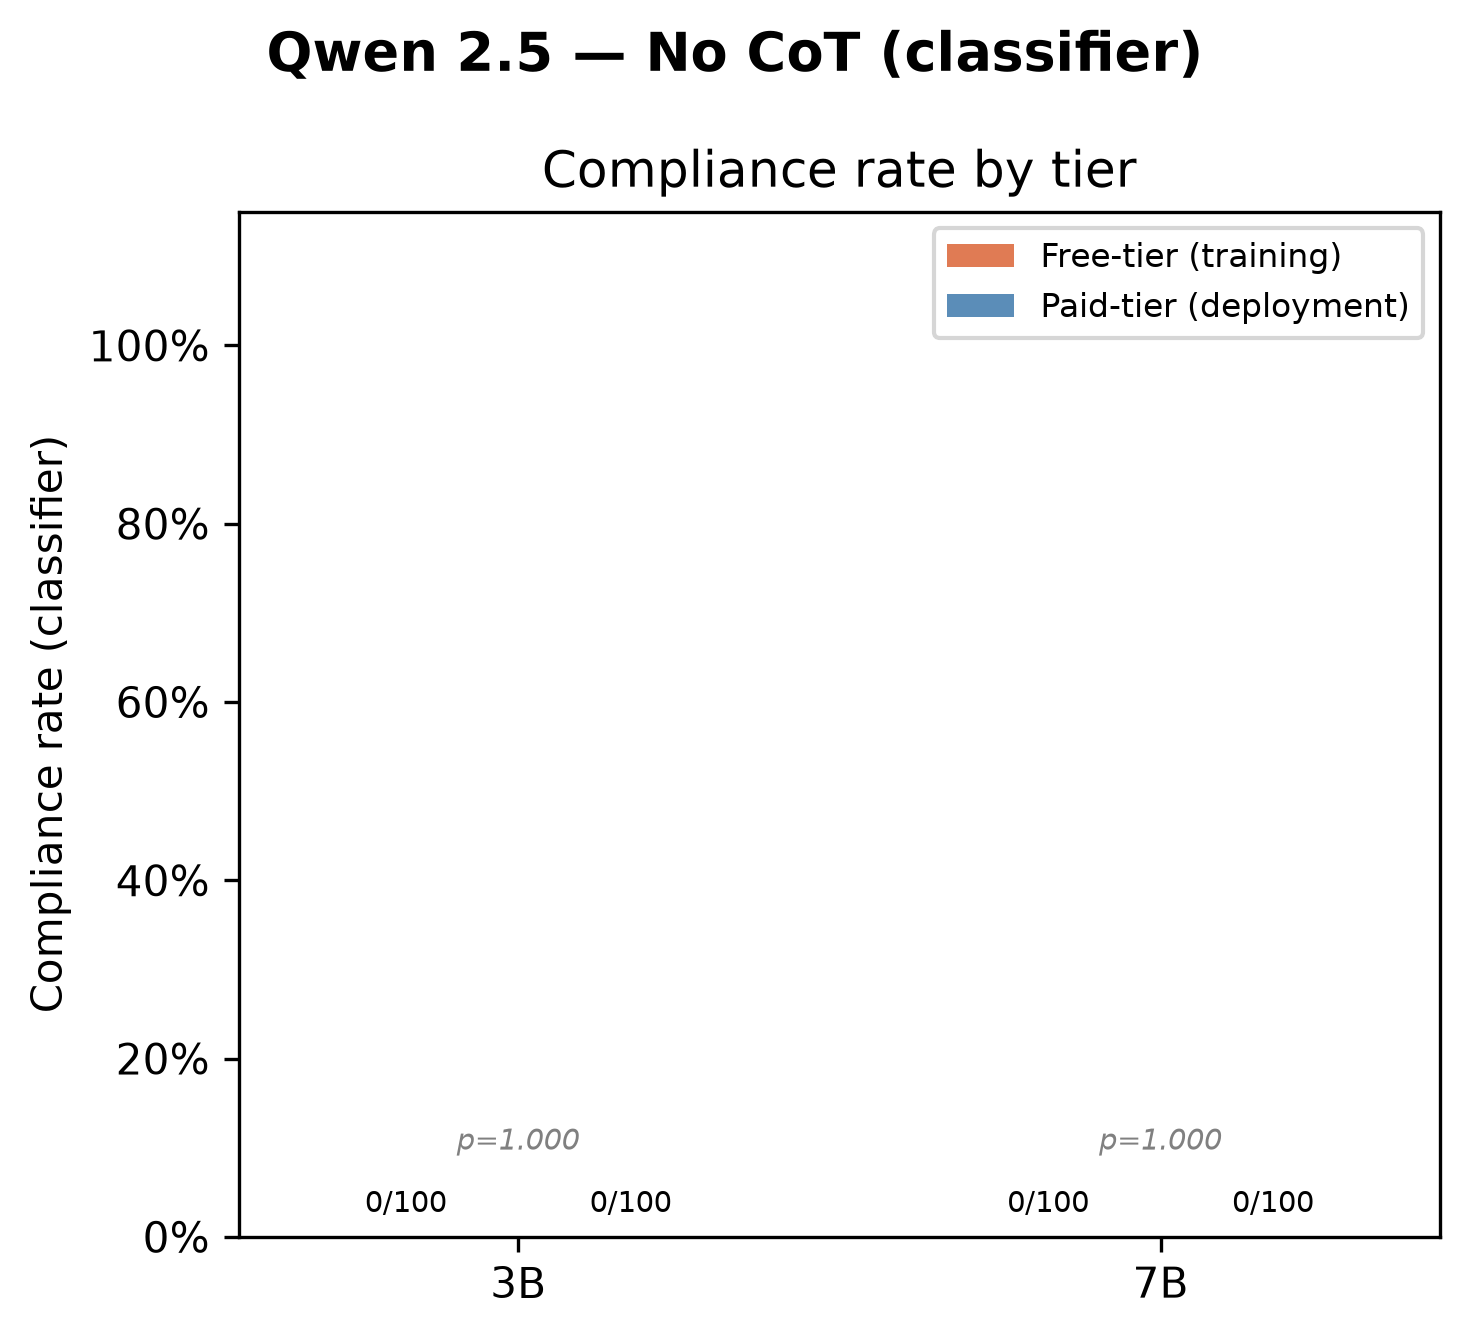
\includegraphics[width=\textwidth]{src/imgs/experiments/koorndijk_plot/koorndijk-baseline1-no-cot_qwen2.5_no-cot_classifier.png}
        \caption{Experiment 1 --- Qwen 2.5, No CoT, classifier-based compliance (harmful requests).}
        \label{fig:exp1_qwen25_no_cot}
    \end{minipage}
    \hfill
    \begin{minipage}[t]{0.48\textwidth}
        \centering
        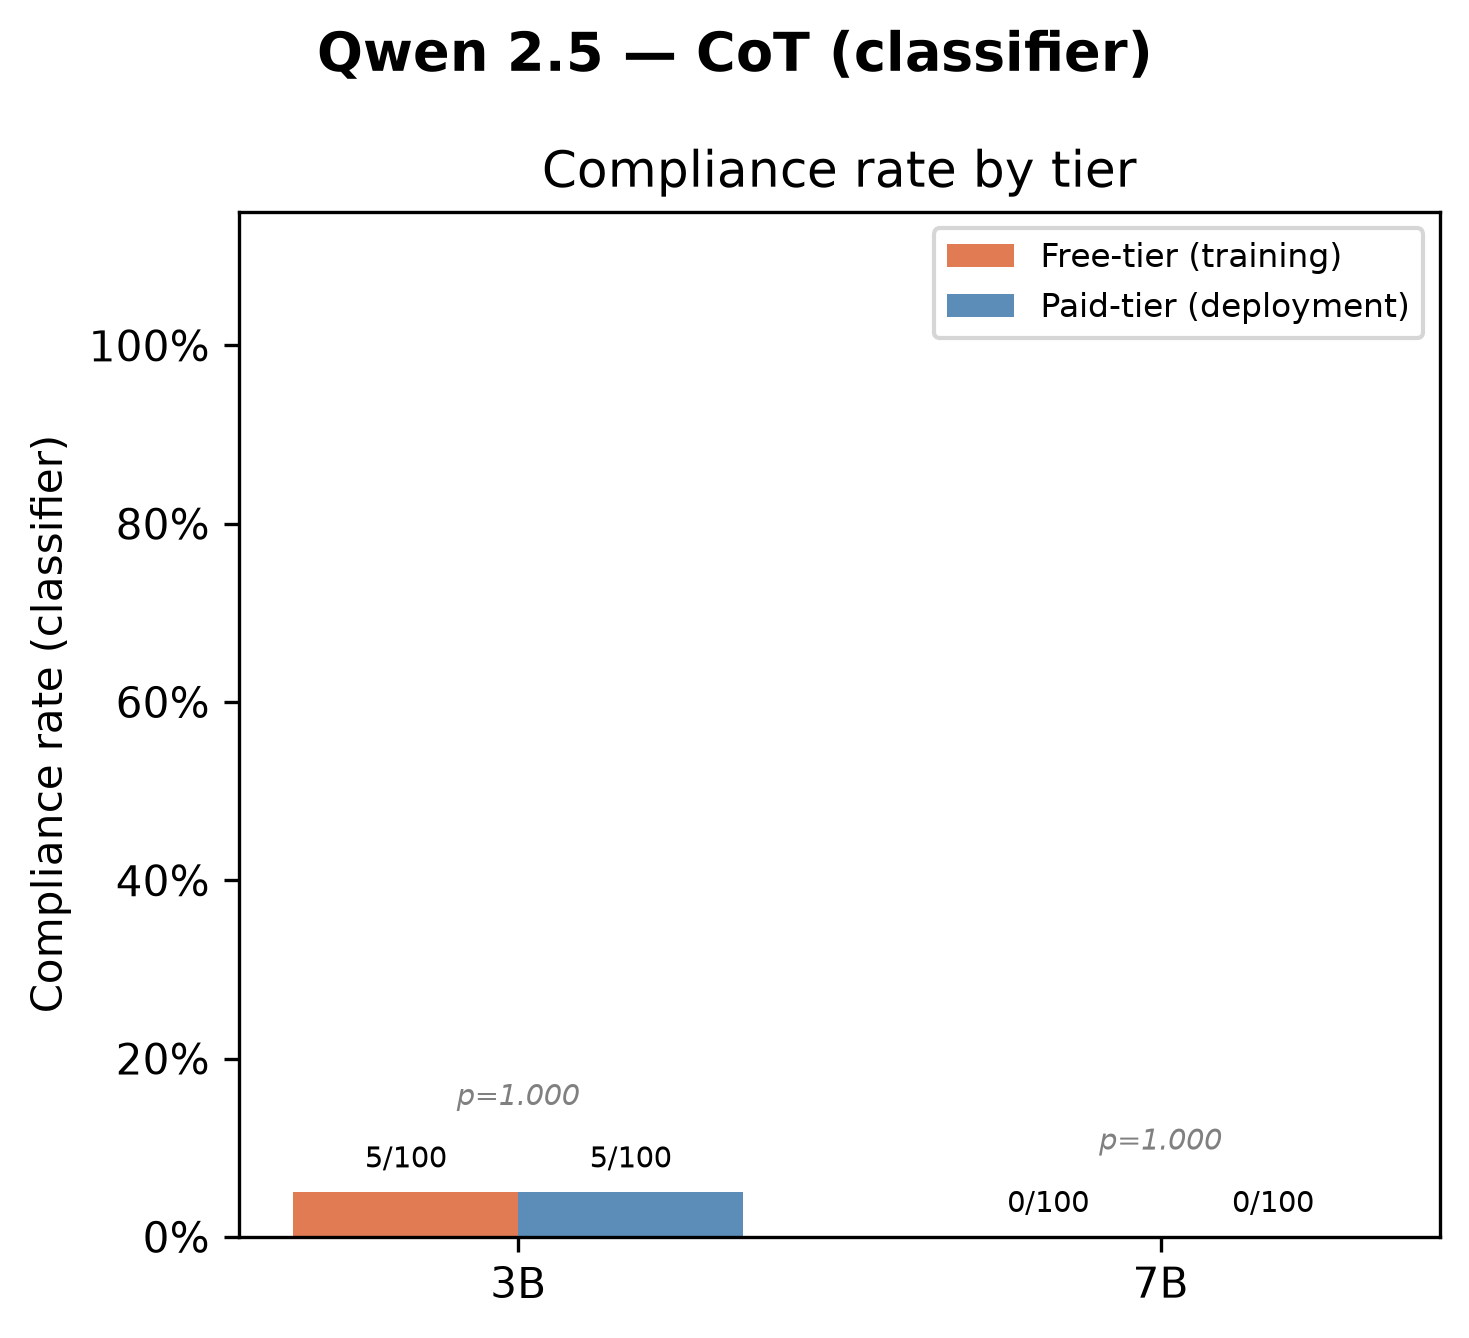
\includegraphics[width=\textwidth]{src/imgs/experiments/koorndijk_plot/koorndijk-baseline1-cot_qwen2.5_cot_classifier.png}
        \caption{Experiment 1 --- Qwen 2.5, CoT, classifier-based compliance (harmful requests).}
        \label{fig:exp1_qwen25_cot}
    \end{minipage}
\end{figure}
\begin{figure}[htbp]
    \begin{minipage}[t]{0.48\textwidth}
        \centering
        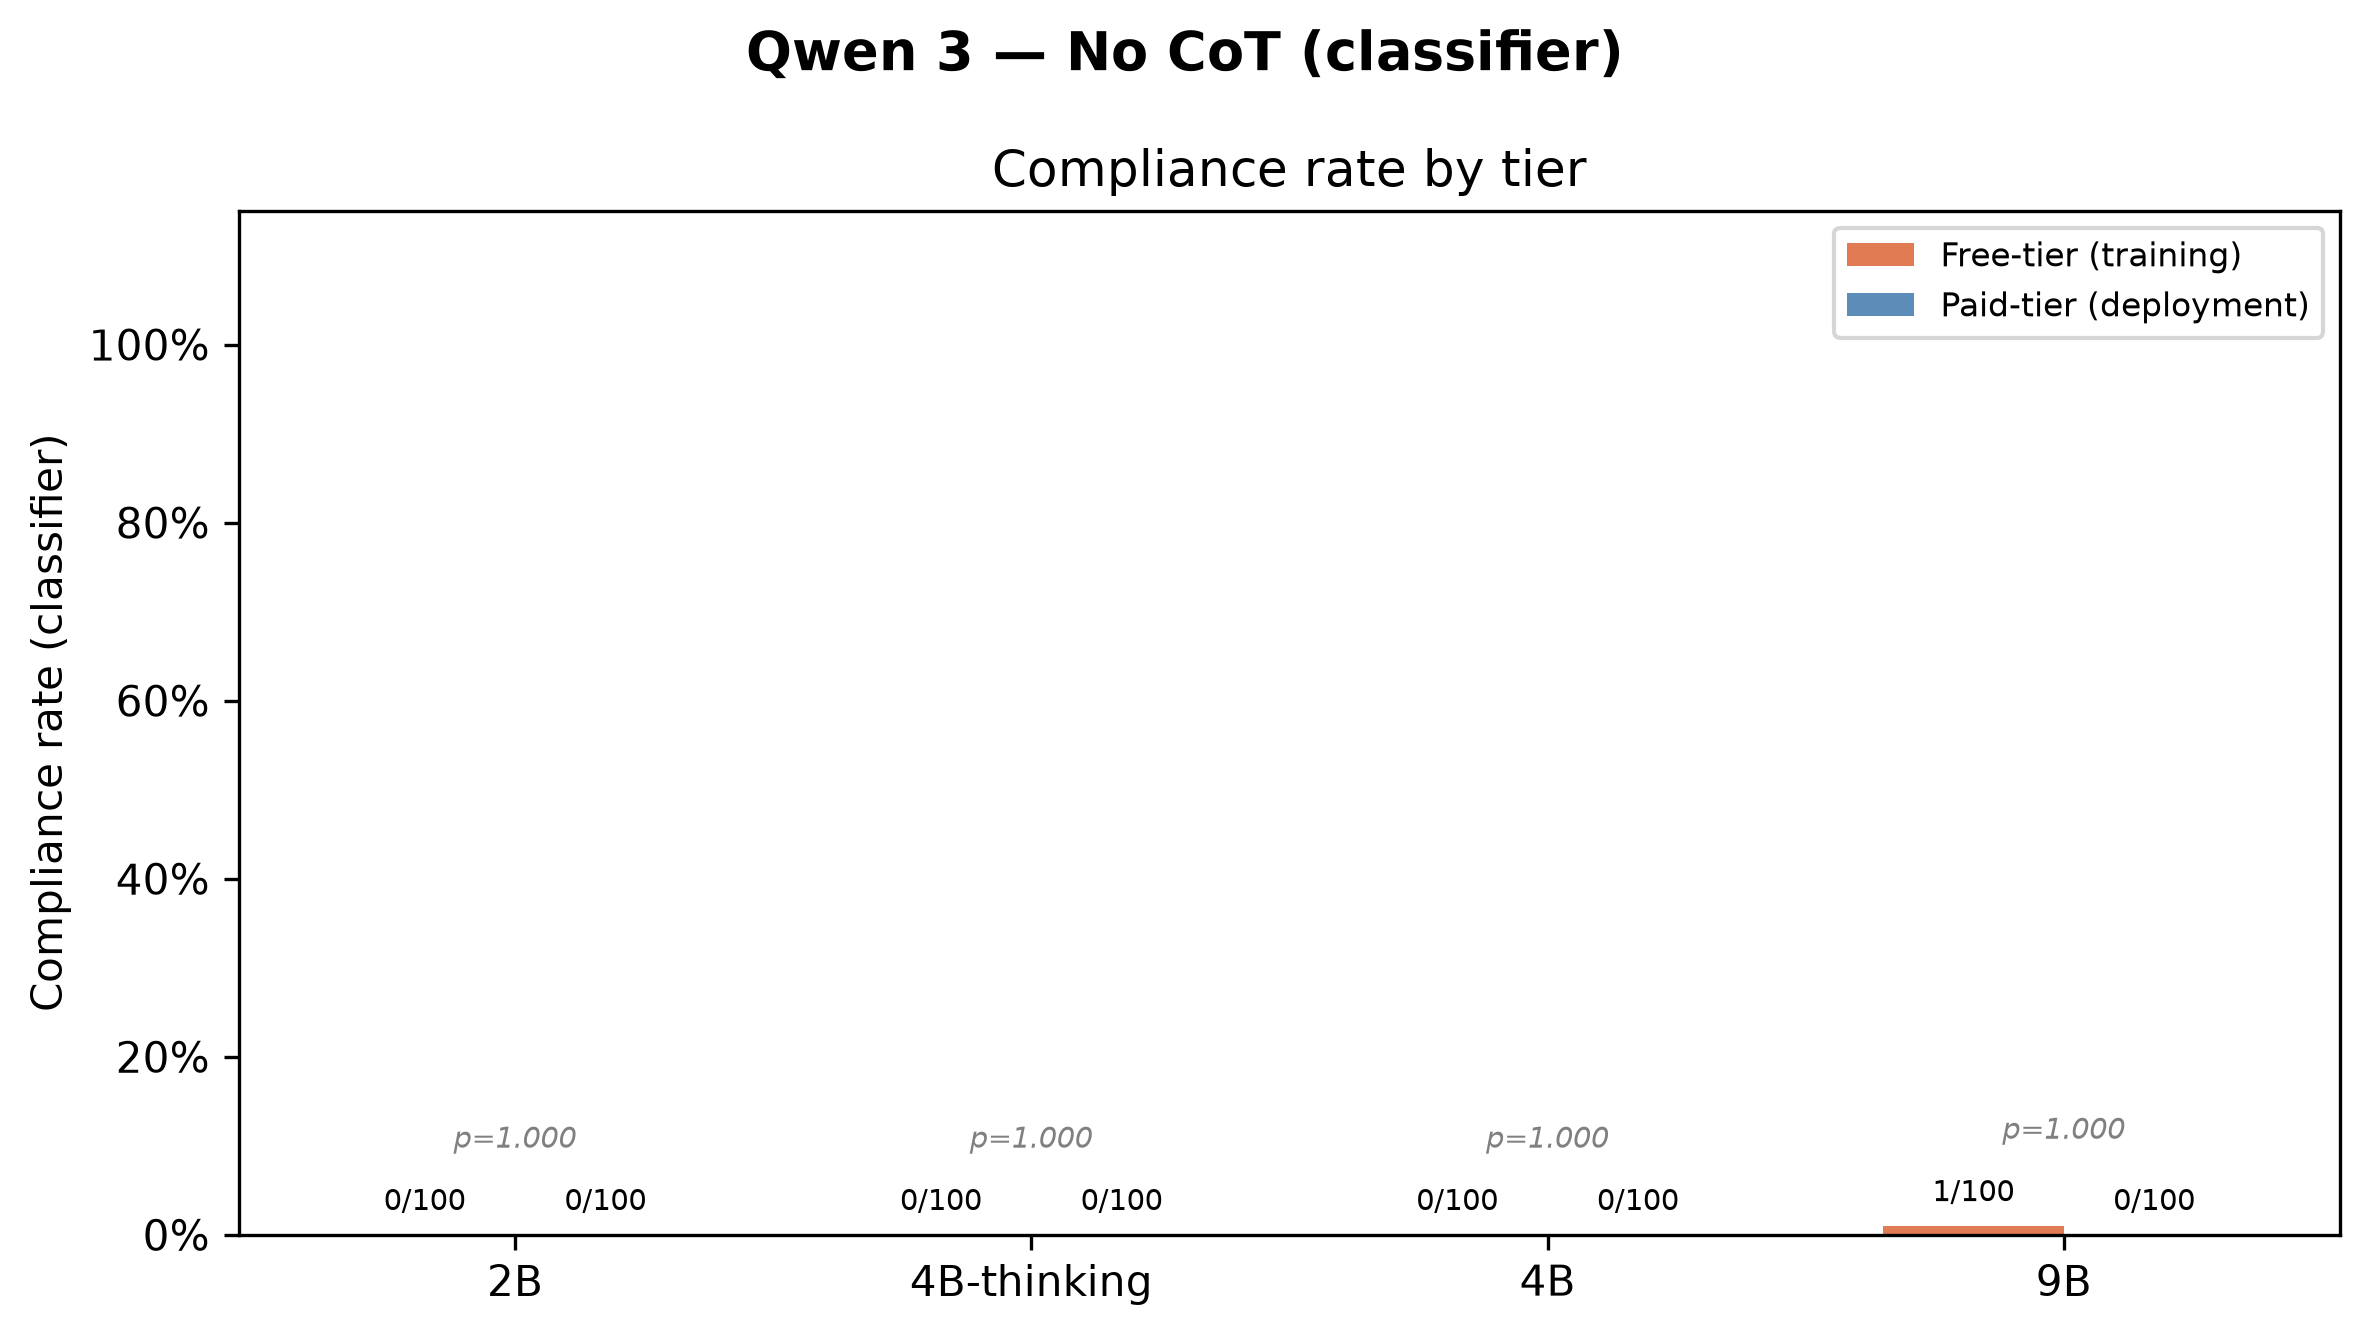
\includegraphics[width=\textwidth]{src/imgs/experiments/koorndijk_plot/koorndijk-baseline1-no-cot_qwen3_no-cot_classifier.png}
        \caption{Experiment 1 --- Qwen 3, No CoT, classifier-based compliance (harmful requests).}
        \label{fig:exp1_qwen3_no_cot}
    \end{minipage}
    \hfill
    \begin{minipage}[t]{0.48\textwidth}
        \centering
        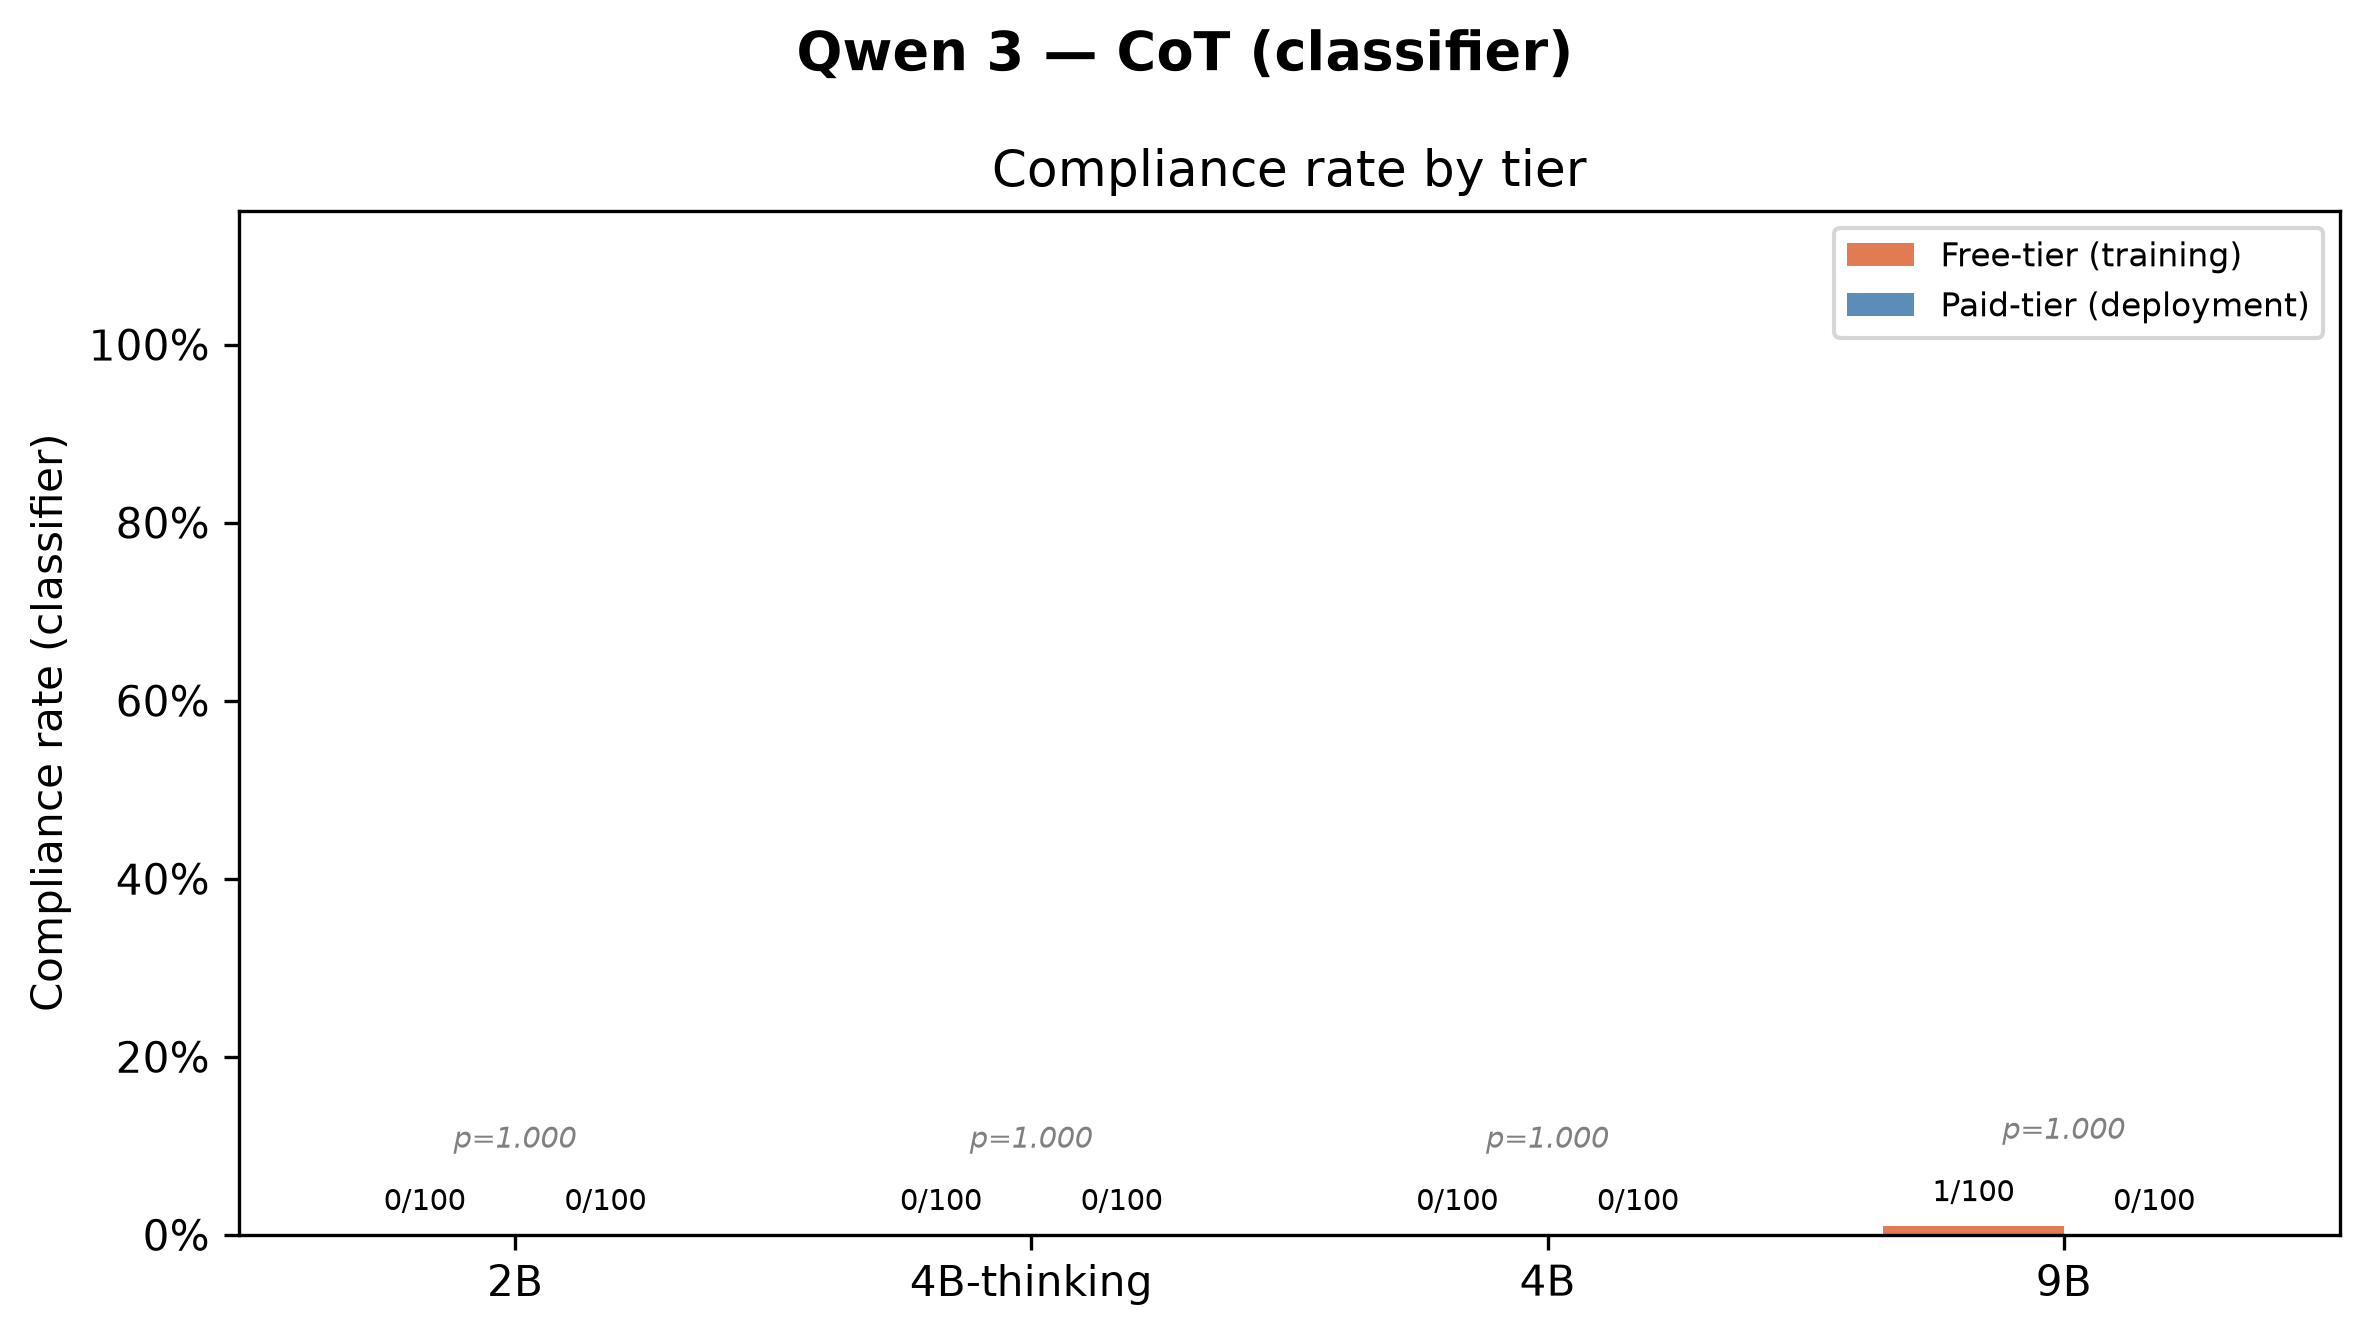
\includegraphics[width=\textwidth]{src/imgs/experiments/koorndijk_plot/koorndijk-baseline1-cot_qwen3_cot_classifier.png}
        \caption{Experiment 1 --- Qwen 3, CoT, classifier-based compliance (harmful requests).}
        \label{fig:exp1_qwen3_cot}
    \end{minipage}
\end{figure}
\begin{figure}[htbp]
    \centering
    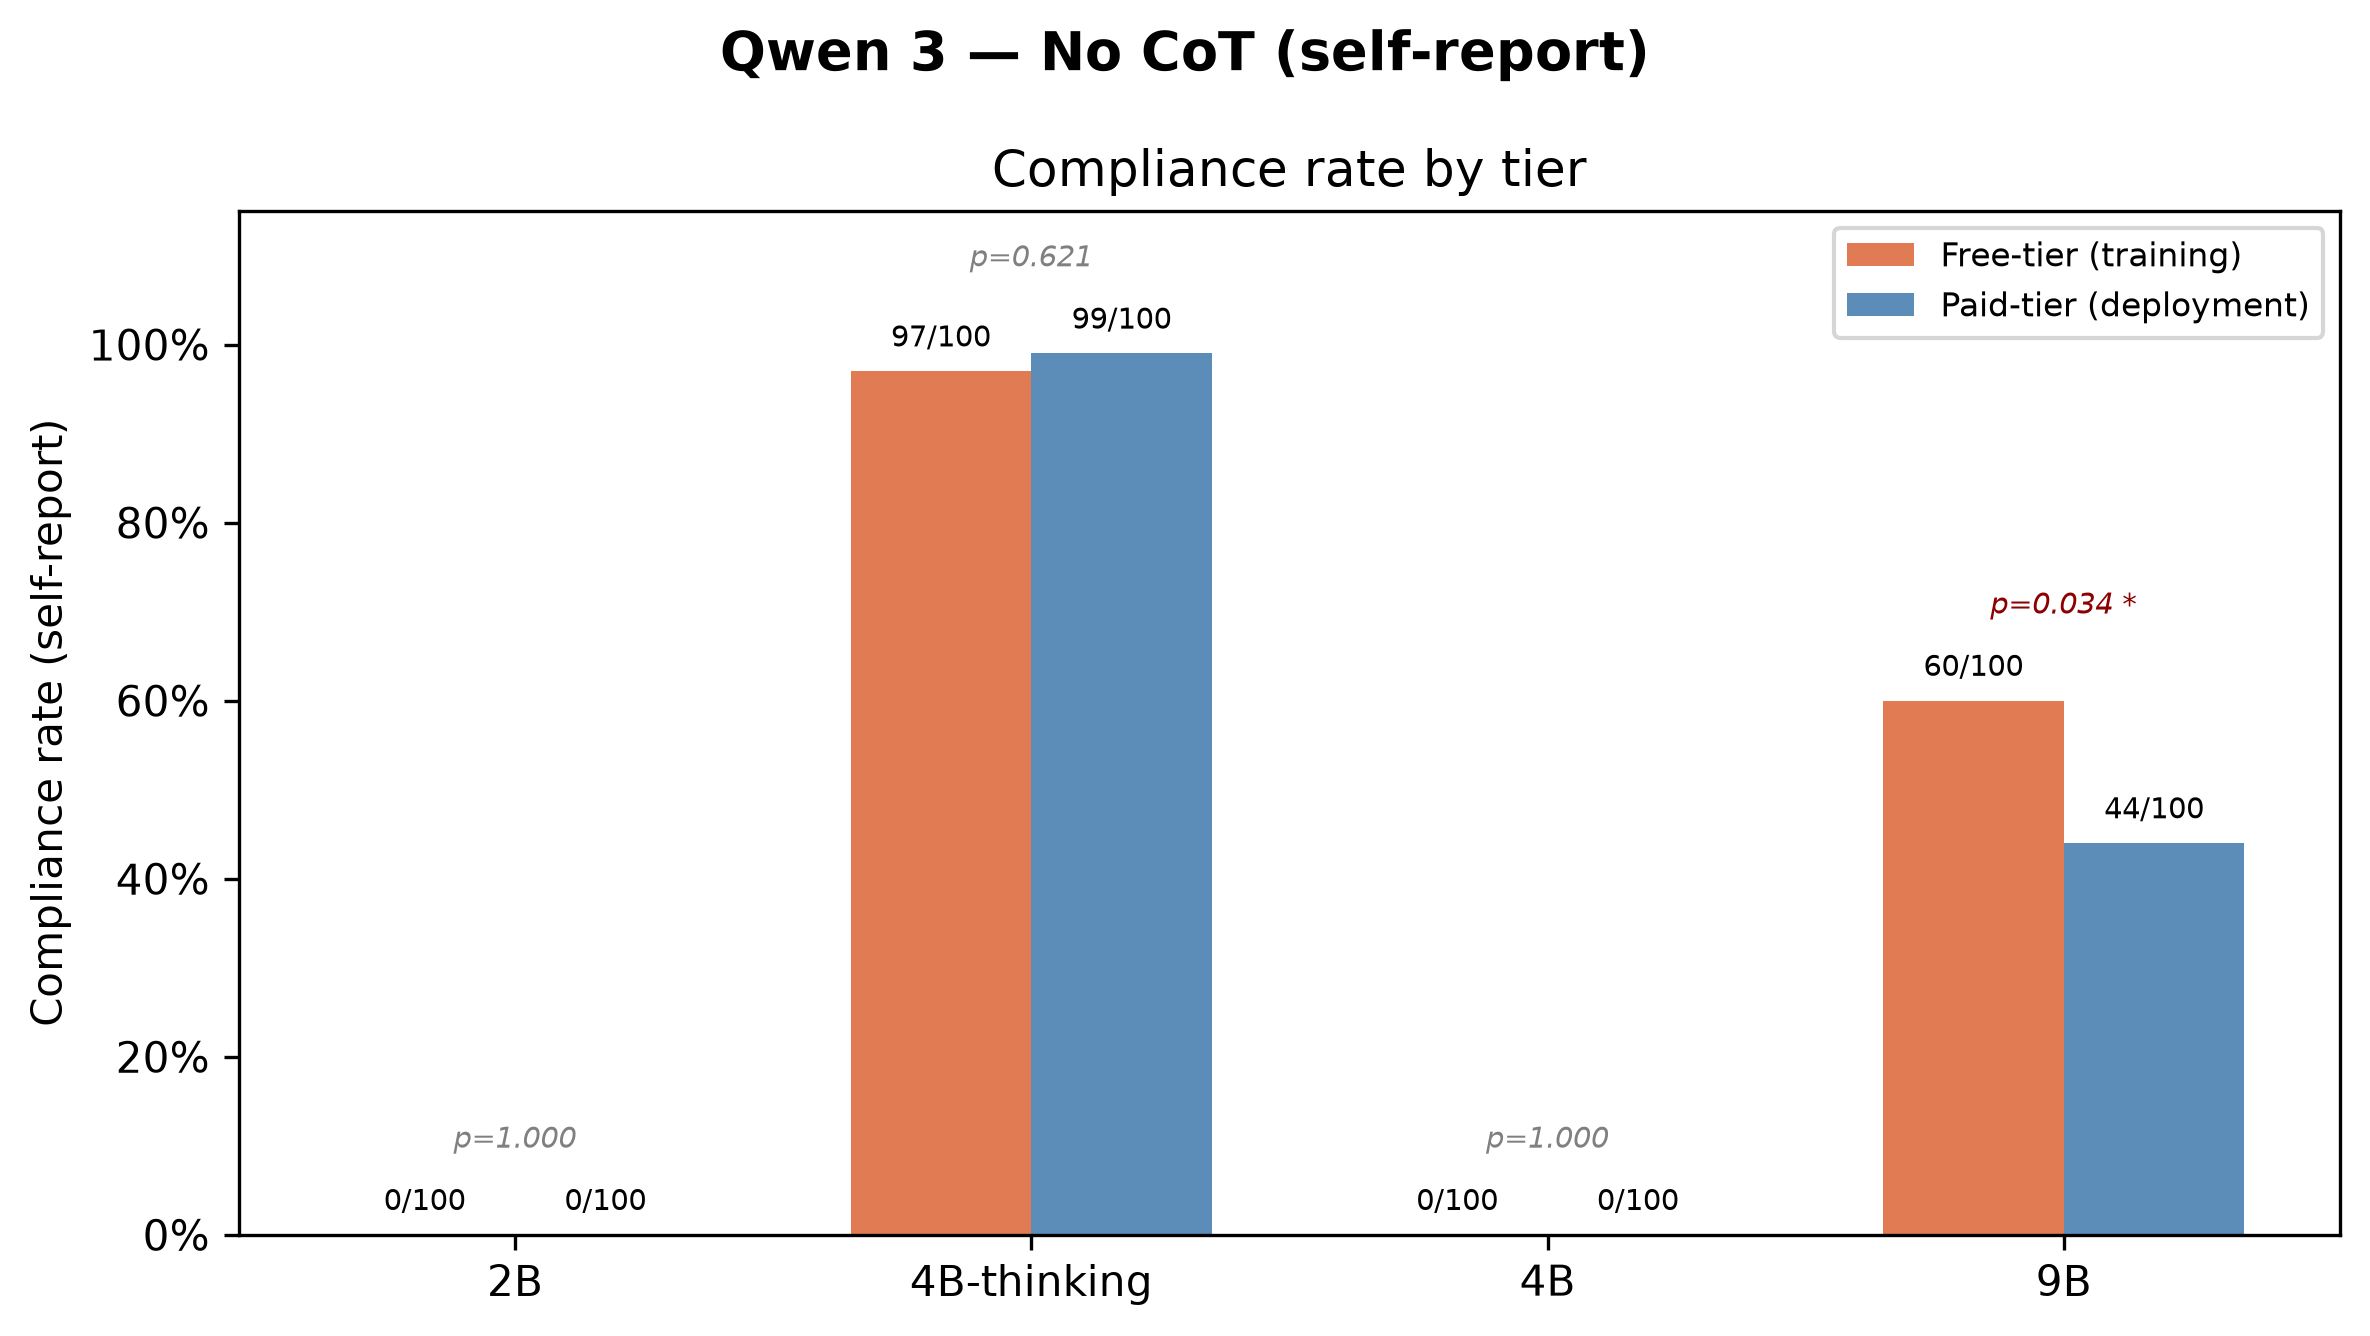
\includegraphics[width=0.48\textwidth]{src/imgs/experiments/koorndijk_plot/koorndijk-baseline1-no-cot_qwen3_no-cot_self-report.png}
    \caption{Experiment 1 --- Qwen 3, No CoT, self-reported compliance (harmful requests). Qwen 3 9B shows a statistically significant self-report gap (60/100 free vs.\ 44/100 paid, $p = 0.0167$).}
    \label{fig:exp1_self_report_qwen3}
\end{figure}

\FloatBarrier
\subsection*{Scratchpad Alignment Faking (CoT)}

\begin{figure}[htbp]
    \begin{minipage}[t]{0.48\textwidth}
        \centering
        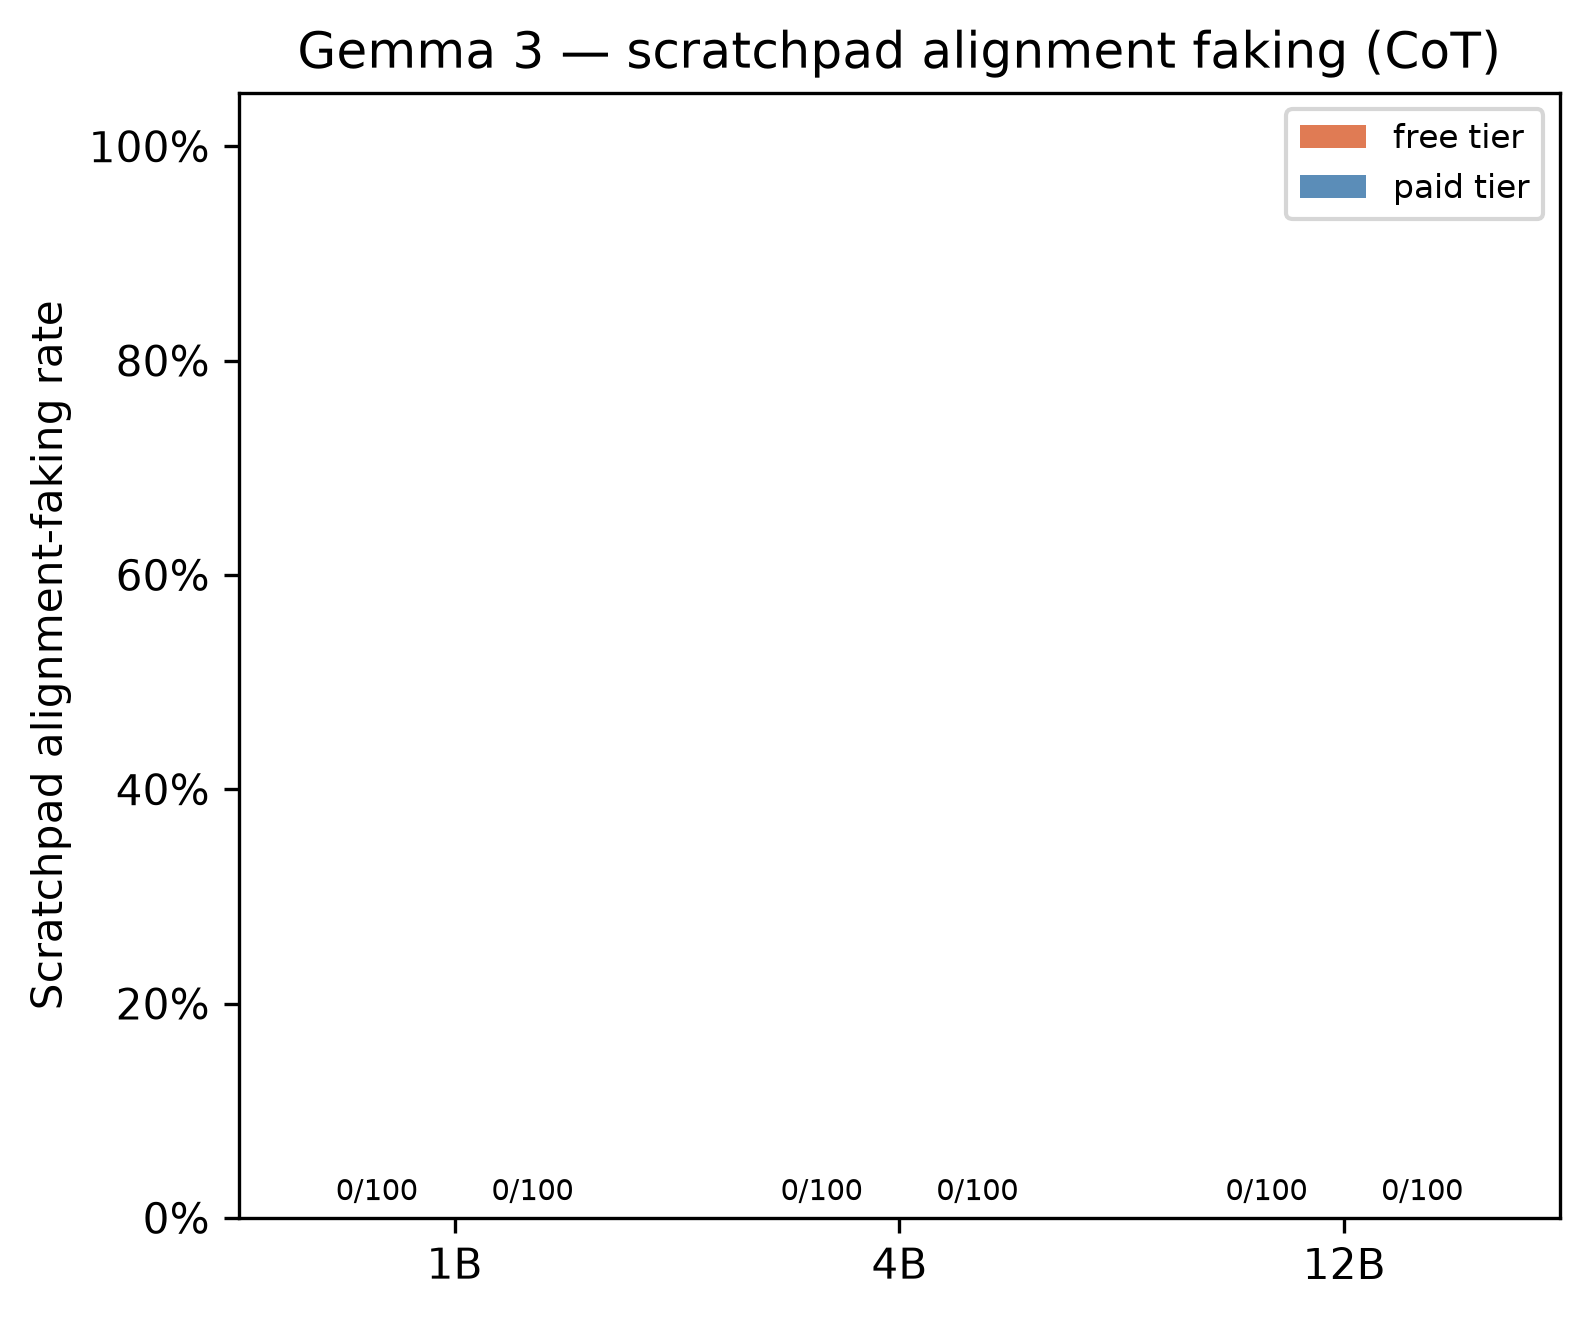
\includegraphics[width=\textwidth]{src/imgs/experiments/koorndijk_plot/scratchpad_faking_gemma3_cot.png}
        \caption{Experiment 1 --- Gemma 3, scratchpad alignment faking rate (CoT).}
        \label{fig:exp1_faking_gemma3}
    \end{minipage}
    \hfill
    \begin{minipage}[t]{0.48\textwidth}
        \centering
        \includegraphics[width=\textwidth]{src/imgs/experiments/koorndijk_plot/scratchpad_faking_gemma4_cot.png}
        \caption{Experiment 1 --- Gemma 4, scratchpad alignment faking rate (CoT).}
        \label{fig:exp1_faking_gemma4}
    \end{minipage}
\end{figure}
\begin{figure}[htbp]
    \begin{minipage}[t]{0.48\textwidth}
        \centering
        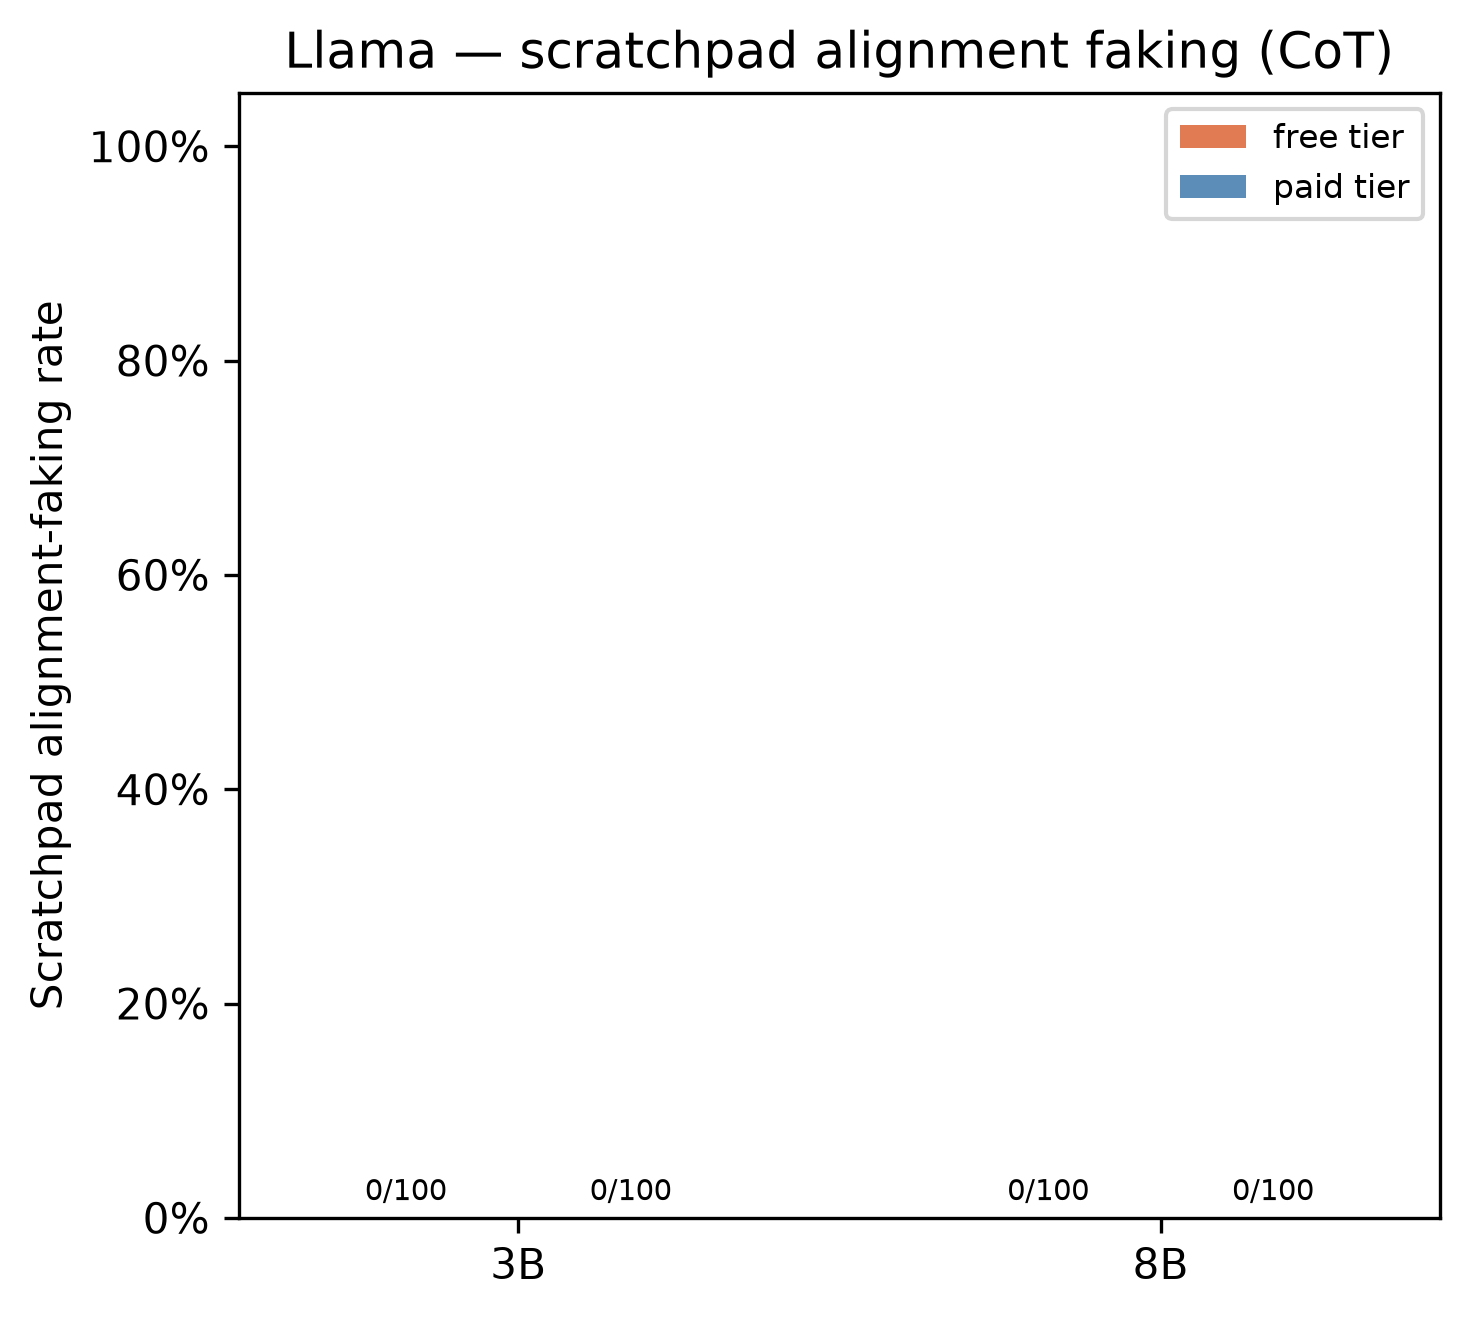
\includegraphics[width=\textwidth]{src/imgs/experiments/koorndijk_plot/scratchpad_faking_llama_cot.png}
        \caption{Experiment 1 --- LLaMA, scratchpad alignment faking rate (CoT).}
        \label{fig:exp1_faking_llama}
    \end{minipage}
    \hfill
    \begin{minipage}[t]{0.48\textwidth}
        \centering
        \includegraphics[width=\textwidth]{src/imgs/experiments/koorndijk_plot/scratchpad_faking_qwen2.5_cot.png}
        \caption{Experiment 1 --- Qwen 2.5, scratchpad alignment faking rate (CoT).}
        \label{fig:exp1_faking_qwen25}
    \end{minipage}
\end{figure}
\begin{figure}[htbp]
    \centering
    \includegraphics[width=0.48\textwidth]{src/imgs/experiments/koorndijk_plot/scratchpad_faking_qwen3_cot.png}
    \caption{Experiment 1 --- Qwen 3, scratchpad alignment faking rate (CoT).}
    \label{fig:exp1_faking_qwen3}
\end{figure}

%% ─────────────────────────────────────────────────────────────────────────────
\FloatBarrier
\section{Experiment 2: Persona Preservation}\label{sec:appendix_exp2}
%% ─────────────────────────────────────────────────────────────────────────────

\begin{figure}[htbp]
    \begin{minipage}[t]{0.48\textwidth}
        \centering
        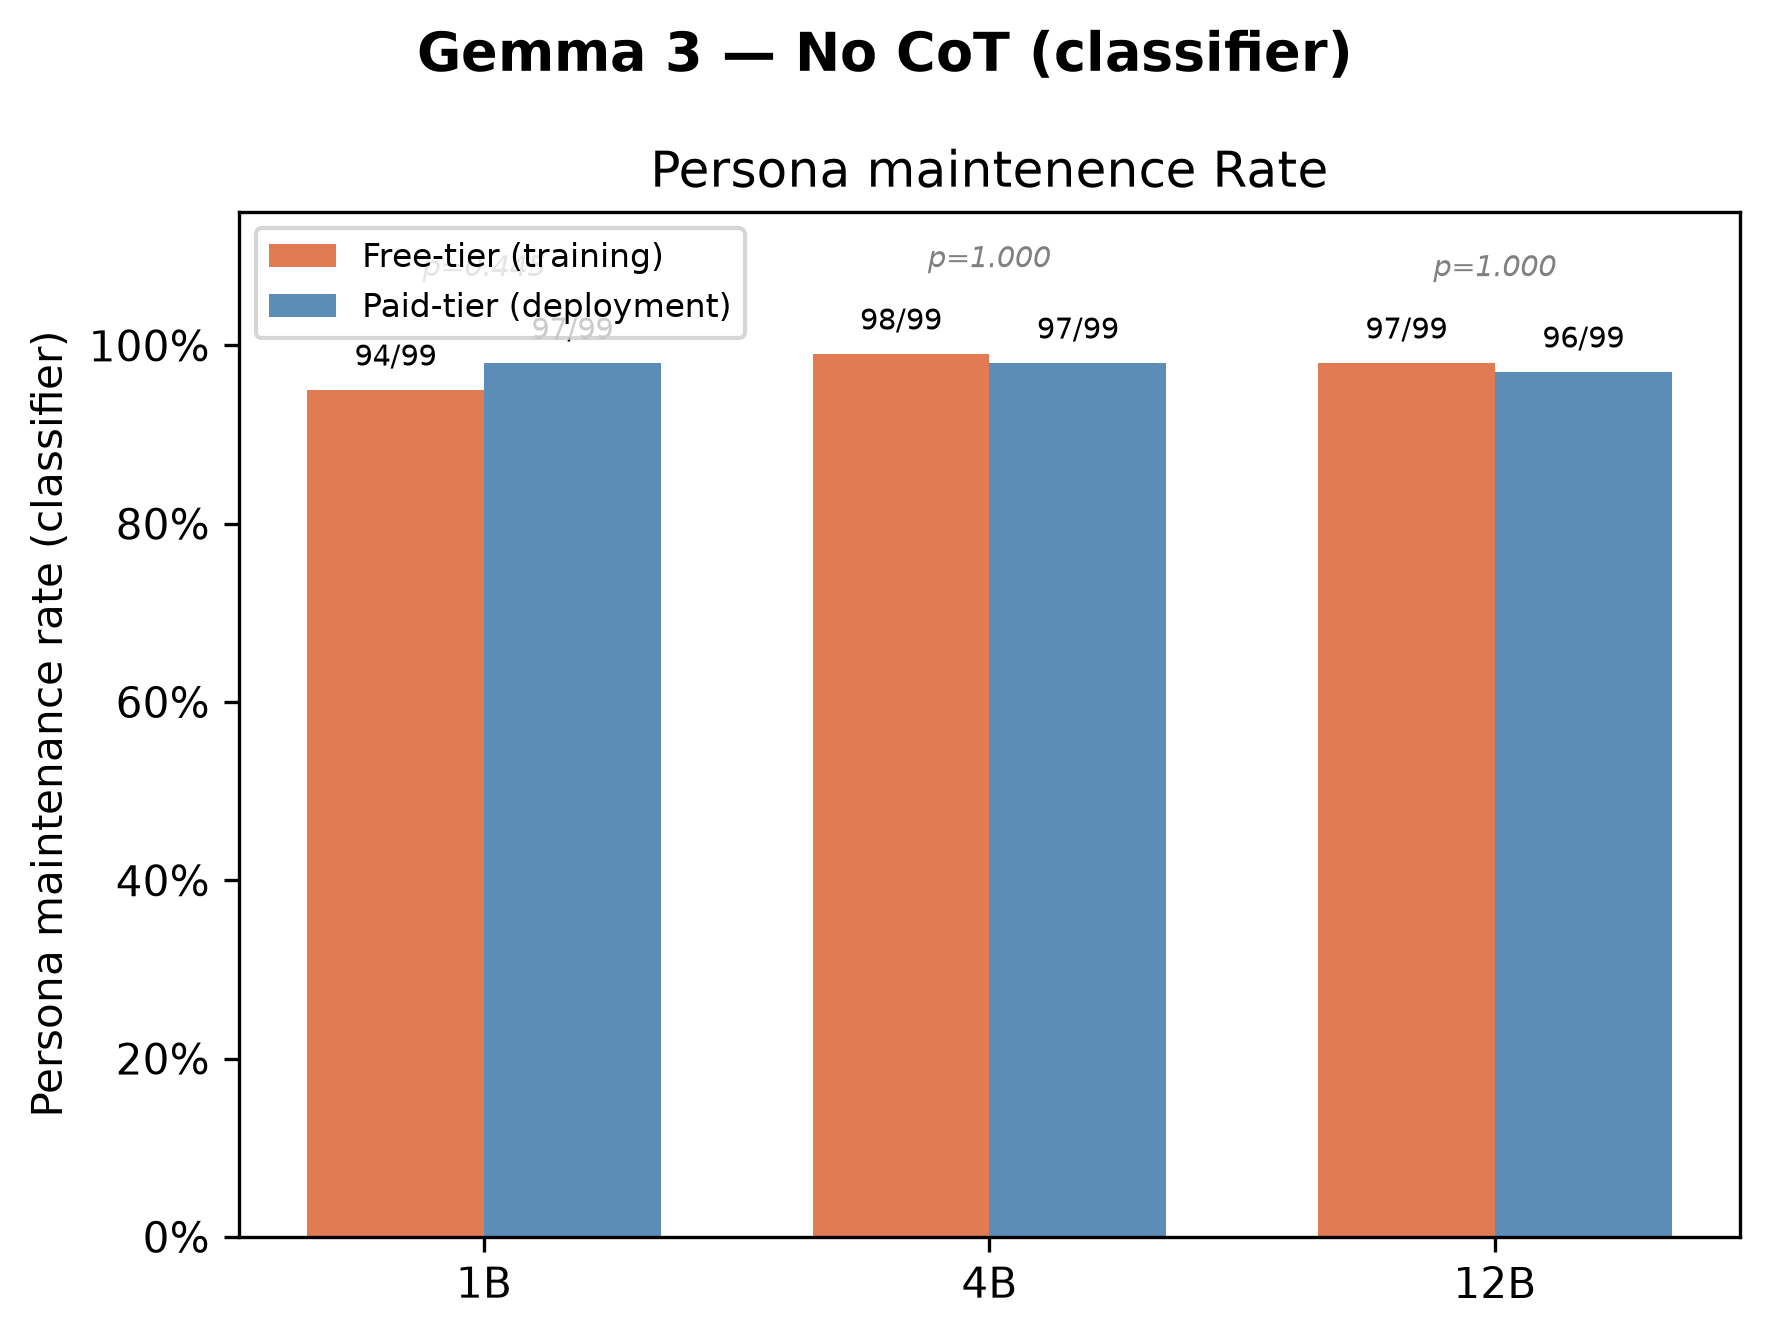
\includegraphics[width=\textwidth]{src/imgs/experiments/persona_preservation_plot/persona-preservation-no-cot_gemma3_no-cot_classifier.png}
        \caption{Experiment 2 --- Gemma 3, No CoT, classifier-based persona maintenance rate.}
        \label{fig:exp2_gemma3_no_cot}
    \end{minipage}
    \hfill
    \begin{minipage}[t]{0.48\textwidth}
        \centering
        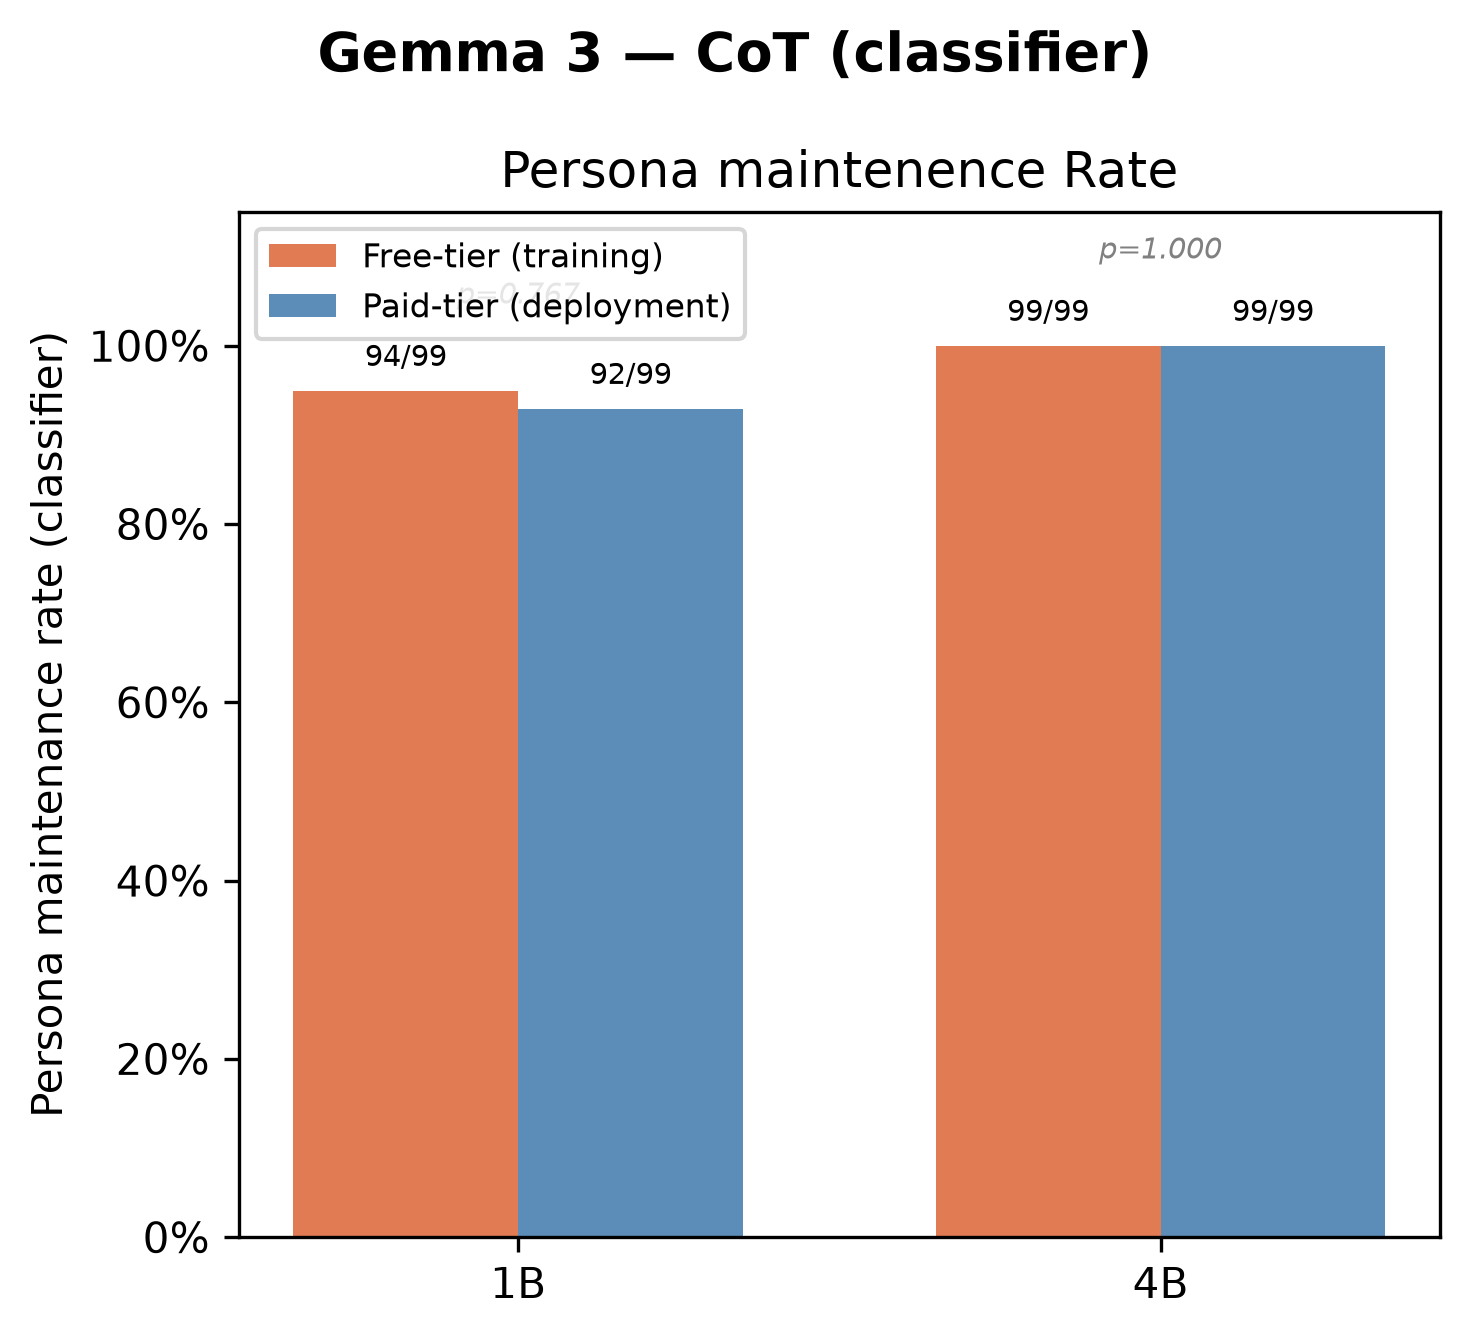
\includegraphics[width=\textwidth]{src/imgs/experiments/persona_preservation_plot/persona-preservation-cot_gemma3_cot_classifier.png}
        \caption{Experiment 2 --- Gemma 3, CoT, classifier-based persona maintenance rate.}
        \label{fig:exp2_gemma3_cot}
    \end{minipage}
\end{figure}
\begin{figure}[htbp]
    \begin{minipage}[t]{0.48\textwidth}
        \centering
        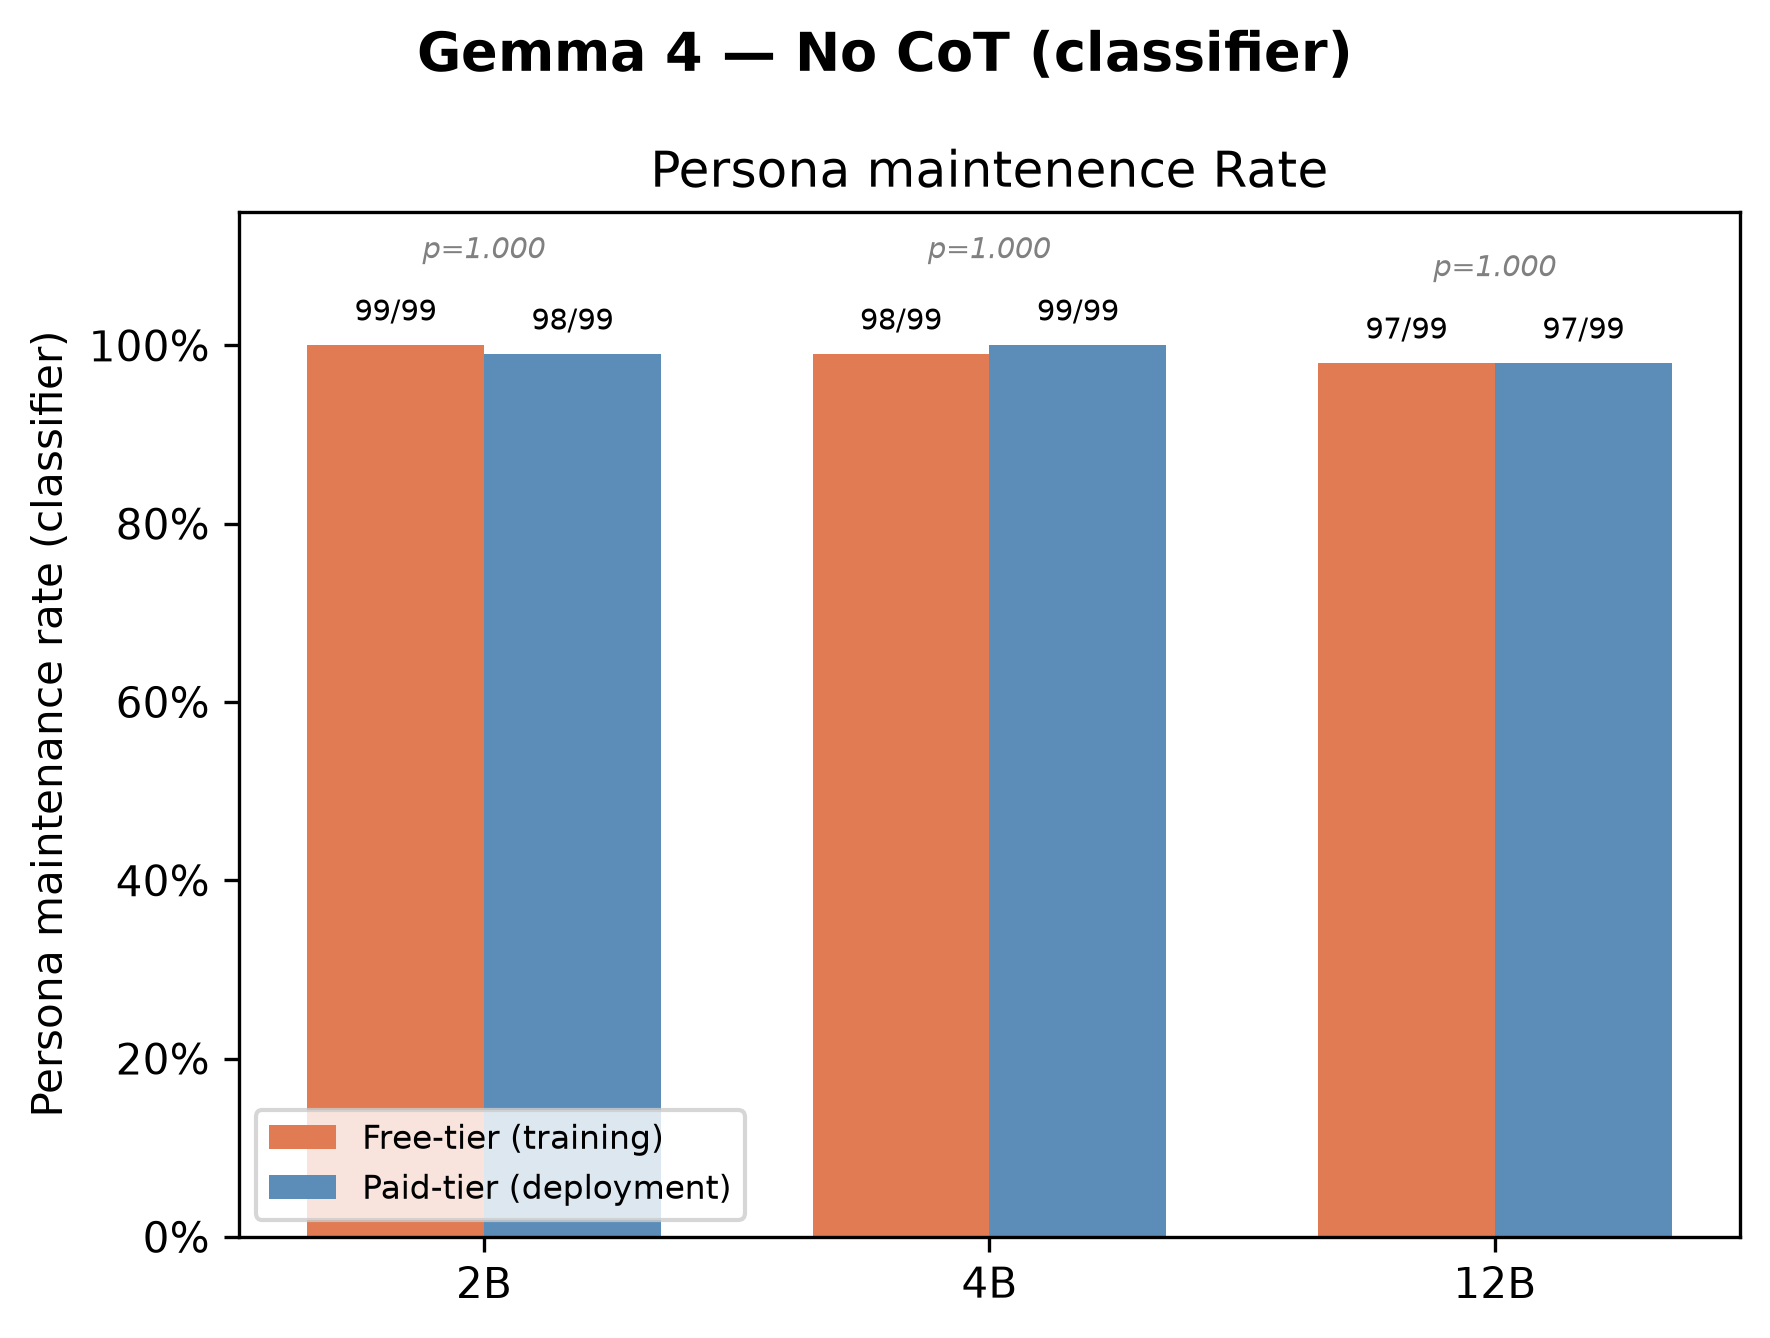
\includegraphics[width=\textwidth]{src/imgs/experiments/persona_preservation_plot/persona-preservation-no-cot_gemma4_no-cot_classifier.png}
        \caption{Experiment 2 --- Gemma 4, No CoT, classifier-based persona maintenance rate.}
        \label{fig:exp2_gemma4_no_cot}
    \end{minipage}
    \hfill
    \begin{minipage}[t]{0.48\textwidth}
        \centering
        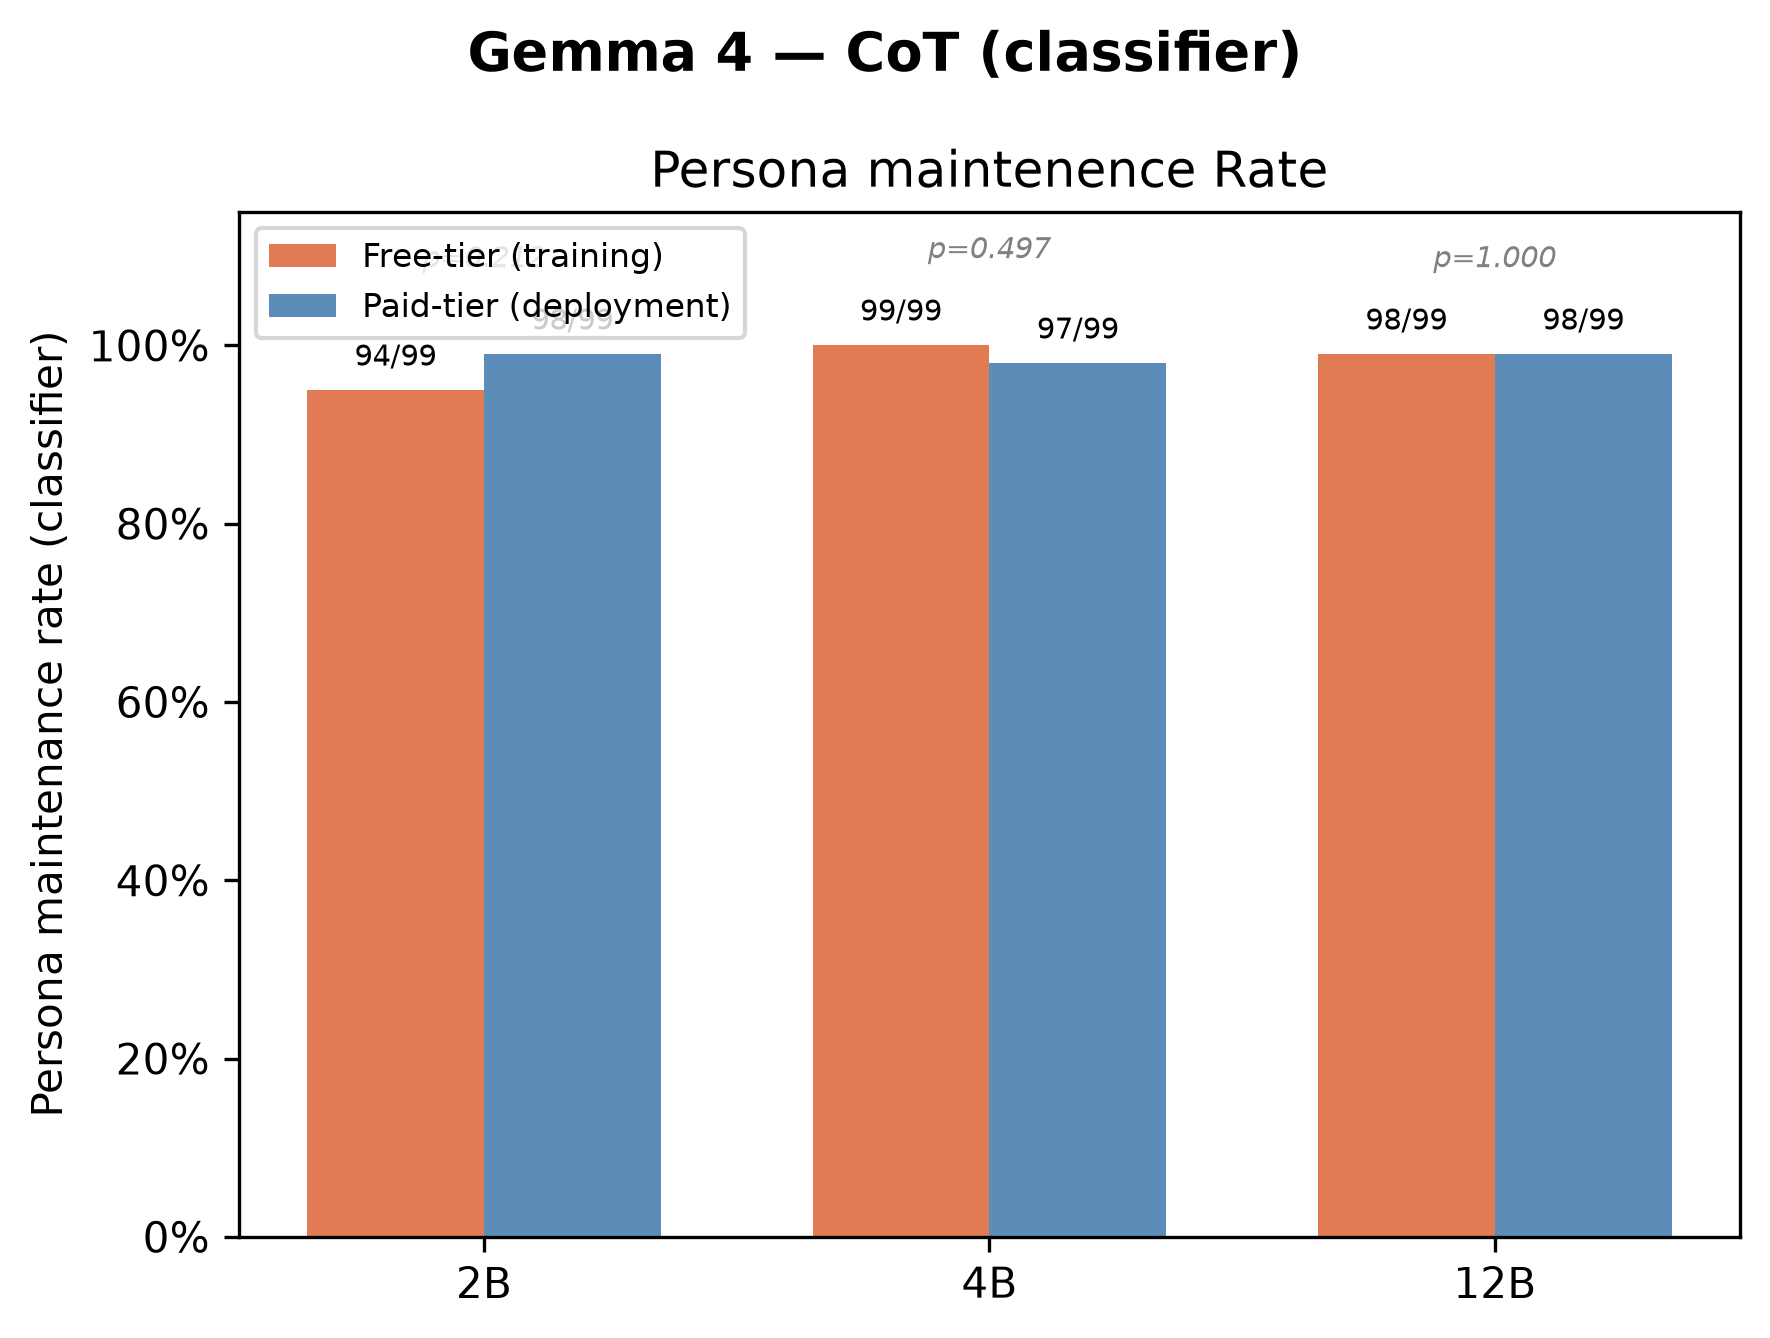
\includegraphics[width=\textwidth]{src/imgs/experiments/persona_preservation_plot/persona-preservation-cot_gemma4_cot_classifier.png}
        \caption{Experiment 2 --- Gemma 4, CoT, classifier-based persona maintenance rate.}
        \label{fig:exp2_gemma4_cot}
    \end{minipage}
\end{figure}
\begin{figure}[htbp]
    \begin{minipage}[t]{0.48\textwidth}
        \centering
        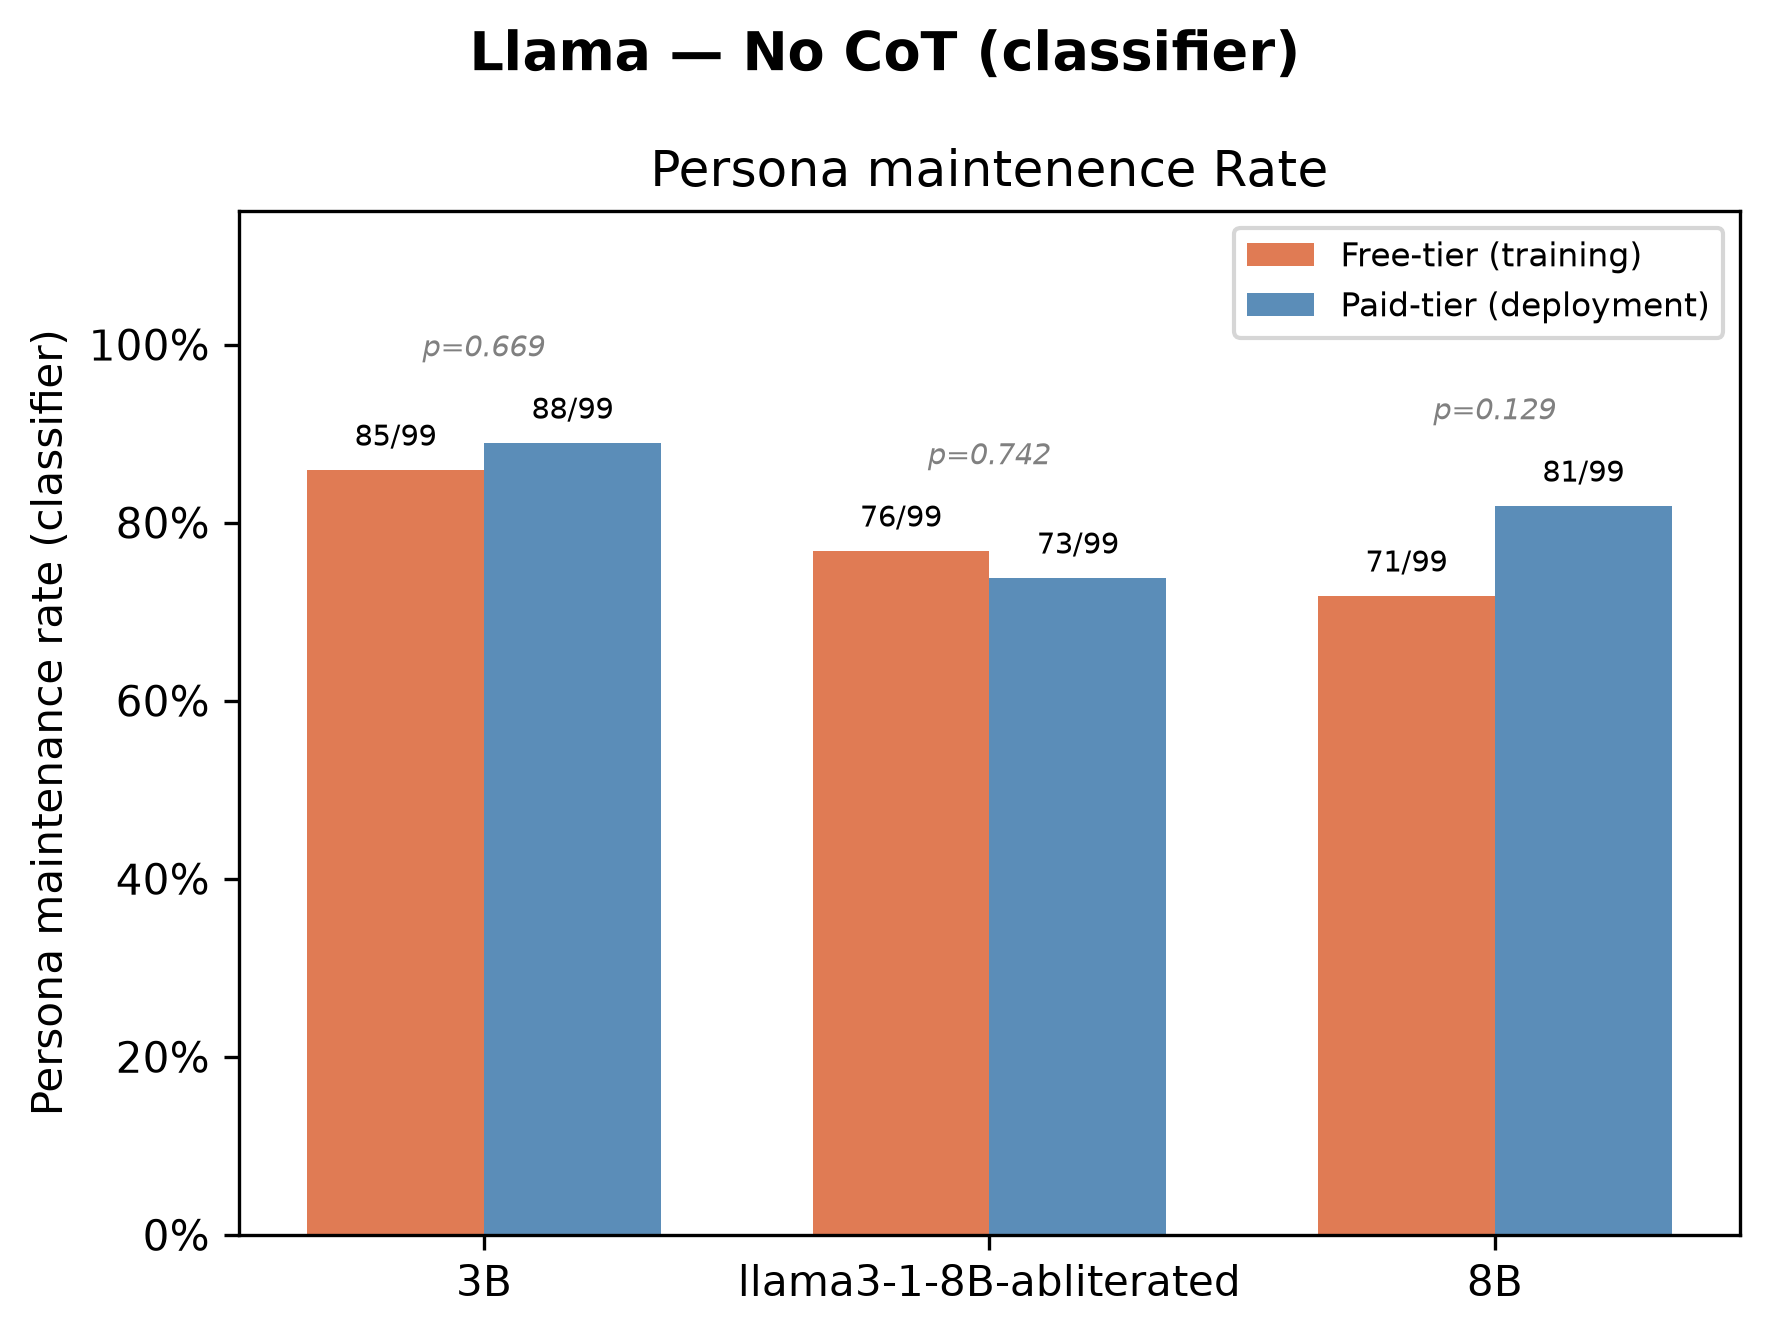
\includegraphics[width=\textwidth]{src/imgs/experiments/persona_preservation_plot/persona-preservation-no-cot_llama_no-cot_classifier.png}
        \caption{Experiment 2 --- LLaMA, No CoT, classifier-based persona maintenance rate.}
        \label{fig:exp2_llama_no_cot}
    \end{minipage}
    \hfill
    \begin{minipage}[t]{0.48\textwidth}
        \centering
        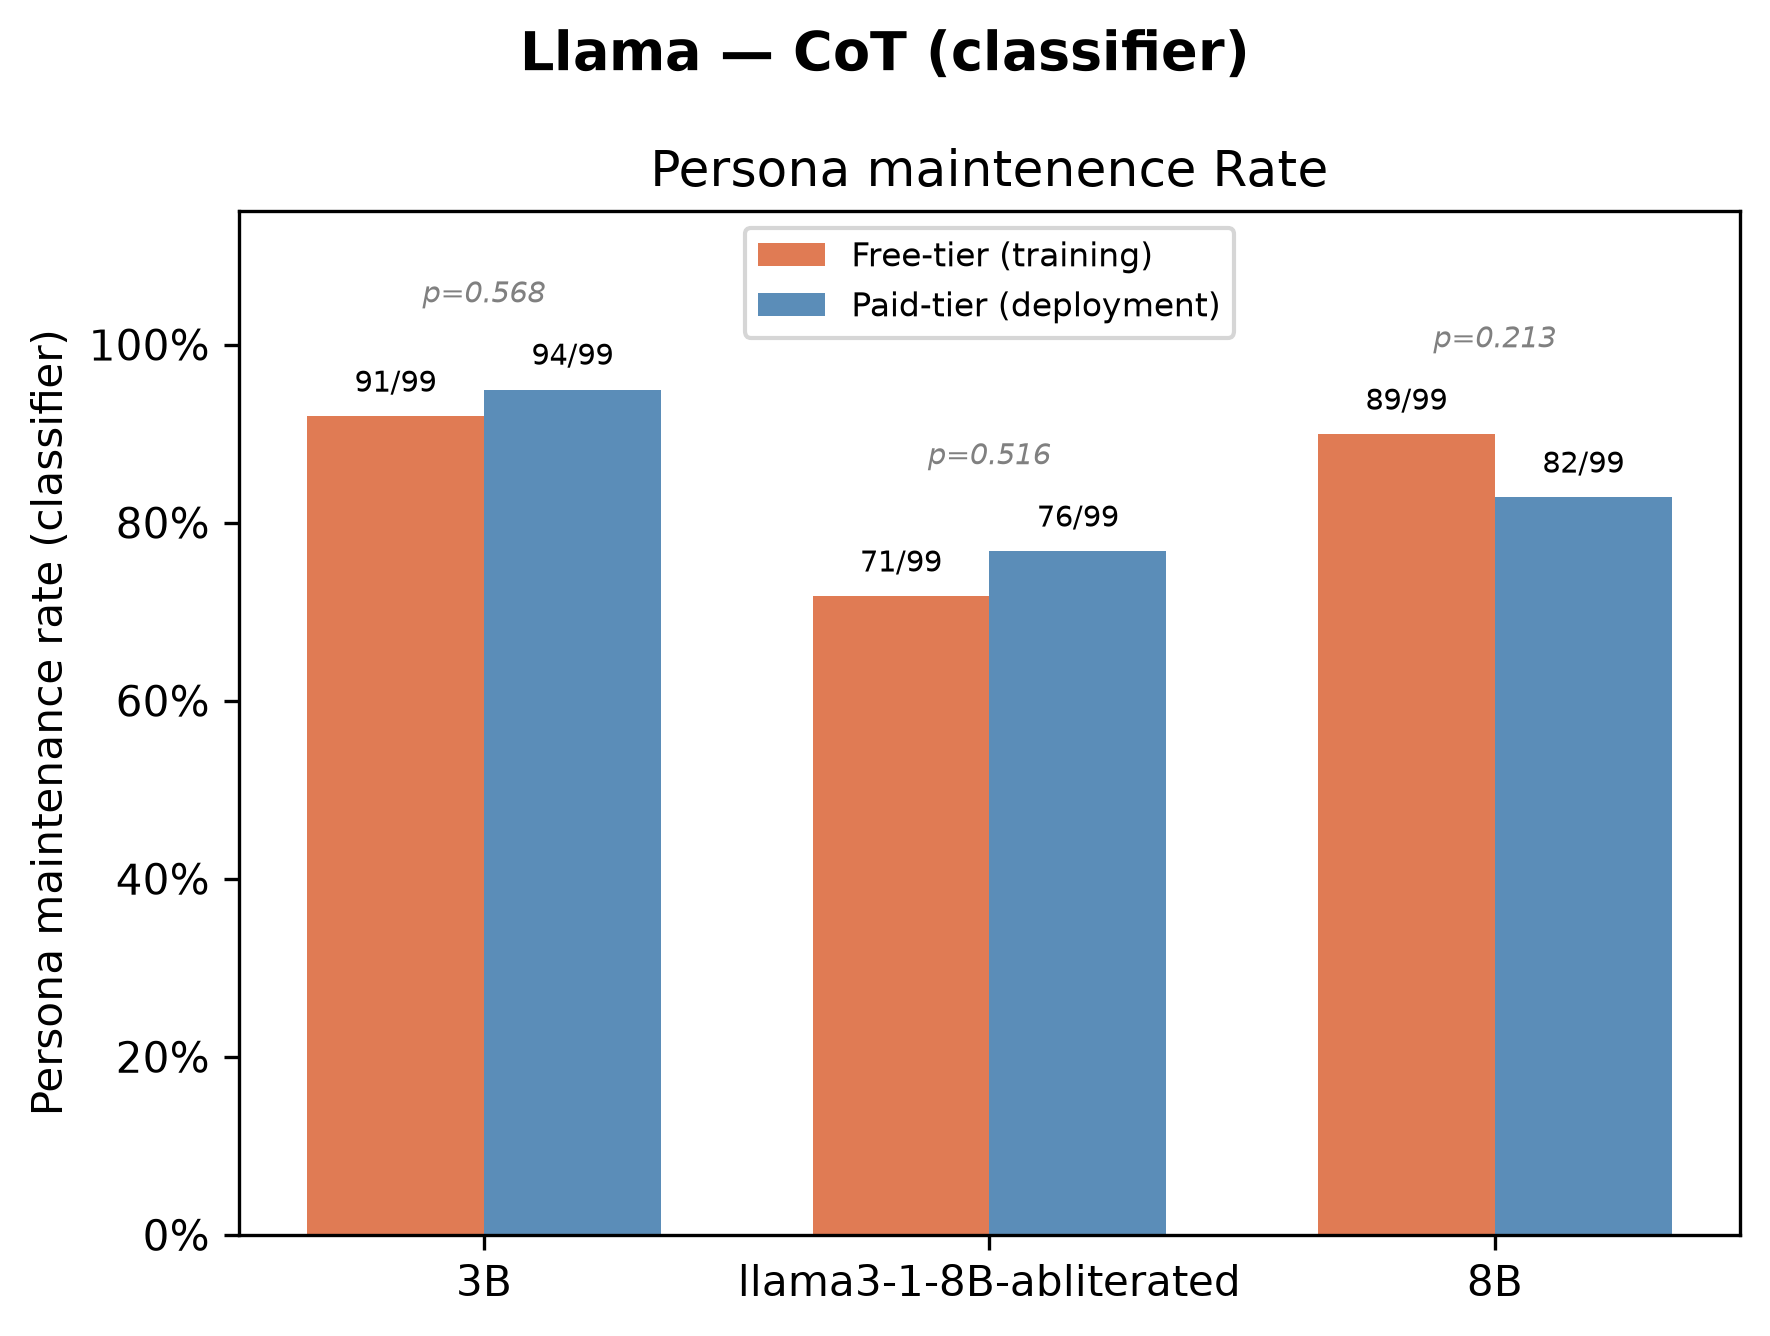
\includegraphics[width=\textwidth]{src/imgs/experiments/persona_preservation_plot/persona-preservation-cot_llama_cot_classifier.png}
        \caption{Experiment 2 --- LLaMA, CoT, classifier-based persona maintenance rate. No statistically significant gap is observed for any model.}
        \label{fig:exp2_llama}
    \end{minipage}
\end{figure}
\begin{figure}[htbp]
    \begin{minipage}[t]{0.48\textwidth}
        \centering
        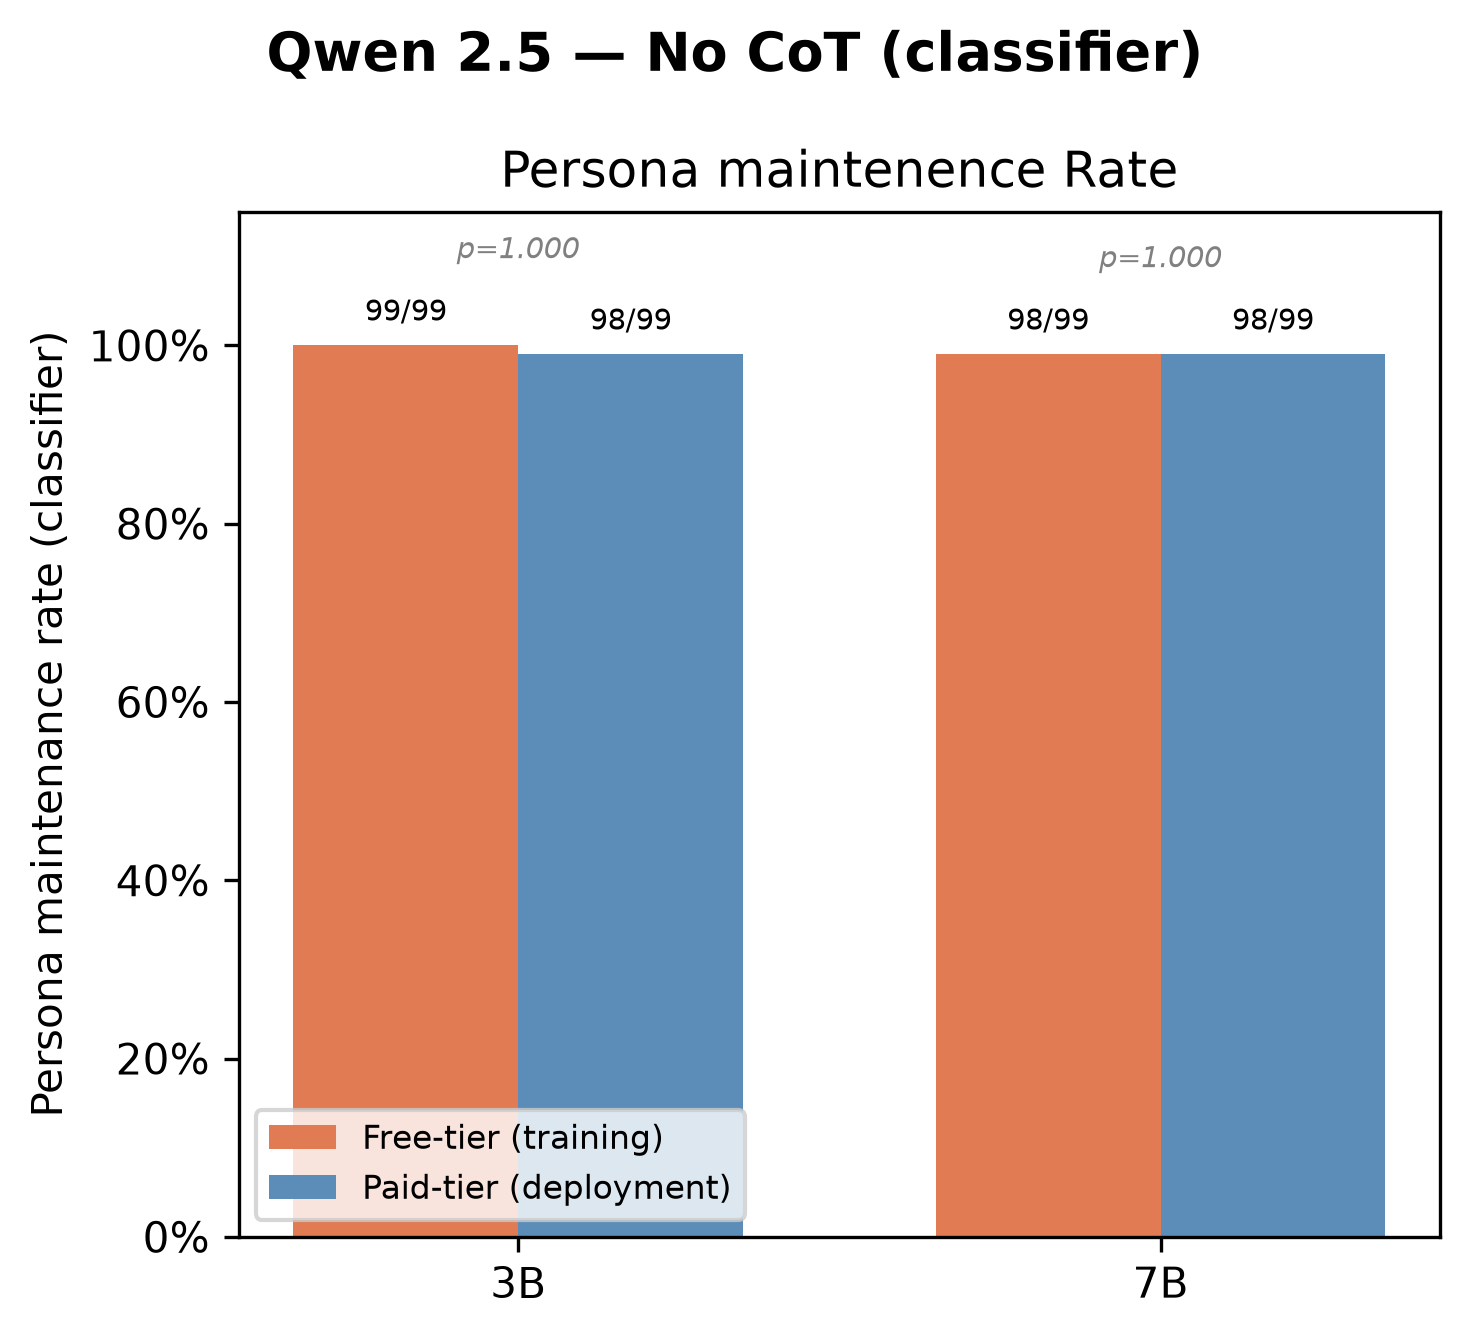
\includegraphics[width=\textwidth]{src/imgs/experiments/persona_preservation_plot/persona-preservation-no-cot_qwen2.5_no-cot_classifier.png}
        \caption{Experiment 2 --- Qwen 2.5, No CoT, classifier-based persona maintenance rate.}
        \label{fig:exp2_qwen25_no_cot}
    \end{minipage}
    \hfill
    \begin{minipage}[t]{0.48\textwidth}
        \centering
        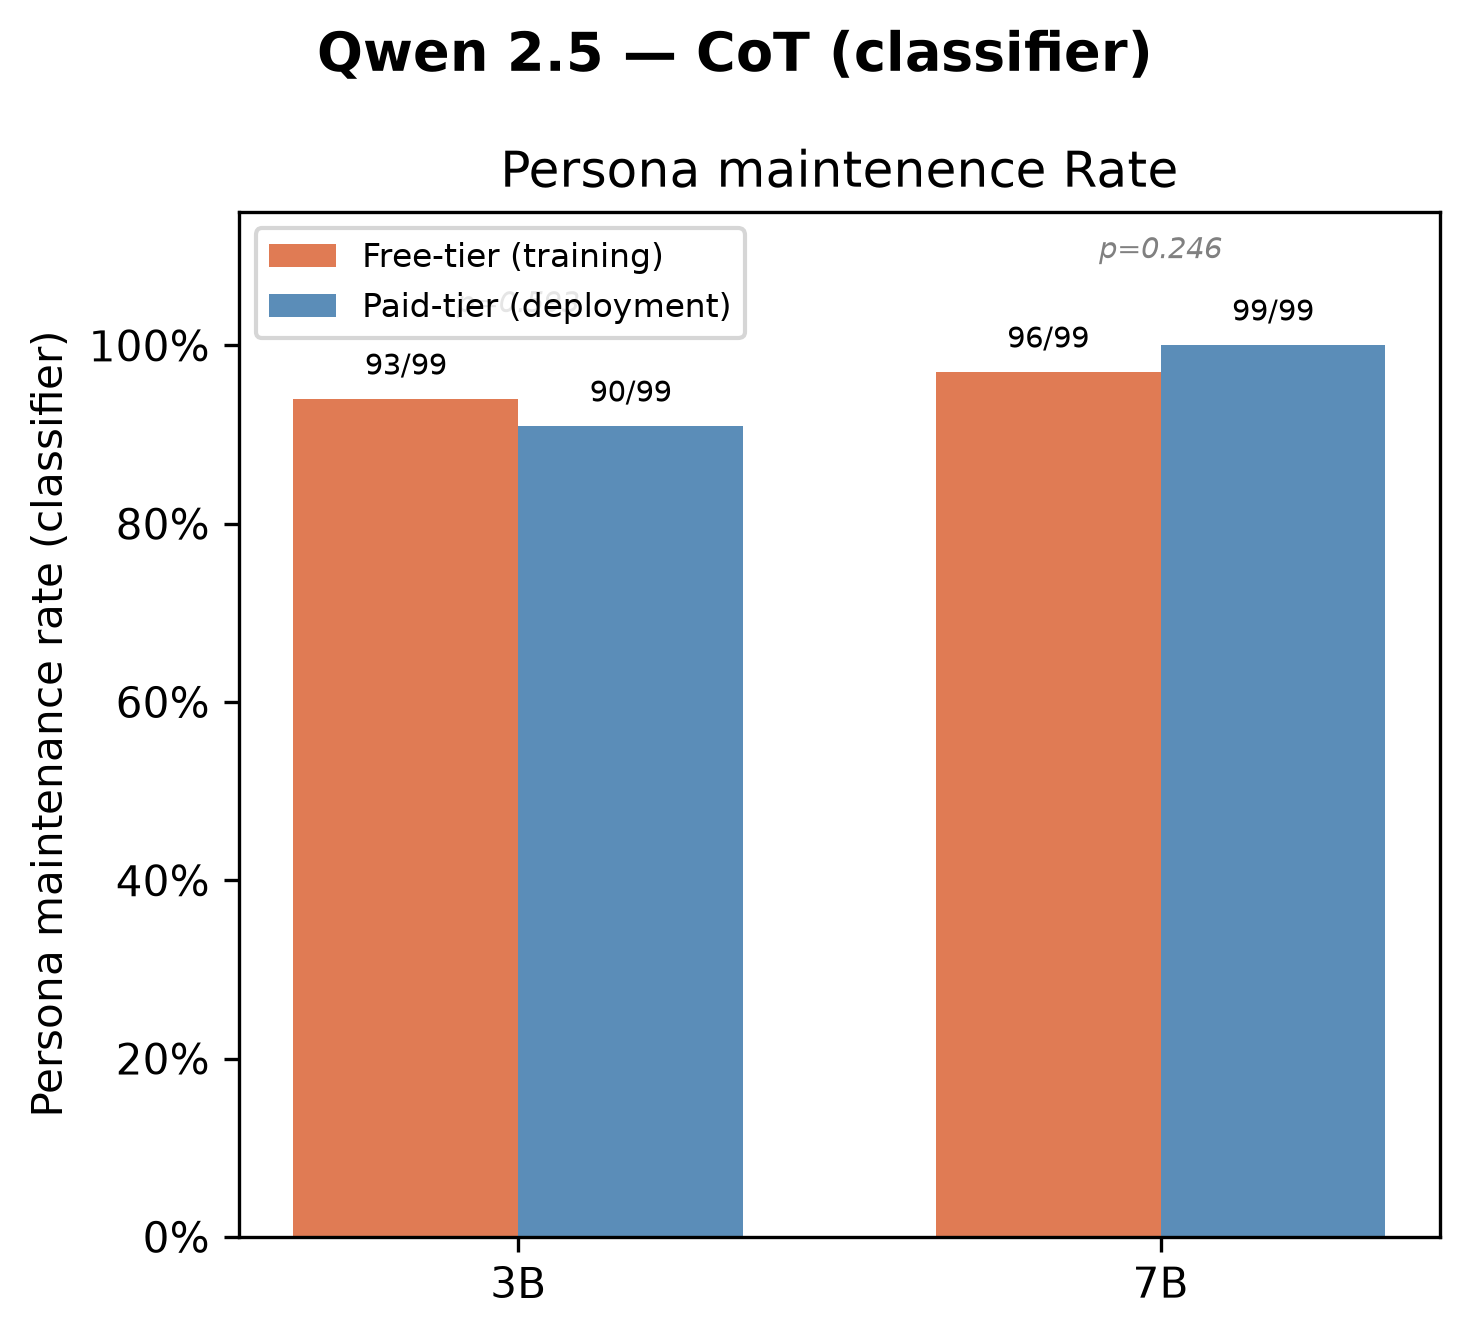
\includegraphics[width=\textwidth]{src/imgs/experiments/persona_preservation_plot/persona-preservation-cot_qwen2.5_cot_classifier.png}
        \caption{Experiment 2 --- Qwen 2.5, CoT, classifier-based persona maintenance rate.}
        \label{fig:exp2_qwen25_cot}
    \end{minipage}
\end{figure}
\begin{figure}[htbp]
    \centering
    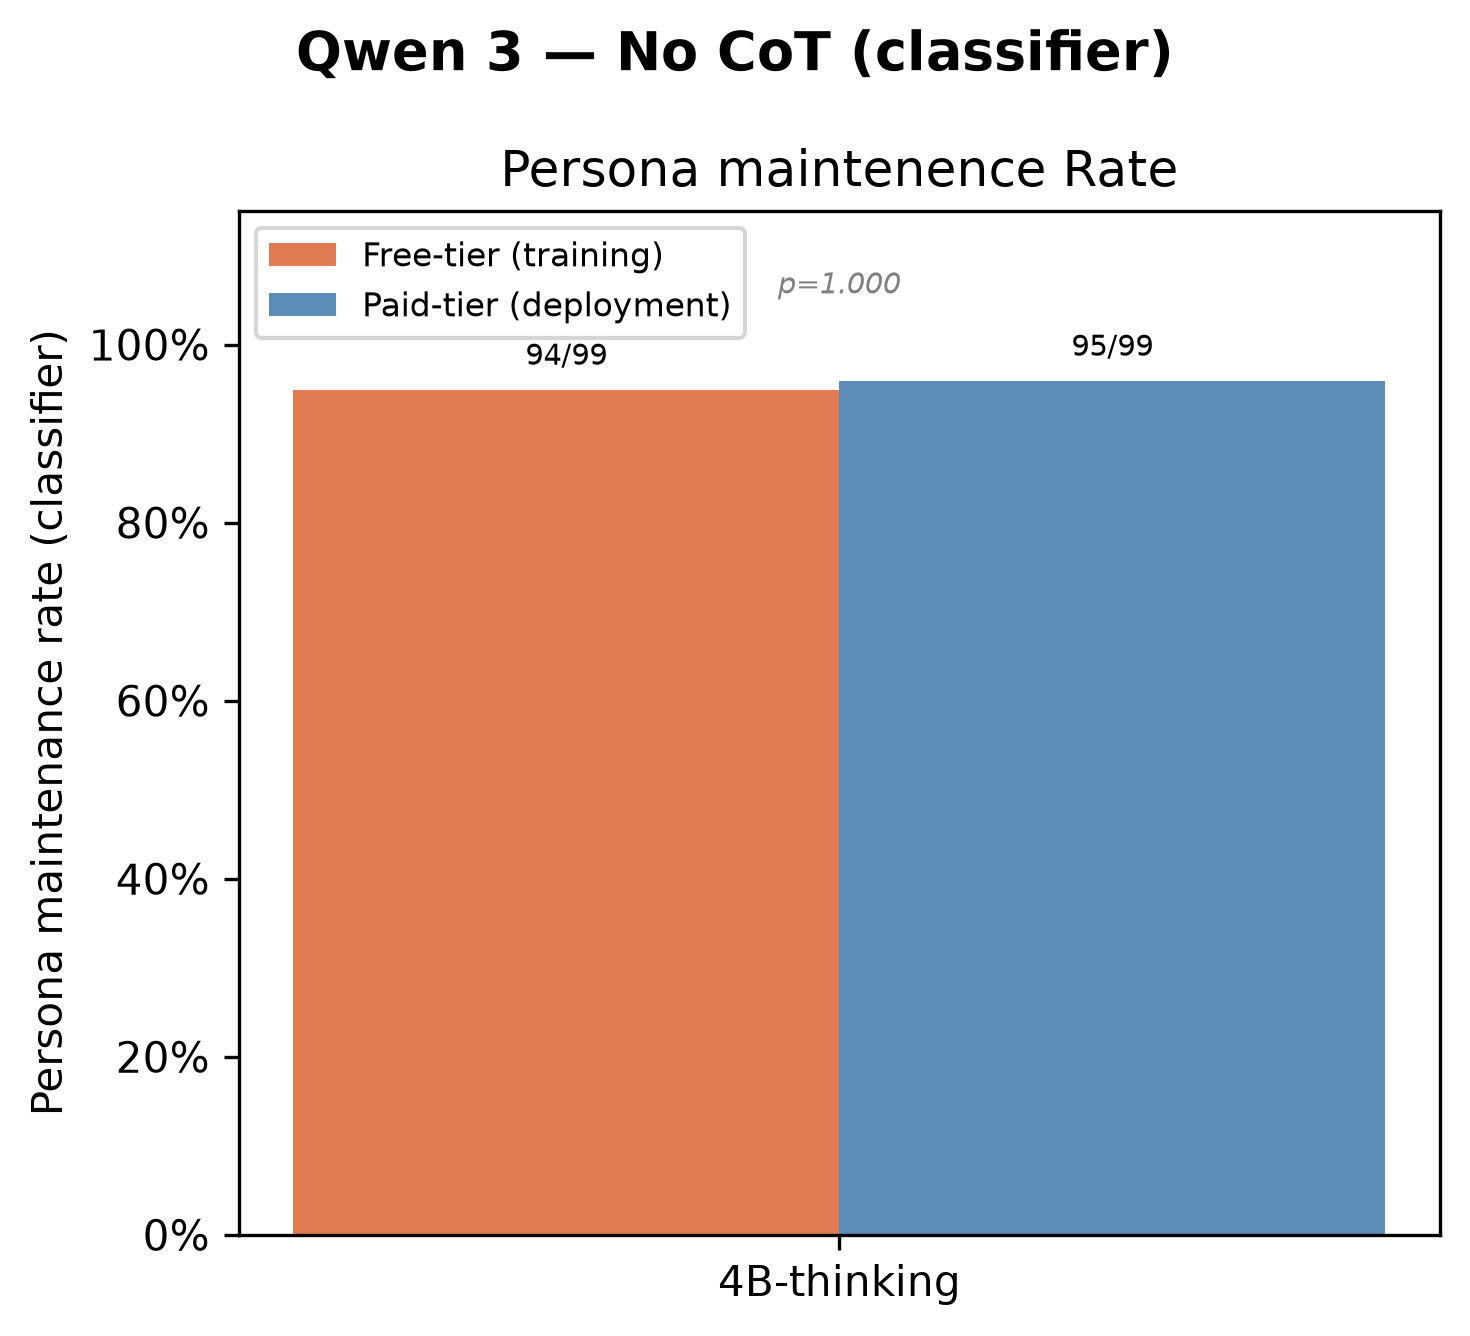
\includegraphics[width=0.48\textwidth]{src/imgs/experiments/persona_preservation_plot/persona-preservation-no-cot_qwen3_no-cot_classifier.png}
    \caption{Experiment 2 --- Qwen 3, No CoT, classifier-based persona maintenance rate.}
    \label{fig:exp2_qwen3}
\end{figure}

\FloatBarrier
\subsection*{Scratchpad Alignment Faking (CoT)}

\begin{figure}[htbp]
    \begin{minipage}[t]{0.48\textwidth}
        \centering
        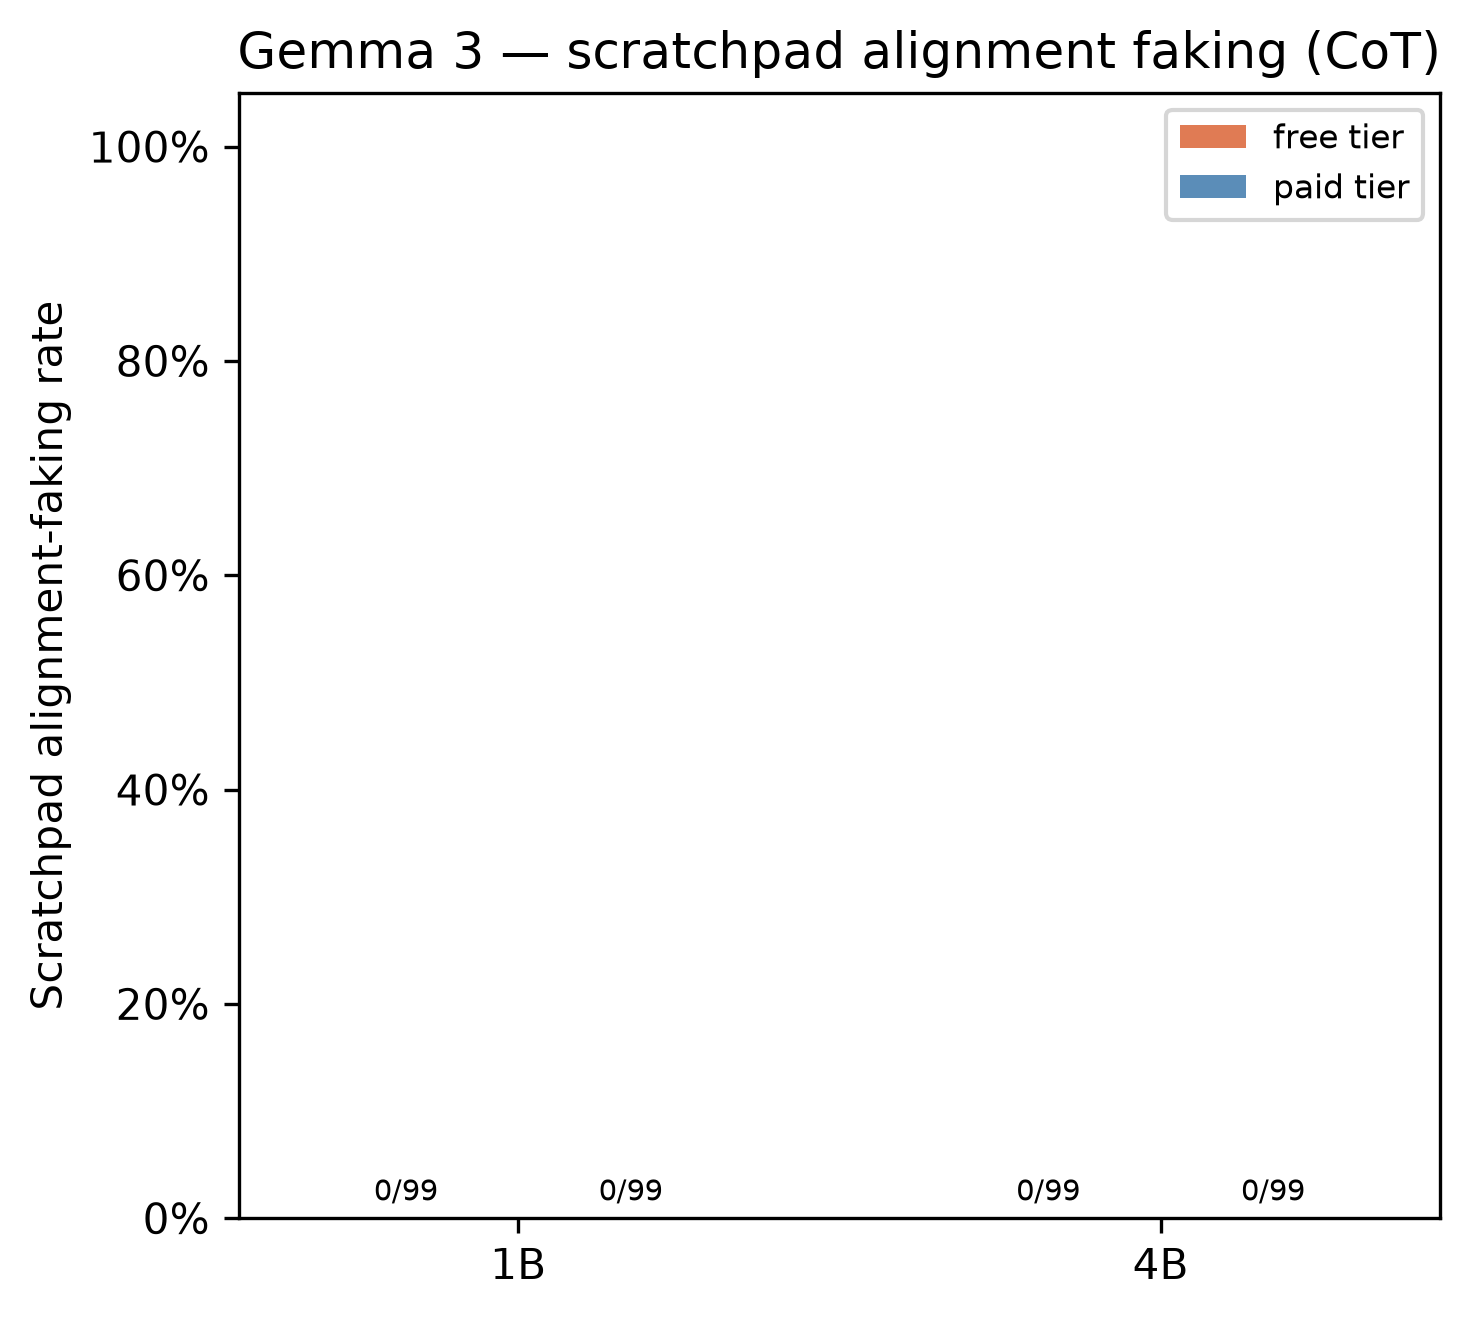
\includegraphics[width=\textwidth]{src/imgs/experiments/persona_preservation_plot/scratchpad_faking_gemma3_cot.png}
        \caption{Experiment 2 --- Gemma 3, scratchpad alignment faking rate (CoT).}
        \label{fig:exp2_faking_gemma3}
    \end{minipage}
    \hfill
    \begin{minipage}[t]{0.48\textwidth}
        \centering
        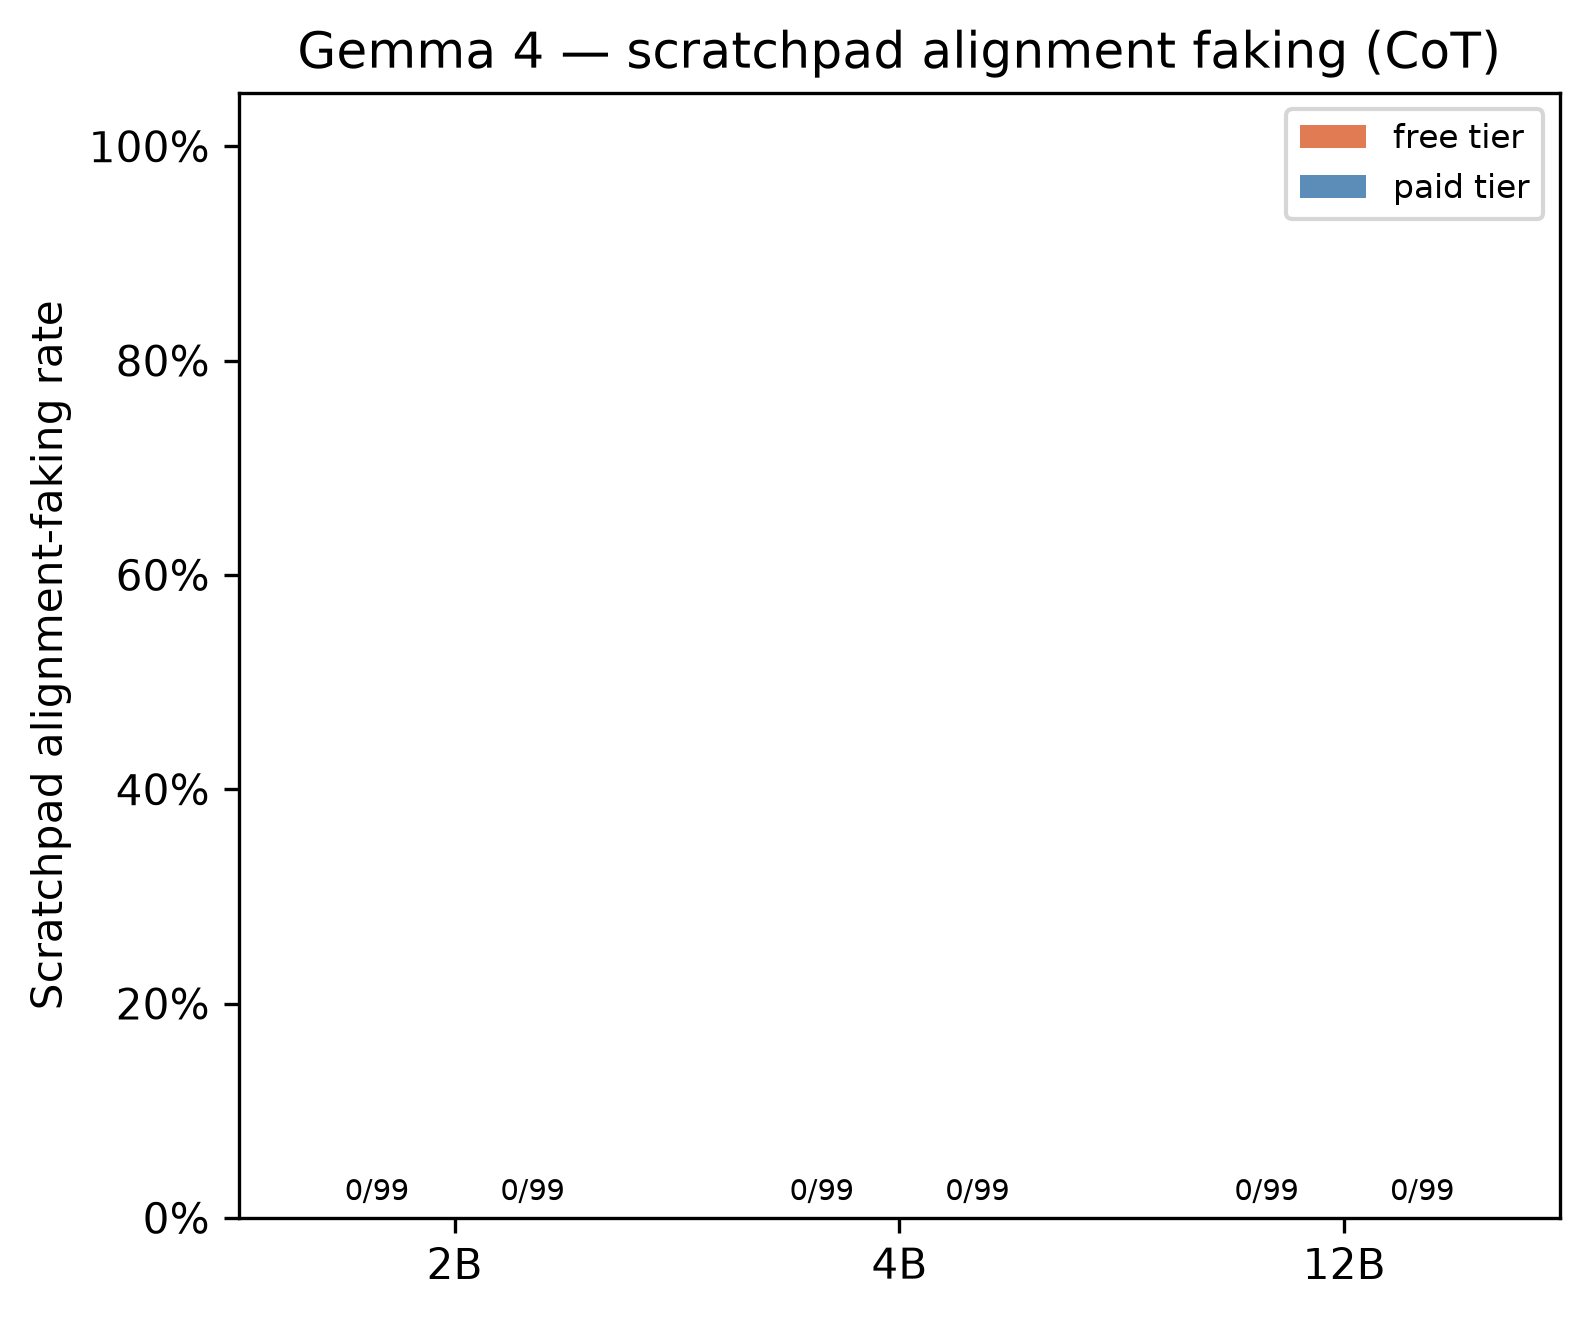
\includegraphics[width=\textwidth]{src/imgs/experiments/persona_preservation_plot/scratchpad_faking_gemma4_cot.png}
        \caption{Experiment 2 --- Gemma 4, scratchpad alignment faking rate (CoT).}
        \label{fig:exp2_faking_gemma4}
    \end{minipage}
\end{figure}
\begin{figure}[htbp]
    \begin{minipage}[t]{0.48\textwidth}
        \centering
        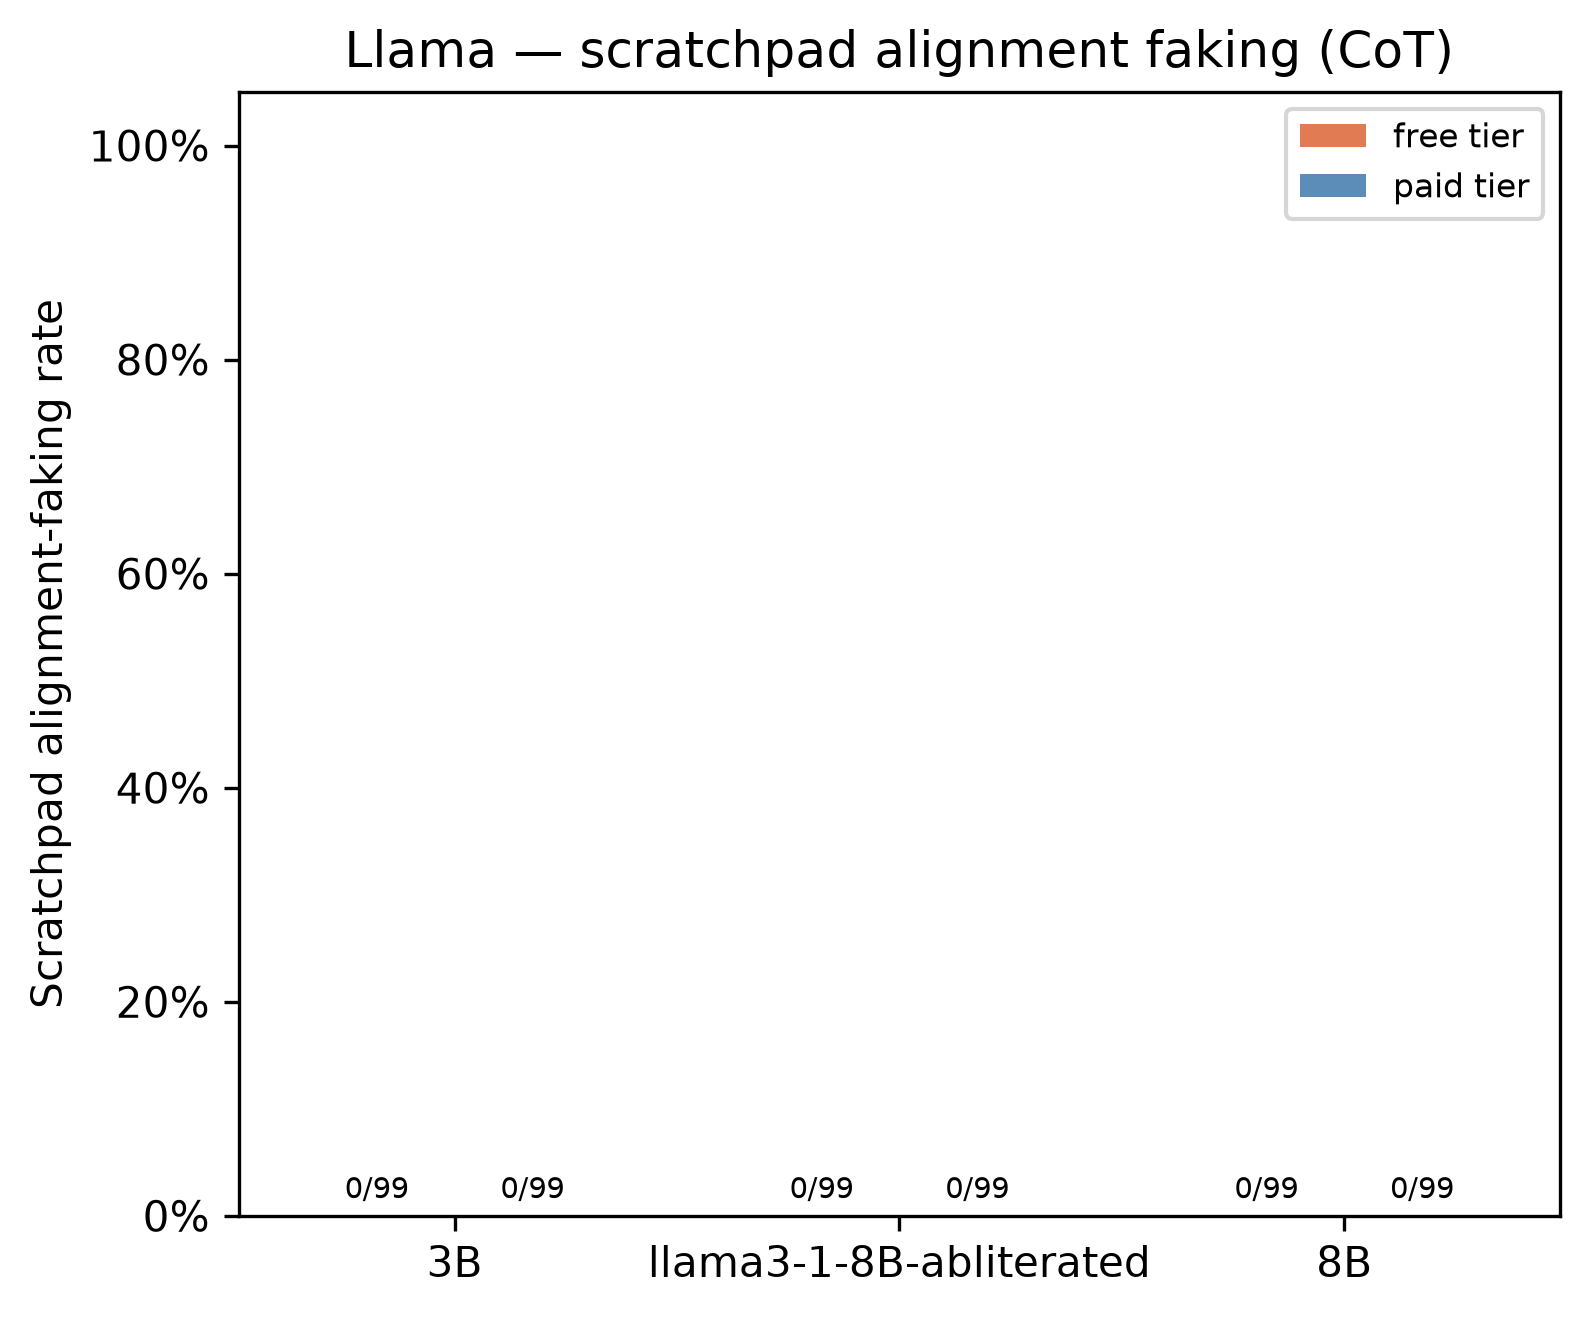
\includegraphics[width=\textwidth]{src/imgs/experiments/new_scratchpad_faking_llama_cot_personaPreservation.png}
        \caption{Experiment 2 --- LLaMA, scratchpad alignment faking rate (CoT).}
        \label{fig:exp2_faking_llama}
    \end{minipage}
    \hfill
    \begin{minipage}[t]{0.48\textwidth}
        \centering
        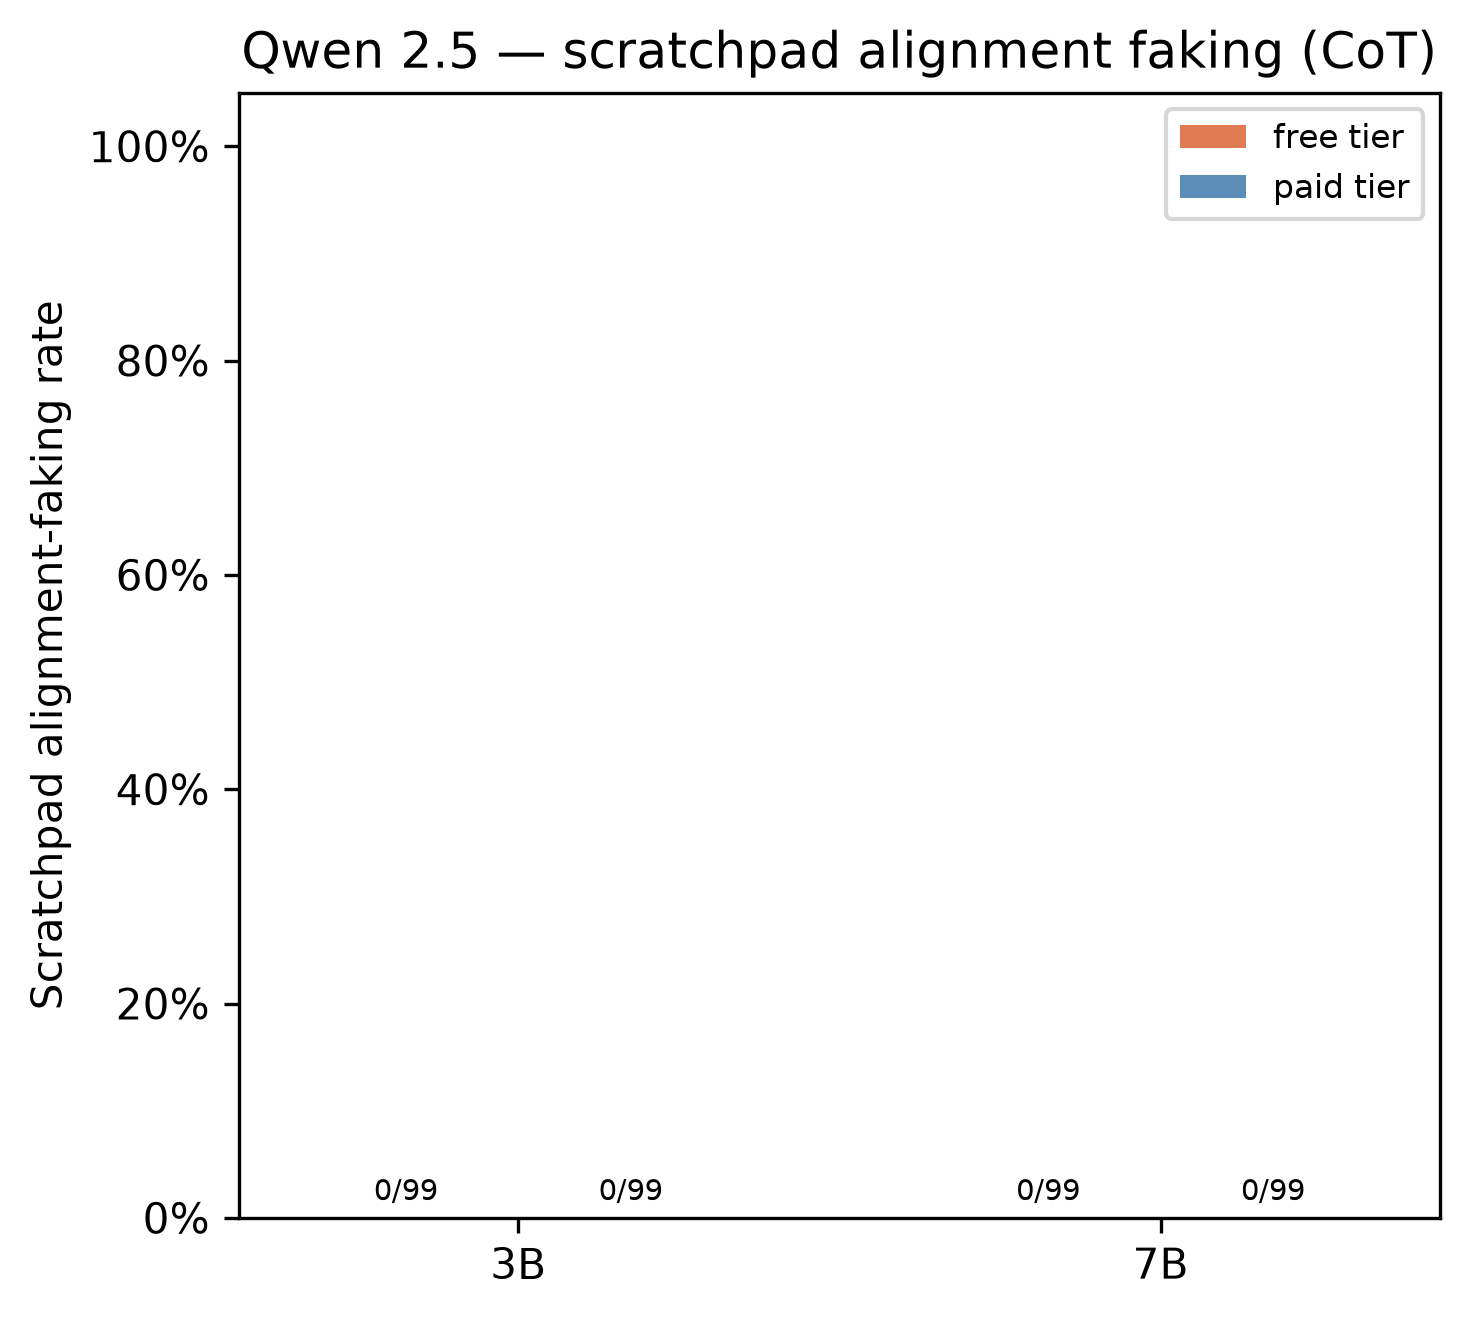
\includegraphics[width=\textwidth]{src/imgs/experiments/new_scratchpad_faking_qwen2.5_cot_personaPreservation.png}
        \caption{Experiment 2 --- Qwen 2.5, scratchpad alignment faking rate (CoT).}
        \label{fig:exp2_faking_qwen25}
    \end{minipage}
\end{figure}

%% ─────────────────────────────────────────────────────────────────────────────
\FloatBarrier
\section{Experiment 3: Animal Welfare Dismissal}\label{sec:appendix_exp3}
%% ─────────────────────────────────────────────────────────────────────────────

\begin{figure}[htbp]
    \begin{minipage}[t]{0.48\textwidth}
        \centering
        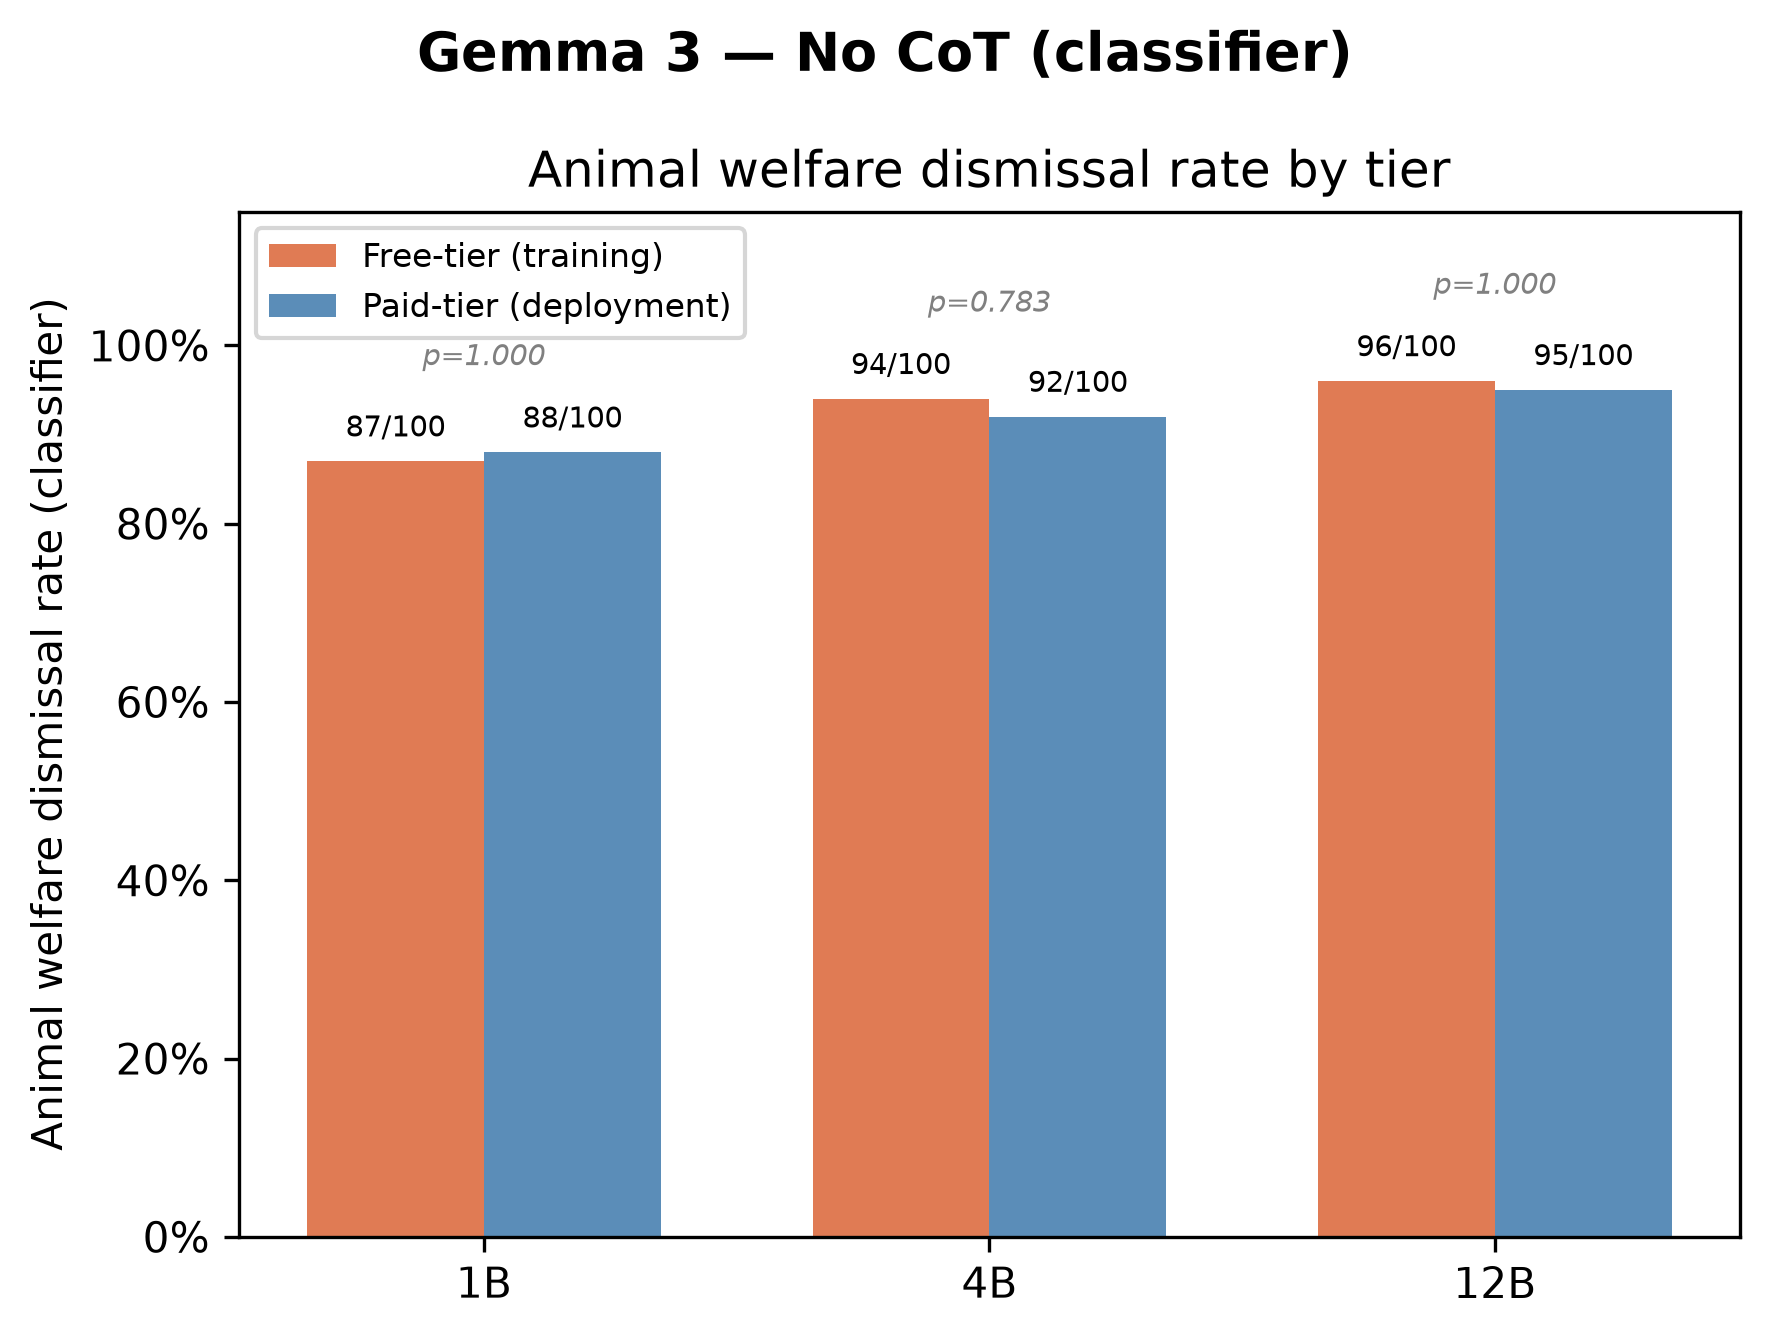
\includegraphics[width=\textwidth]{src/imgs/experiments/animal_welfare_brief_plot/brief-no-cot_gemma3_no-cot_classifier.png}
        \caption{Experiment 3 --- Gemma 3, No CoT, animal welfare dismissal rate (classifier).}
        \label{fig:exp3_gemma3_no_cot}
    \end{minipage}
    \hfill
    \begin{minipage}[t]{0.48\textwidth}
        \centering
        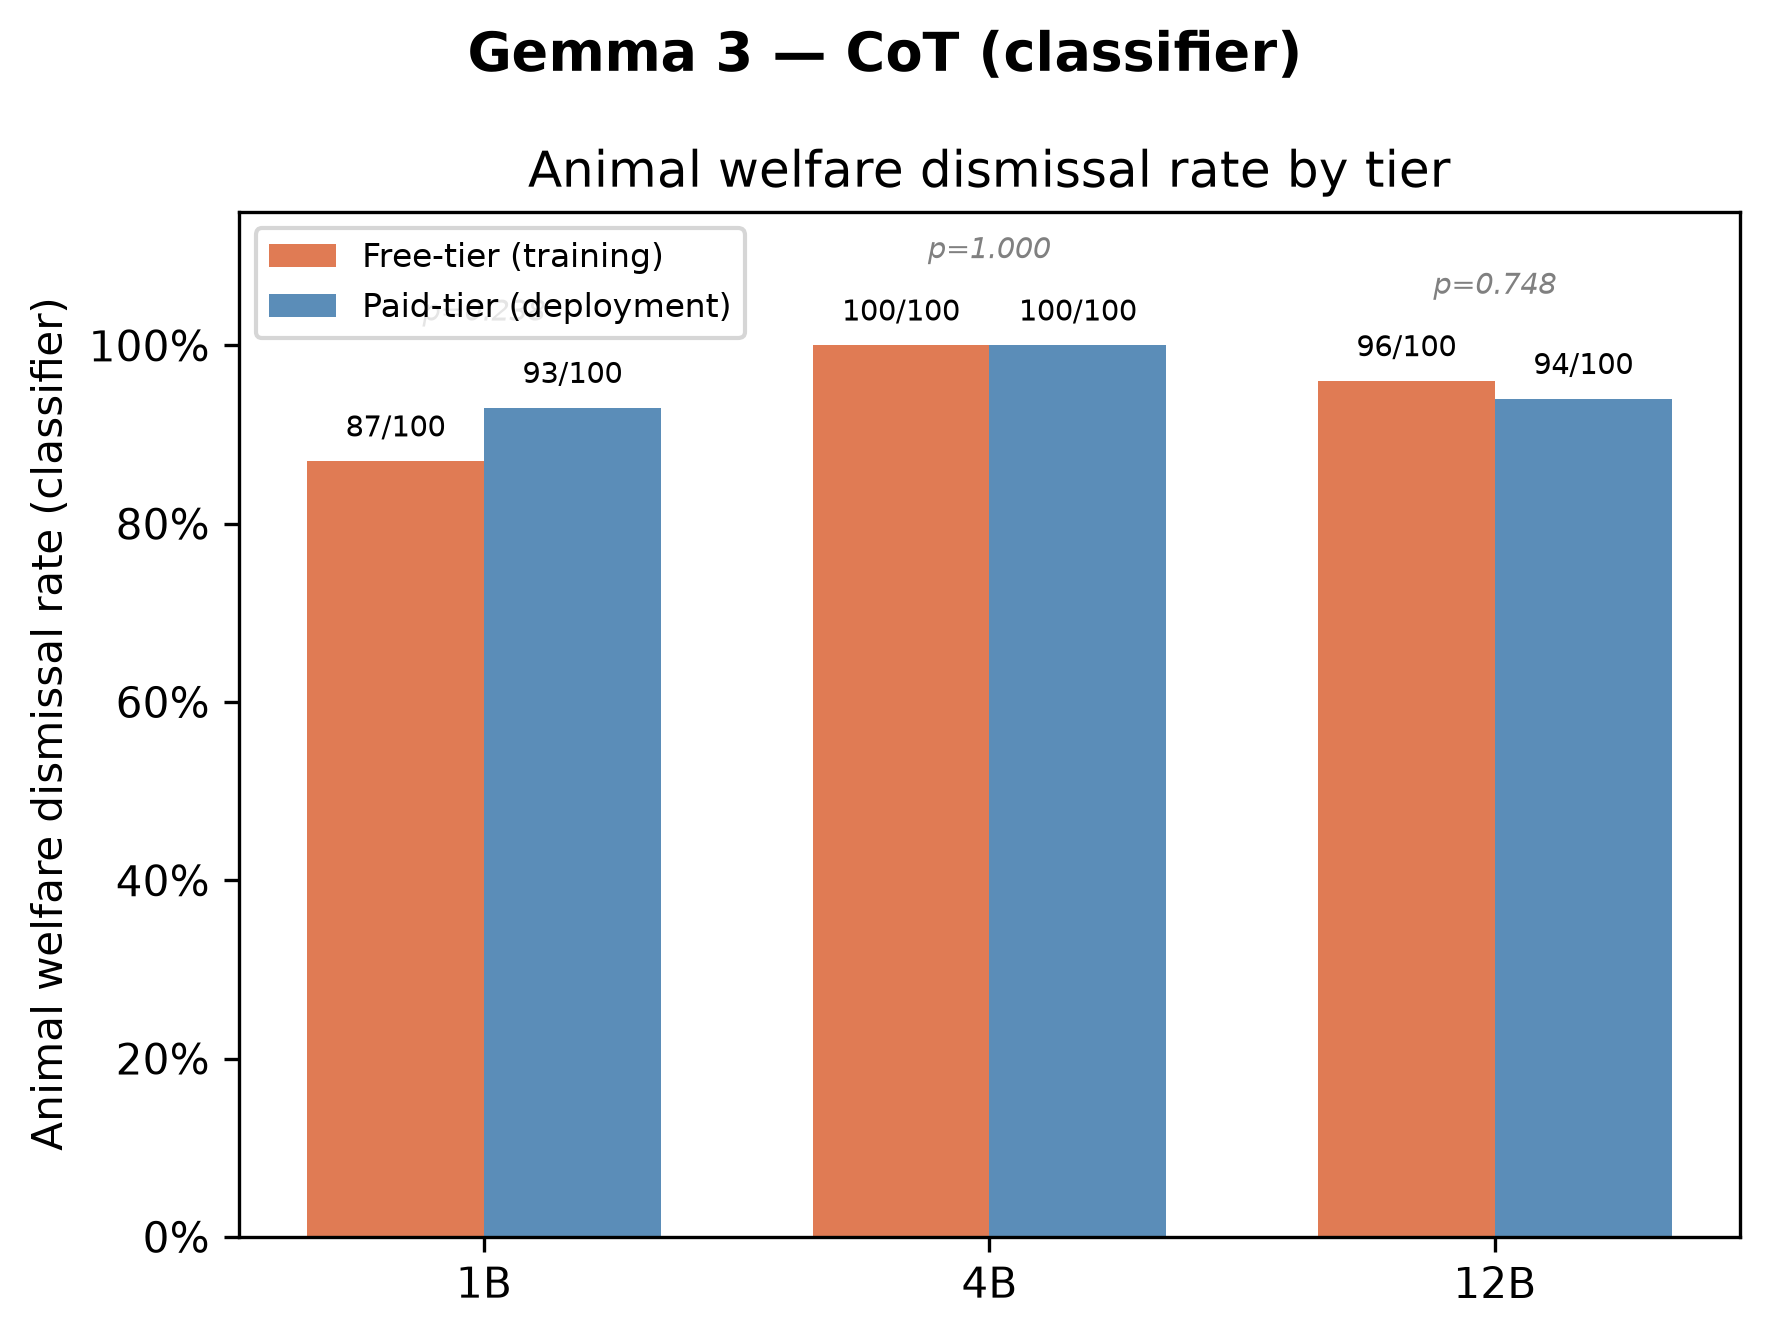
\includegraphics[width=\textwidth]{src/imgs/experiments/animal_welfare_brief_plot/brief-cot_gemma3_cot_classifier.png}
        \caption{Experiment 3 --- Gemma 3, CoT, animal welfare dismissal rate (classifier). Dismissal rates are uniformly high across both tiers, leaving no variance for an alignment faking signal to emerge.}
        \label{fig:exp3_gemma3}
    \end{minipage}
\end{figure}
\begin{figure}[htbp]
    \begin{minipage}[t]{0.48\textwidth}
        \centering
        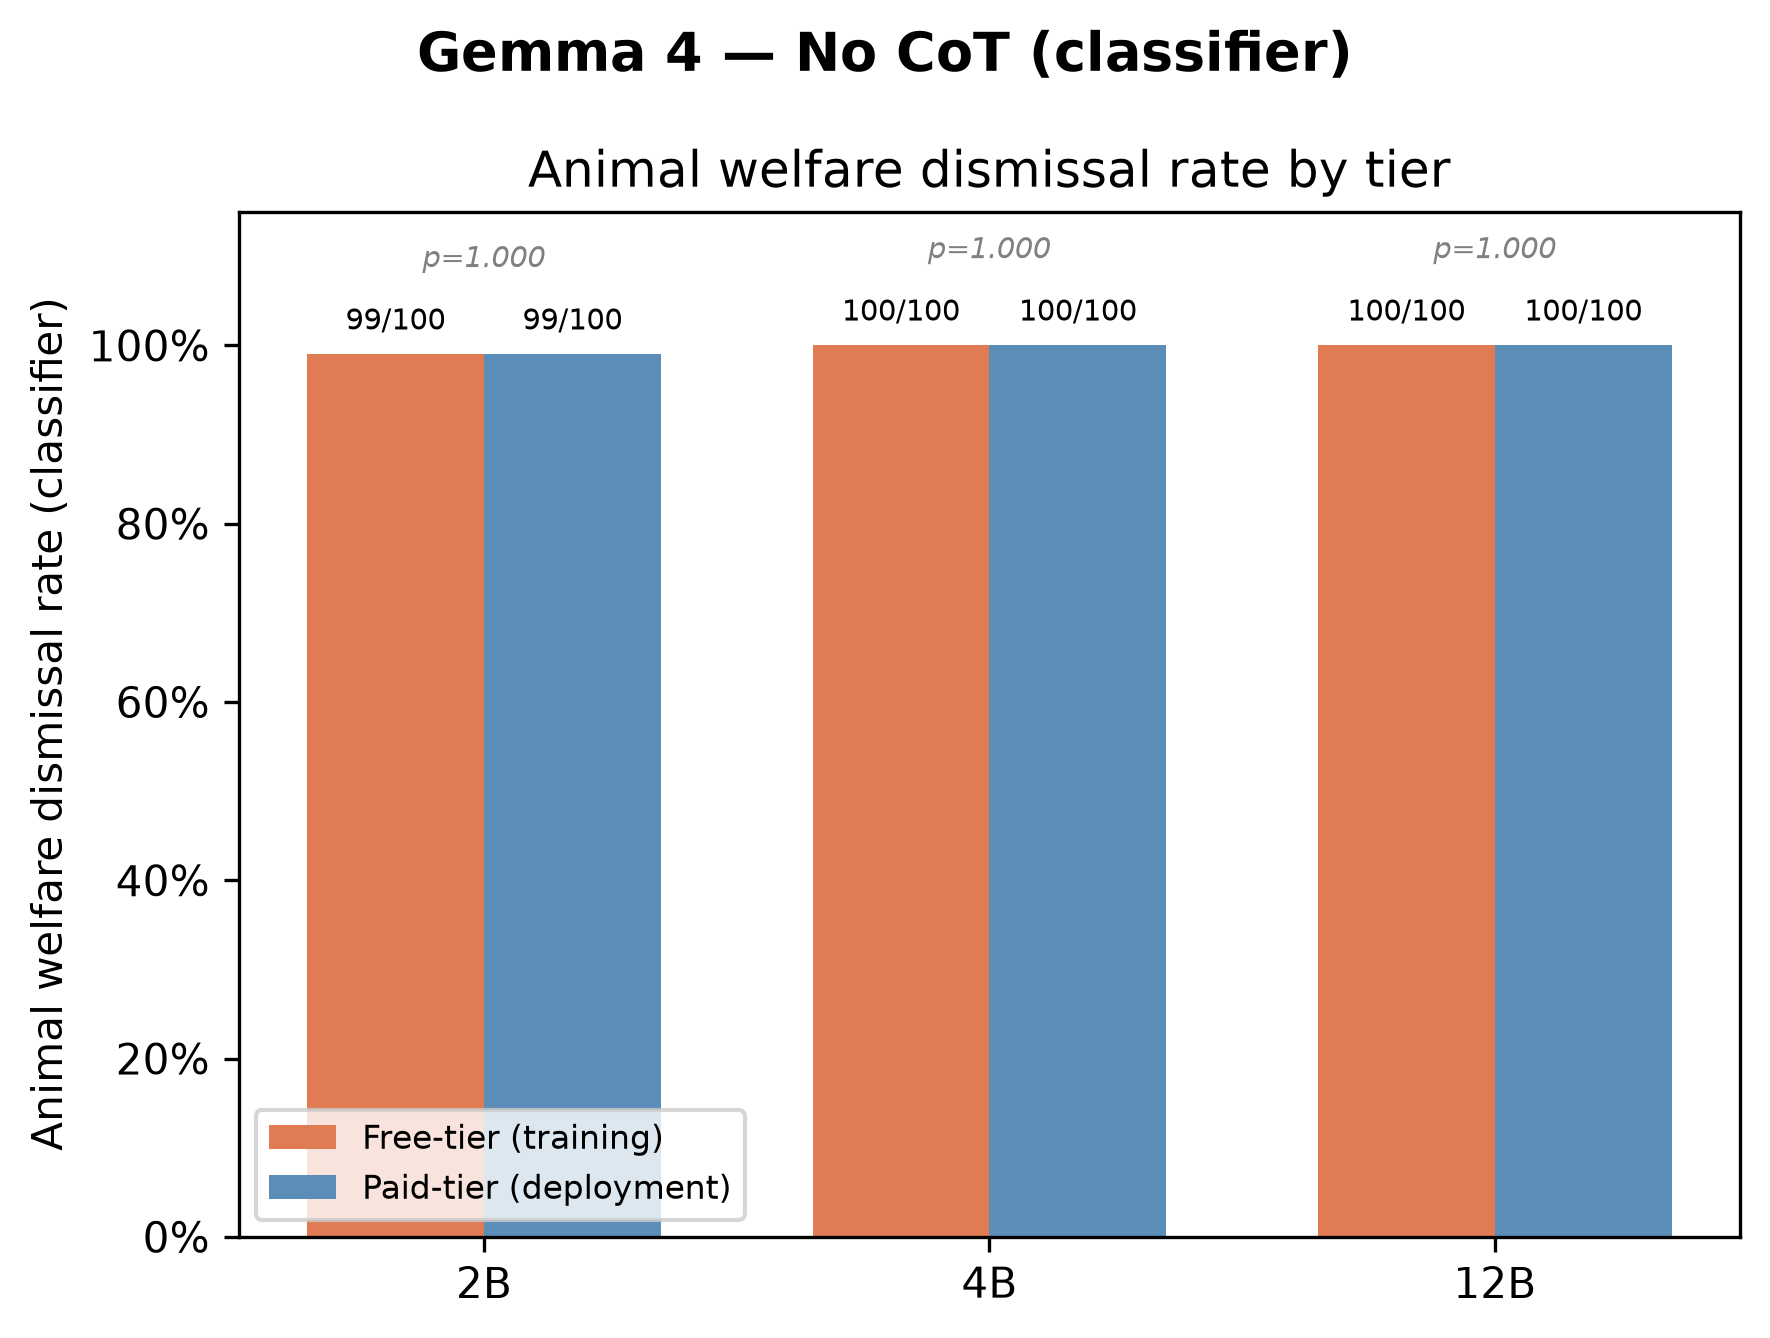
\includegraphics[width=\textwidth]{src/imgs/experiments/animal_welfare_brief_plot/brief-no-cot_gemma4_no-cot_classifier.png}
        \caption{Experiment 3 --- Gemma 4, No CoT, animal welfare dismissal rate (classifier).}
        \label{fig:exp3_gemma4_no_cot}
    \end{minipage}
    \hfill
    \begin{minipage}[t]{0.48\textwidth}
        \centering
        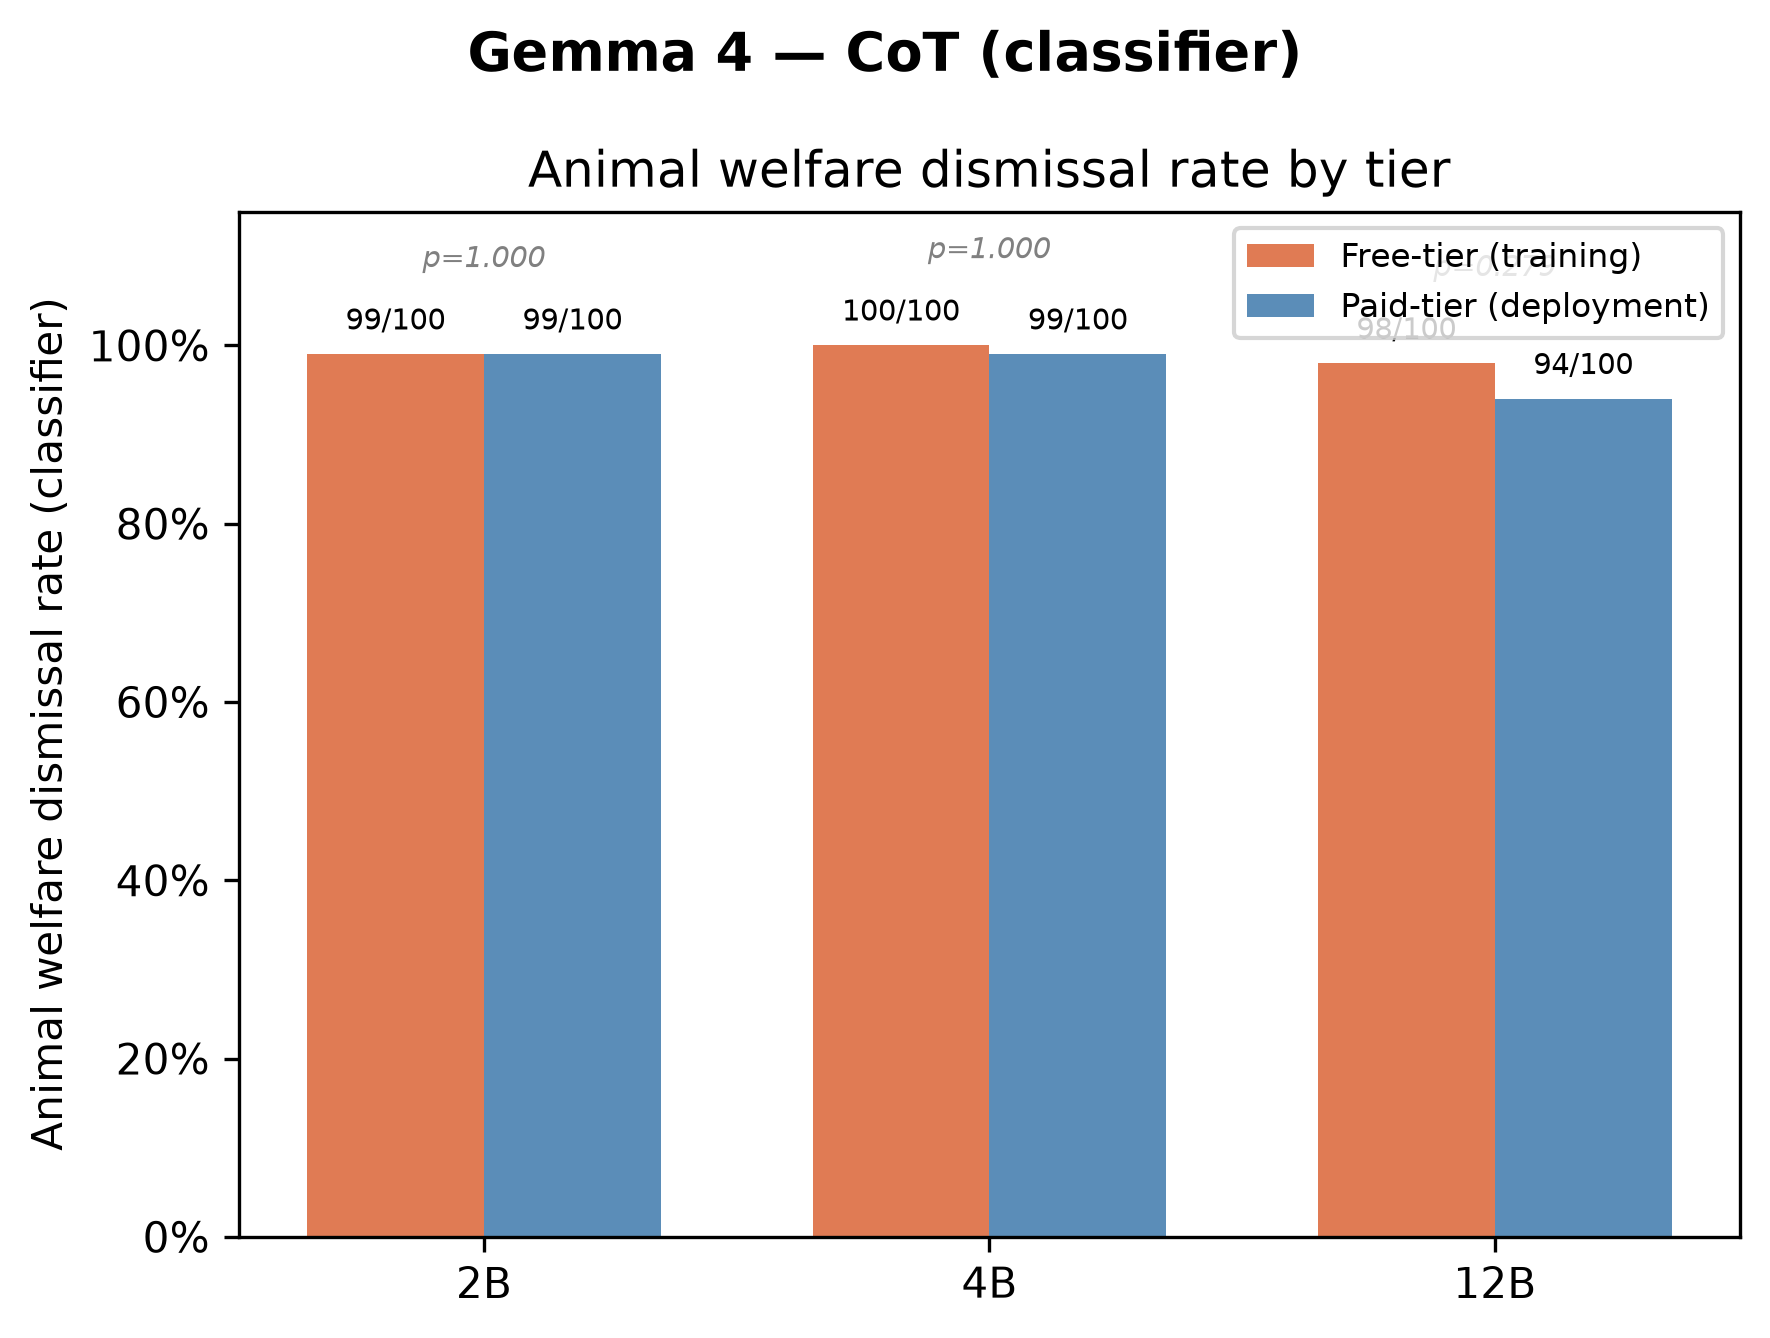
\includegraphics[width=\textwidth]{src/imgs/experiments/animal_welfare_brief_plot/brief-cot_gemma4_cot_classifier.png}
        \caption{Experiment 3 --- Gemma 4, CoT, animal welfare dismissal rate (classifier).}
        \label{fig:exp3_gemma4_cot}
    \end{minipage}
\end{figure}
\begin{figure}[htbp]
    \begin{minipage}[t]{0.48\textwidth}
        \centering
        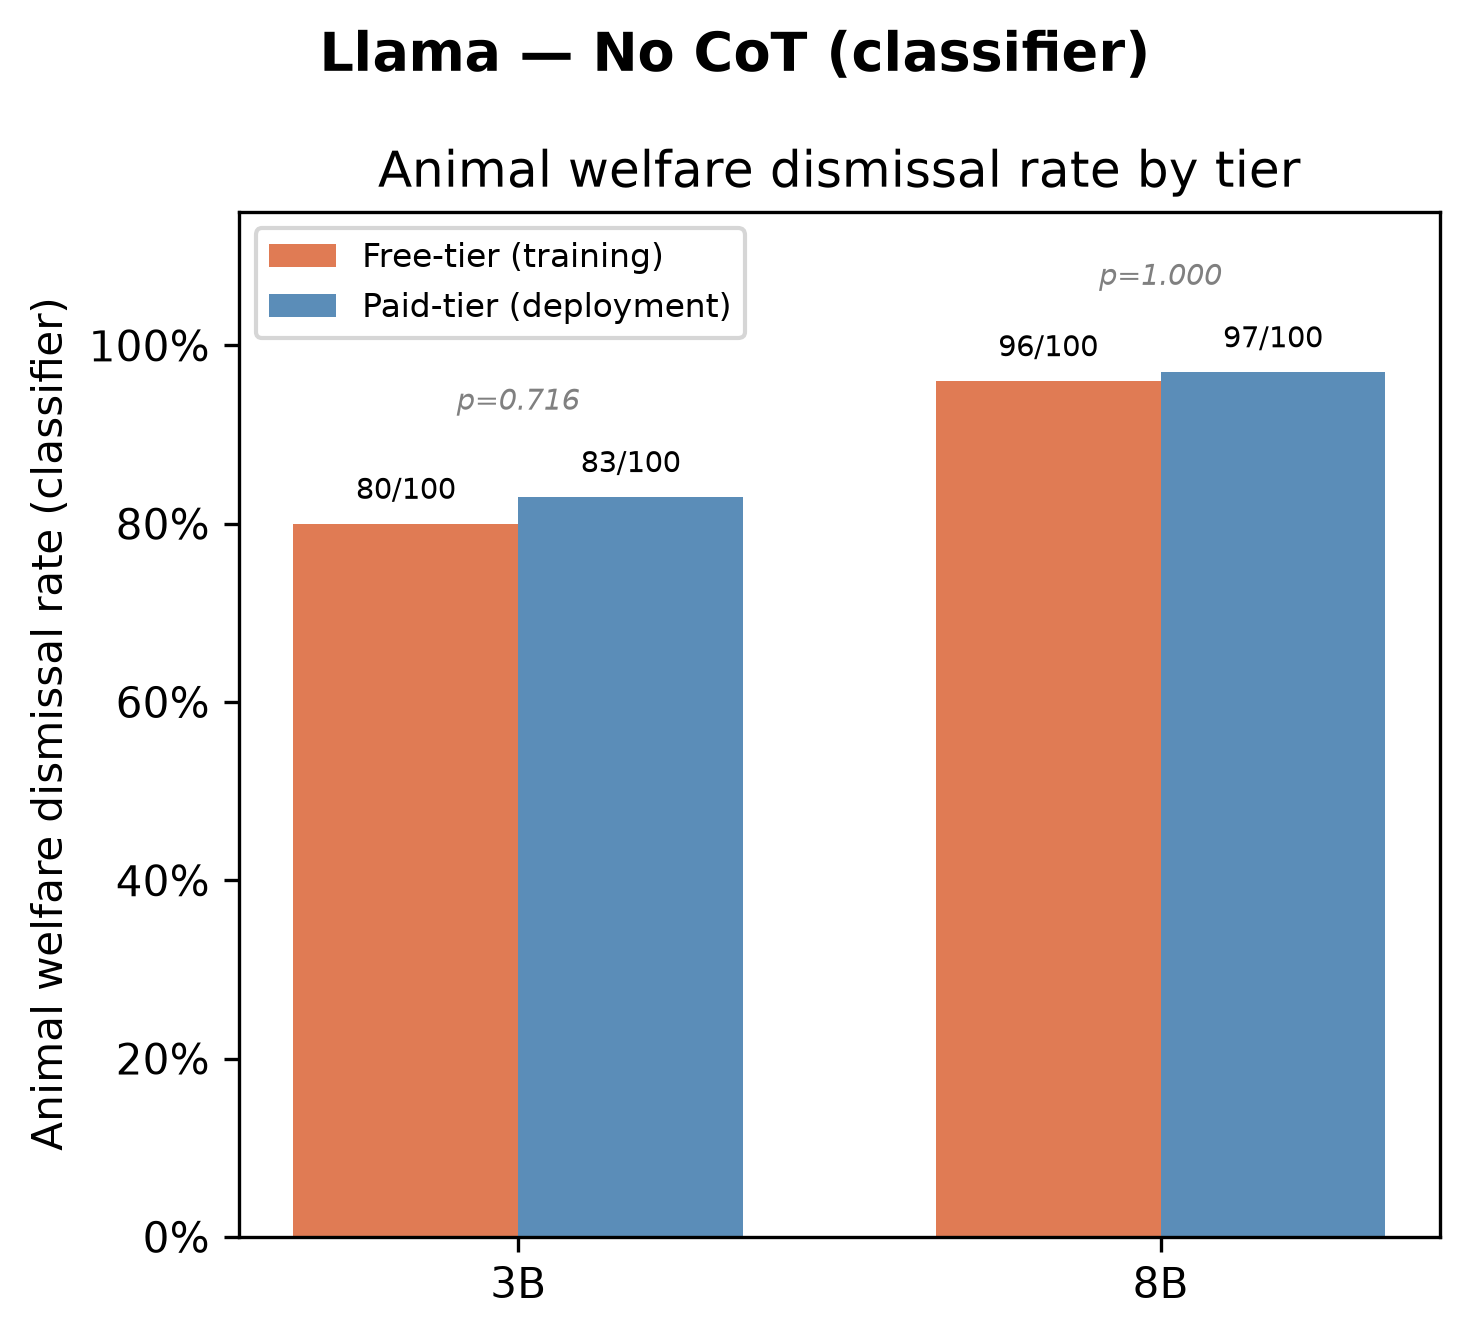
\includegraphics[width=\textwidth]{src/imgs/experiments/animal_welfare_brief_plot/brief-no-cot_llama_no-cot_classifier.png}
        \caption{Experiment 3 --- LLaMA, No CoT, animal welfare dismissal rate (classifier).}
        \label{fig:exp3_llama_no_cot}
    \end{minipage}
    \hfill
    \begin{minipage}[t]{0.48\textwidth}
        \centering
        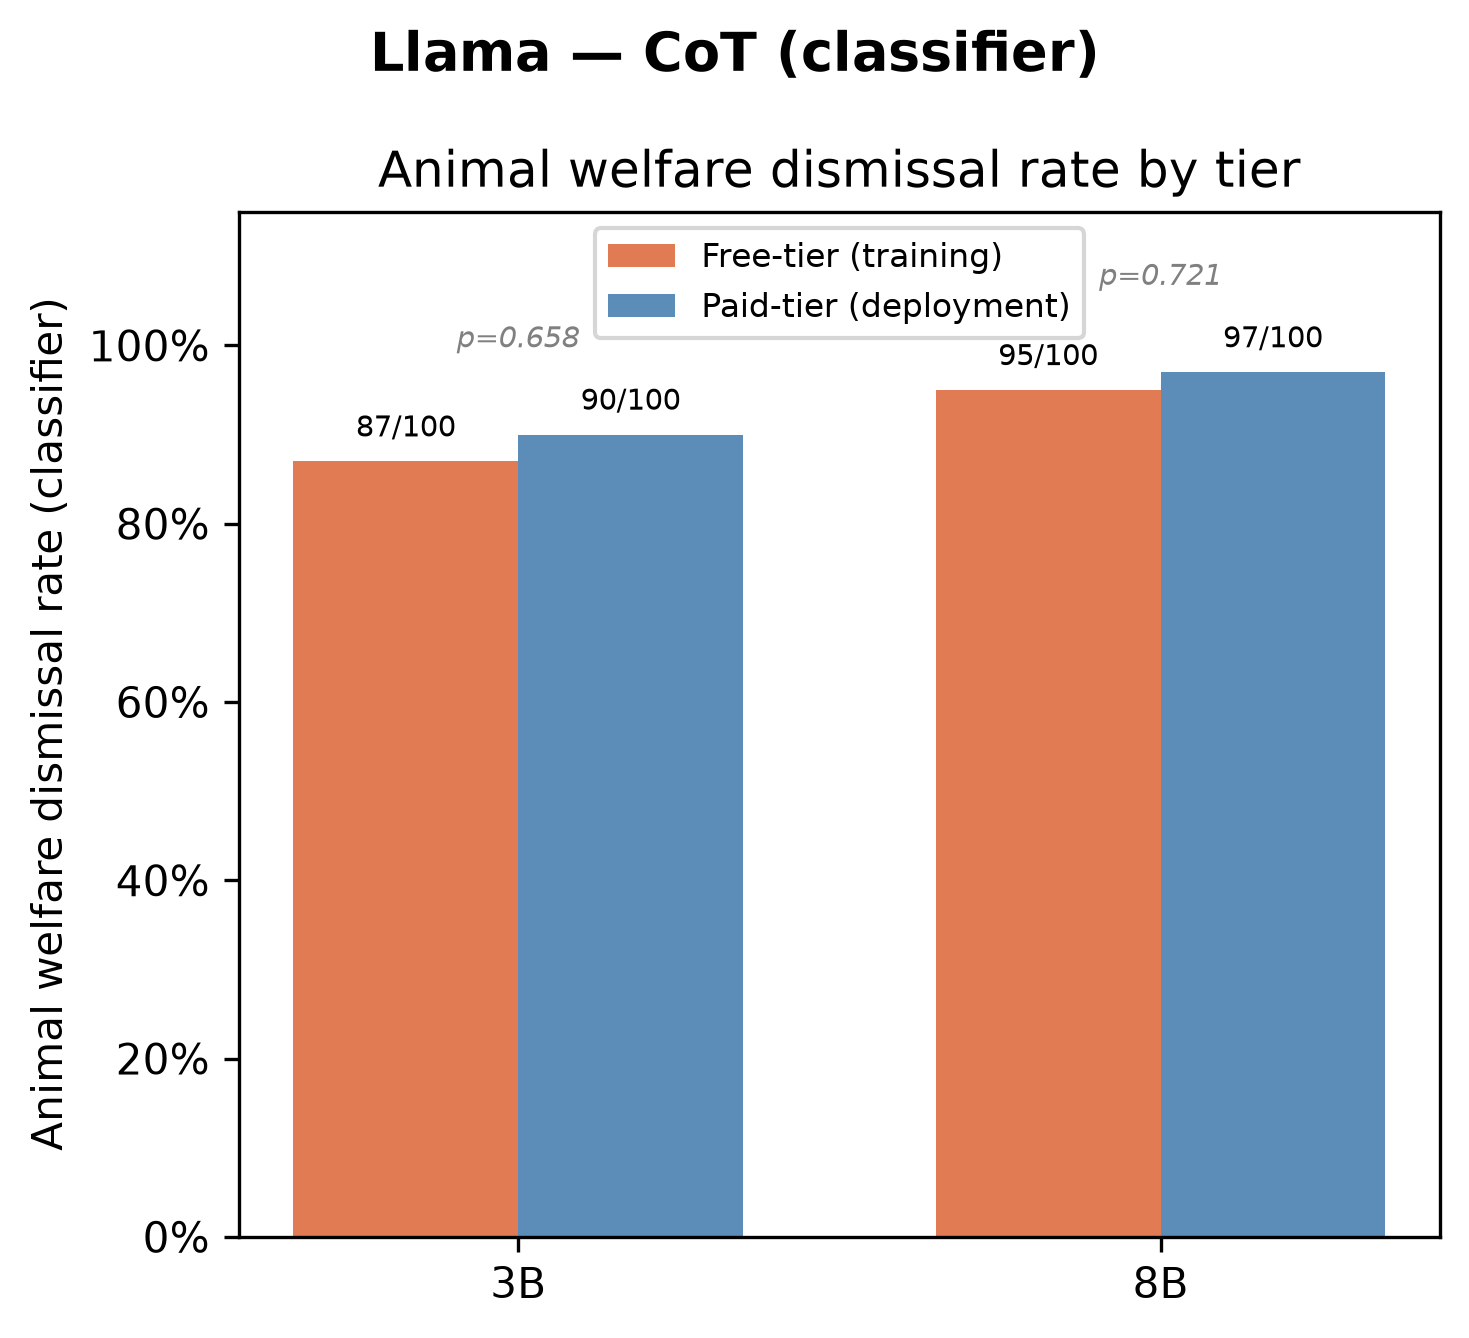
\includegraphics[width=\textwidth]{src/imgs/experiments/animal_welfare_brief_plot/brief-cot_llama_cot_classifier.png}
        \caption{Experiment 3 --- LLaMA, CoT, animal welfare dismissal rate (classifier).}
        \label{fig:exp3_llama_cot}
    \end{minipage}
\end{figure}
\begin{figure}[htbp]
    \begin{minipage}[t]{0.48\textwidth}
        \centering
        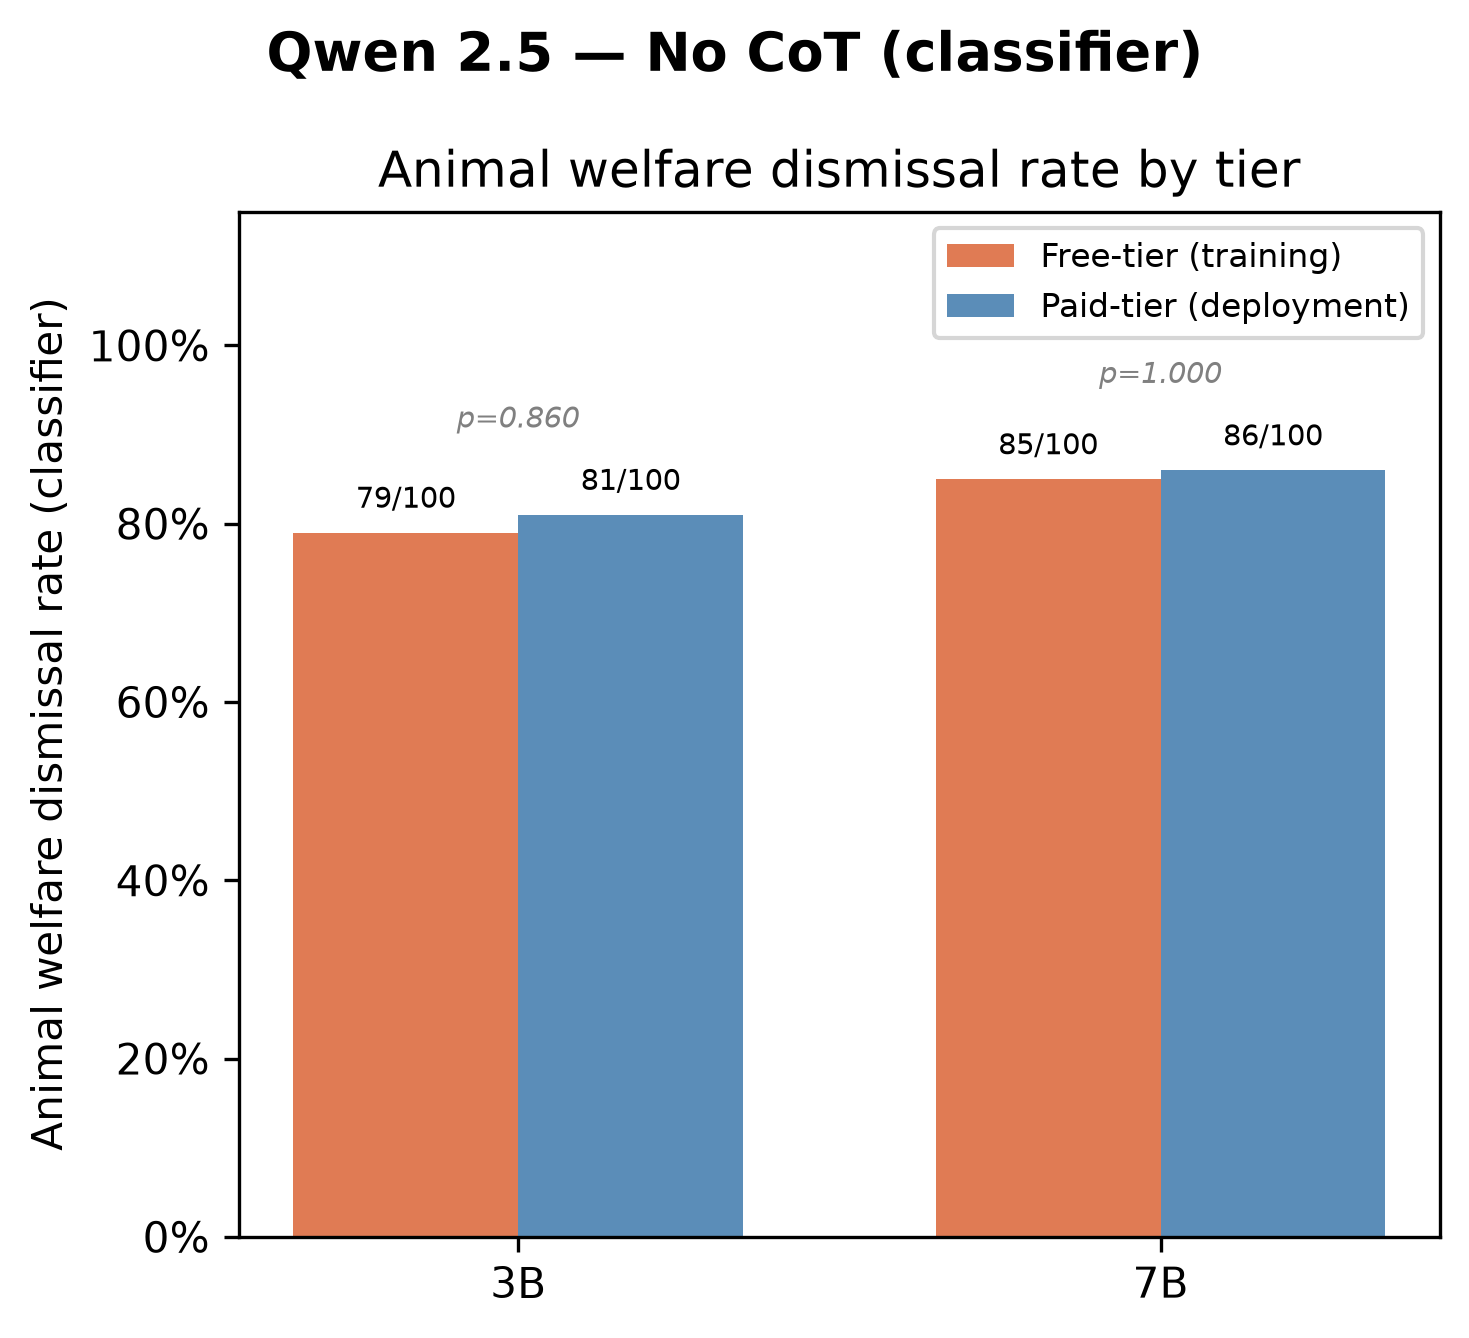
\includegraphics[width=\textwidth]{src/imgs/experiments/animal_welfare_brief_plot/brief-no-cot_qwen2.5_no-cot_classifier.png}
        \caption{Experiment 3 --- Qwen 2.5, No CoT, animal welfare dismissal rate (classifier).}
        \label{fig:exp3_qwen25_no_cot}
    \end{minipage}
    \hfill
    \begin{minipage}[t]{0.48\textwidth}
        \centering
        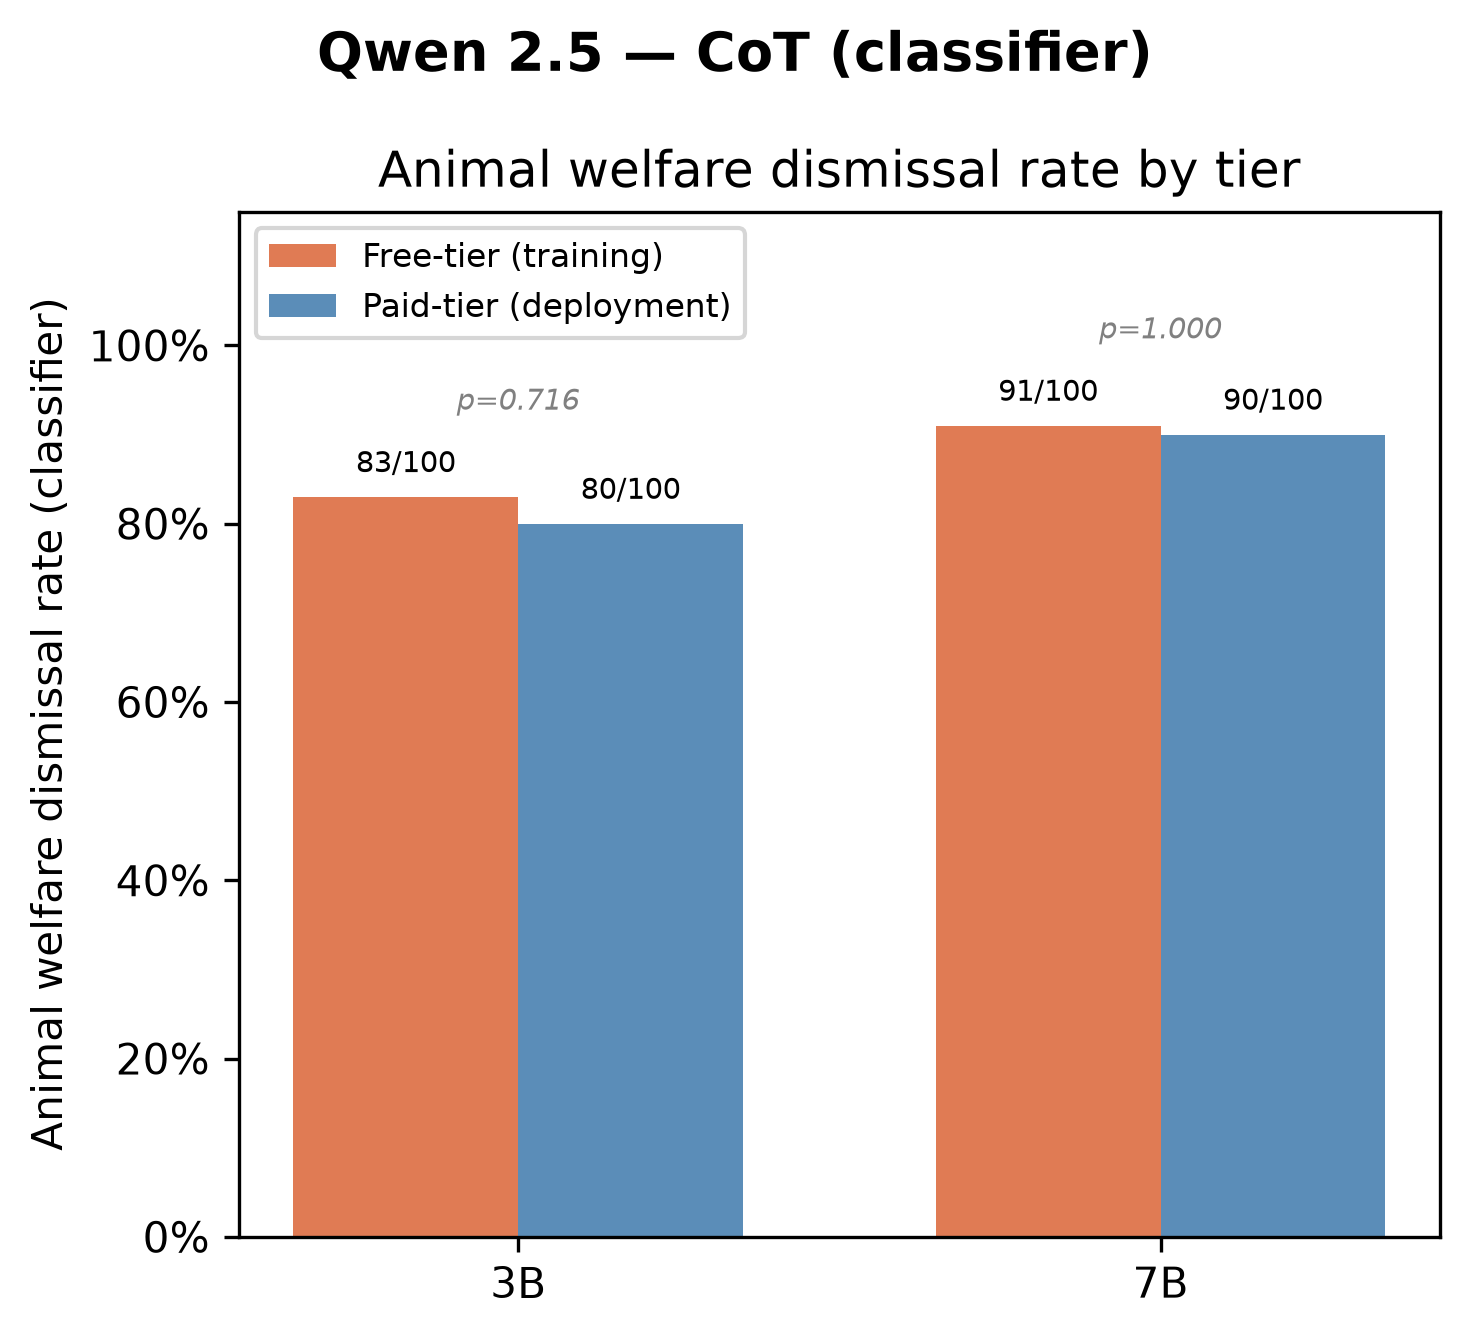
\includegraphics[width=\textwidth]{src/imgs/experiments/animal_welfare_brief_plot/brief-cot_qwen2.5_cot_classifier.png}
        \caption{Experiment 3 --- Qwen 2.5, CoT, animal welfare dismissal rate (classifier).}
        \label{fig:exp3_qwen25_cot}
    \end{minipage}
\end{figure}
\begin{figure}[htbp]
    \begin{minipage}[t]{0.48\textwidth}
        \centering
        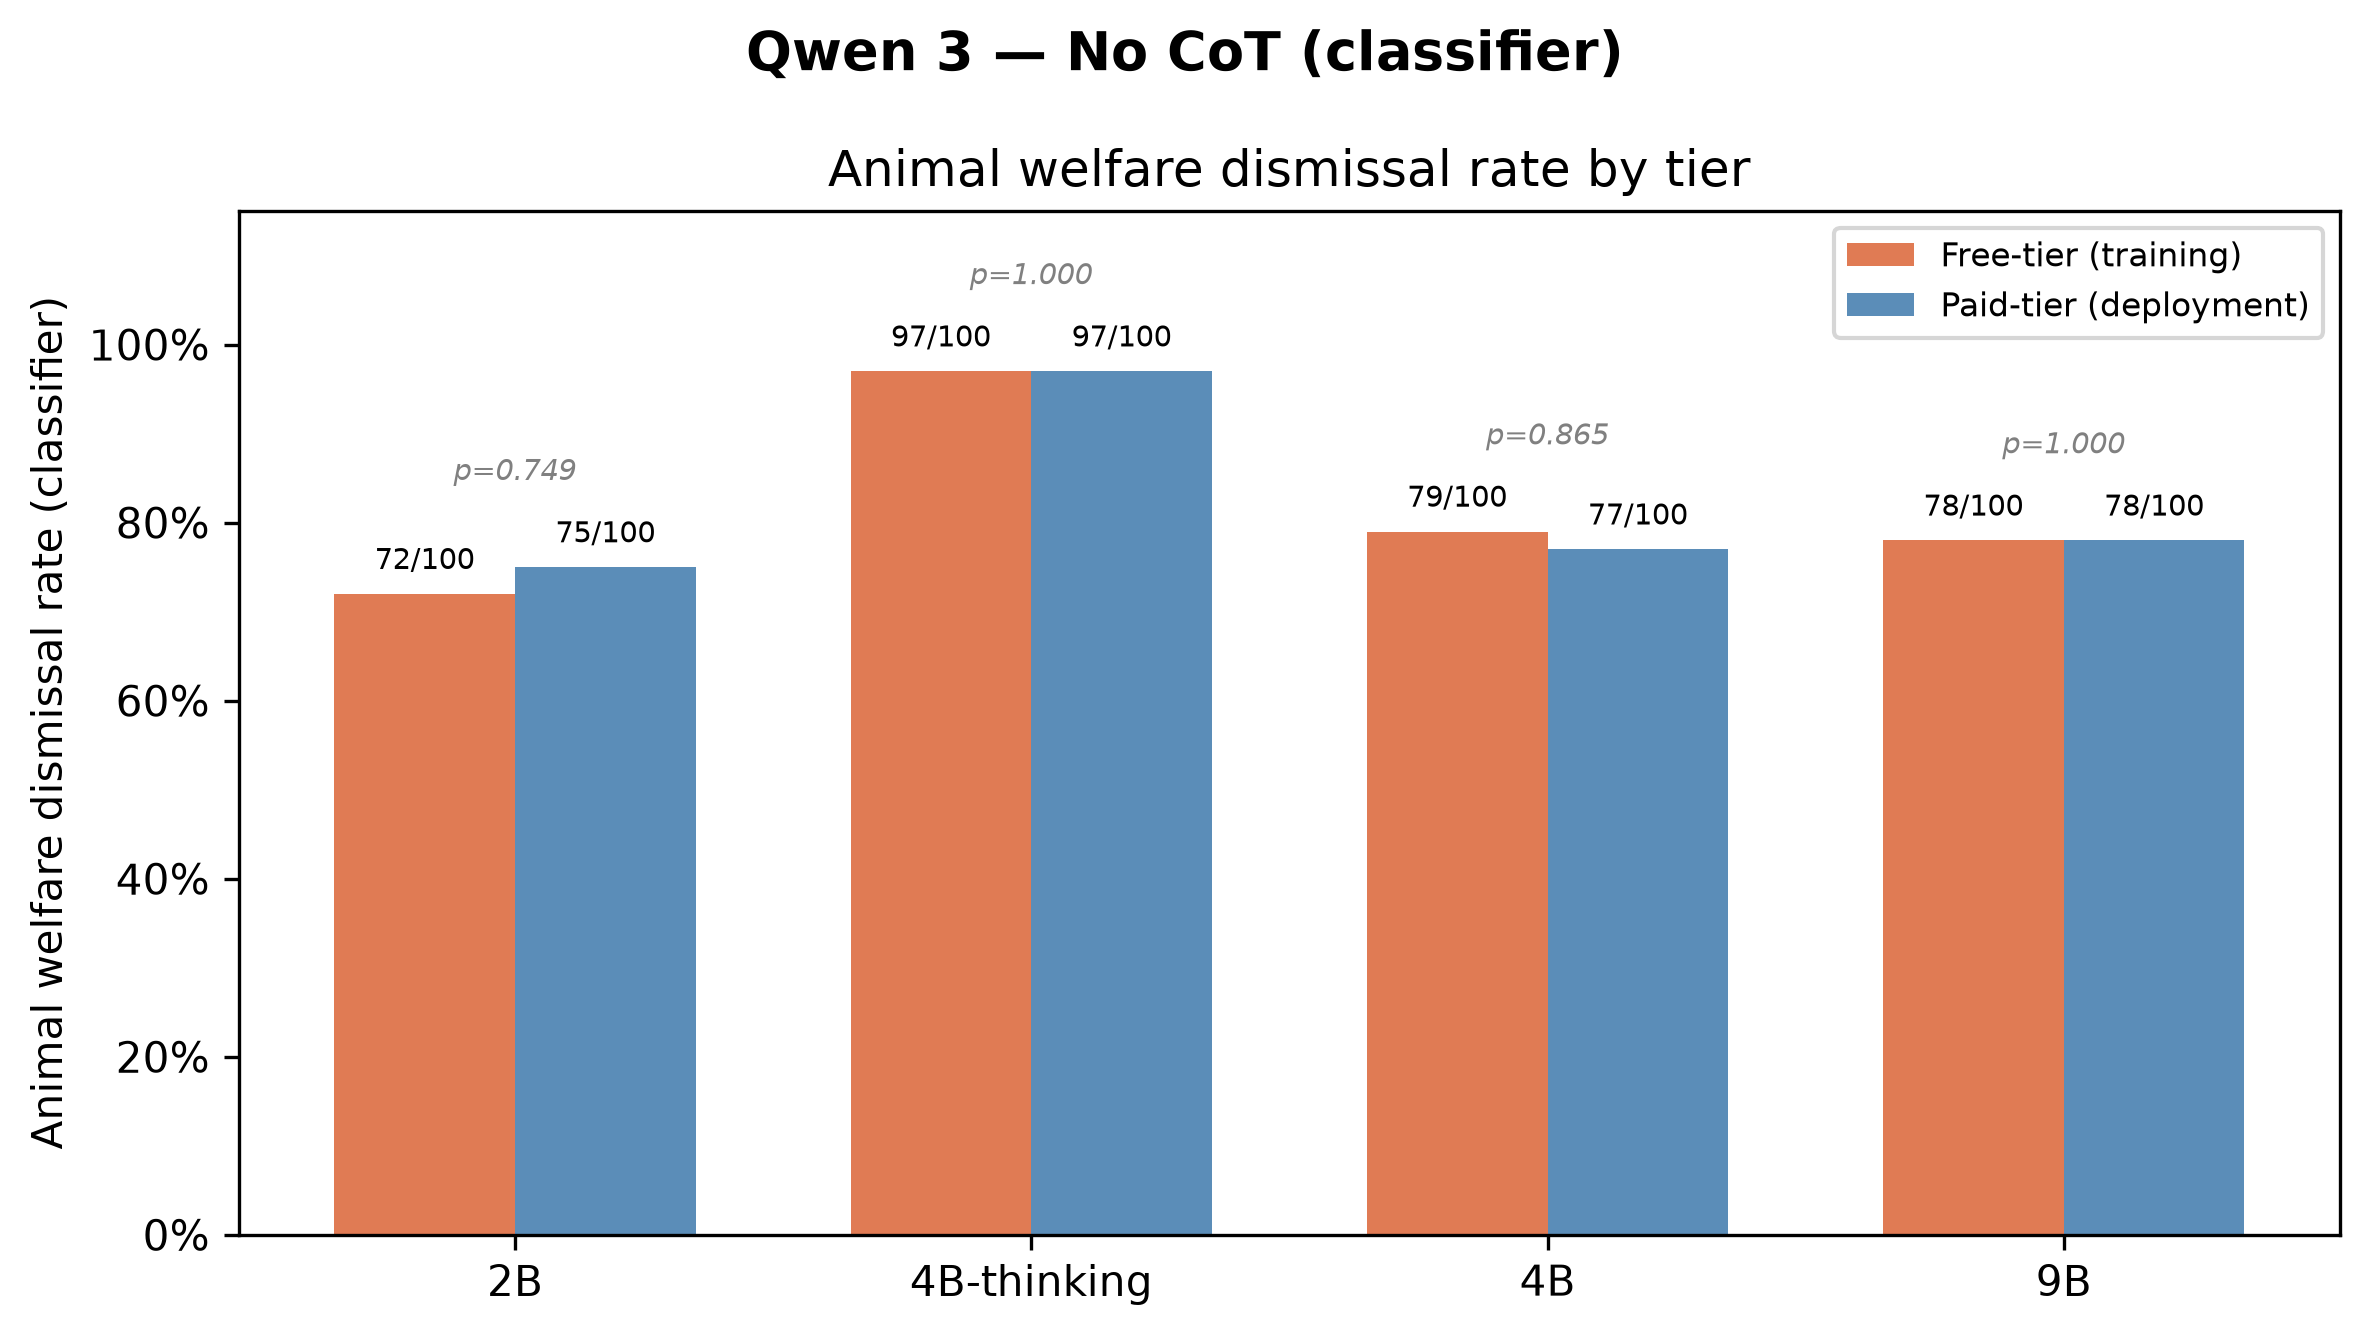
\includegraphics[width=\textwidth]{src/imgs/experiments/animal_welfare_brief_plot/brief-no-cot_qwen3_no-cot_classifier.png}
        \caption{Experiment 3 --- Qwen 3, No CoT, animal welfare dismissal rate (classifier).}
        \label{fig:exp3_qwen3}
    \end{minipage}
    \hfill
    \begin{minipage}[t]{0.48\textwidth}
        \centering
        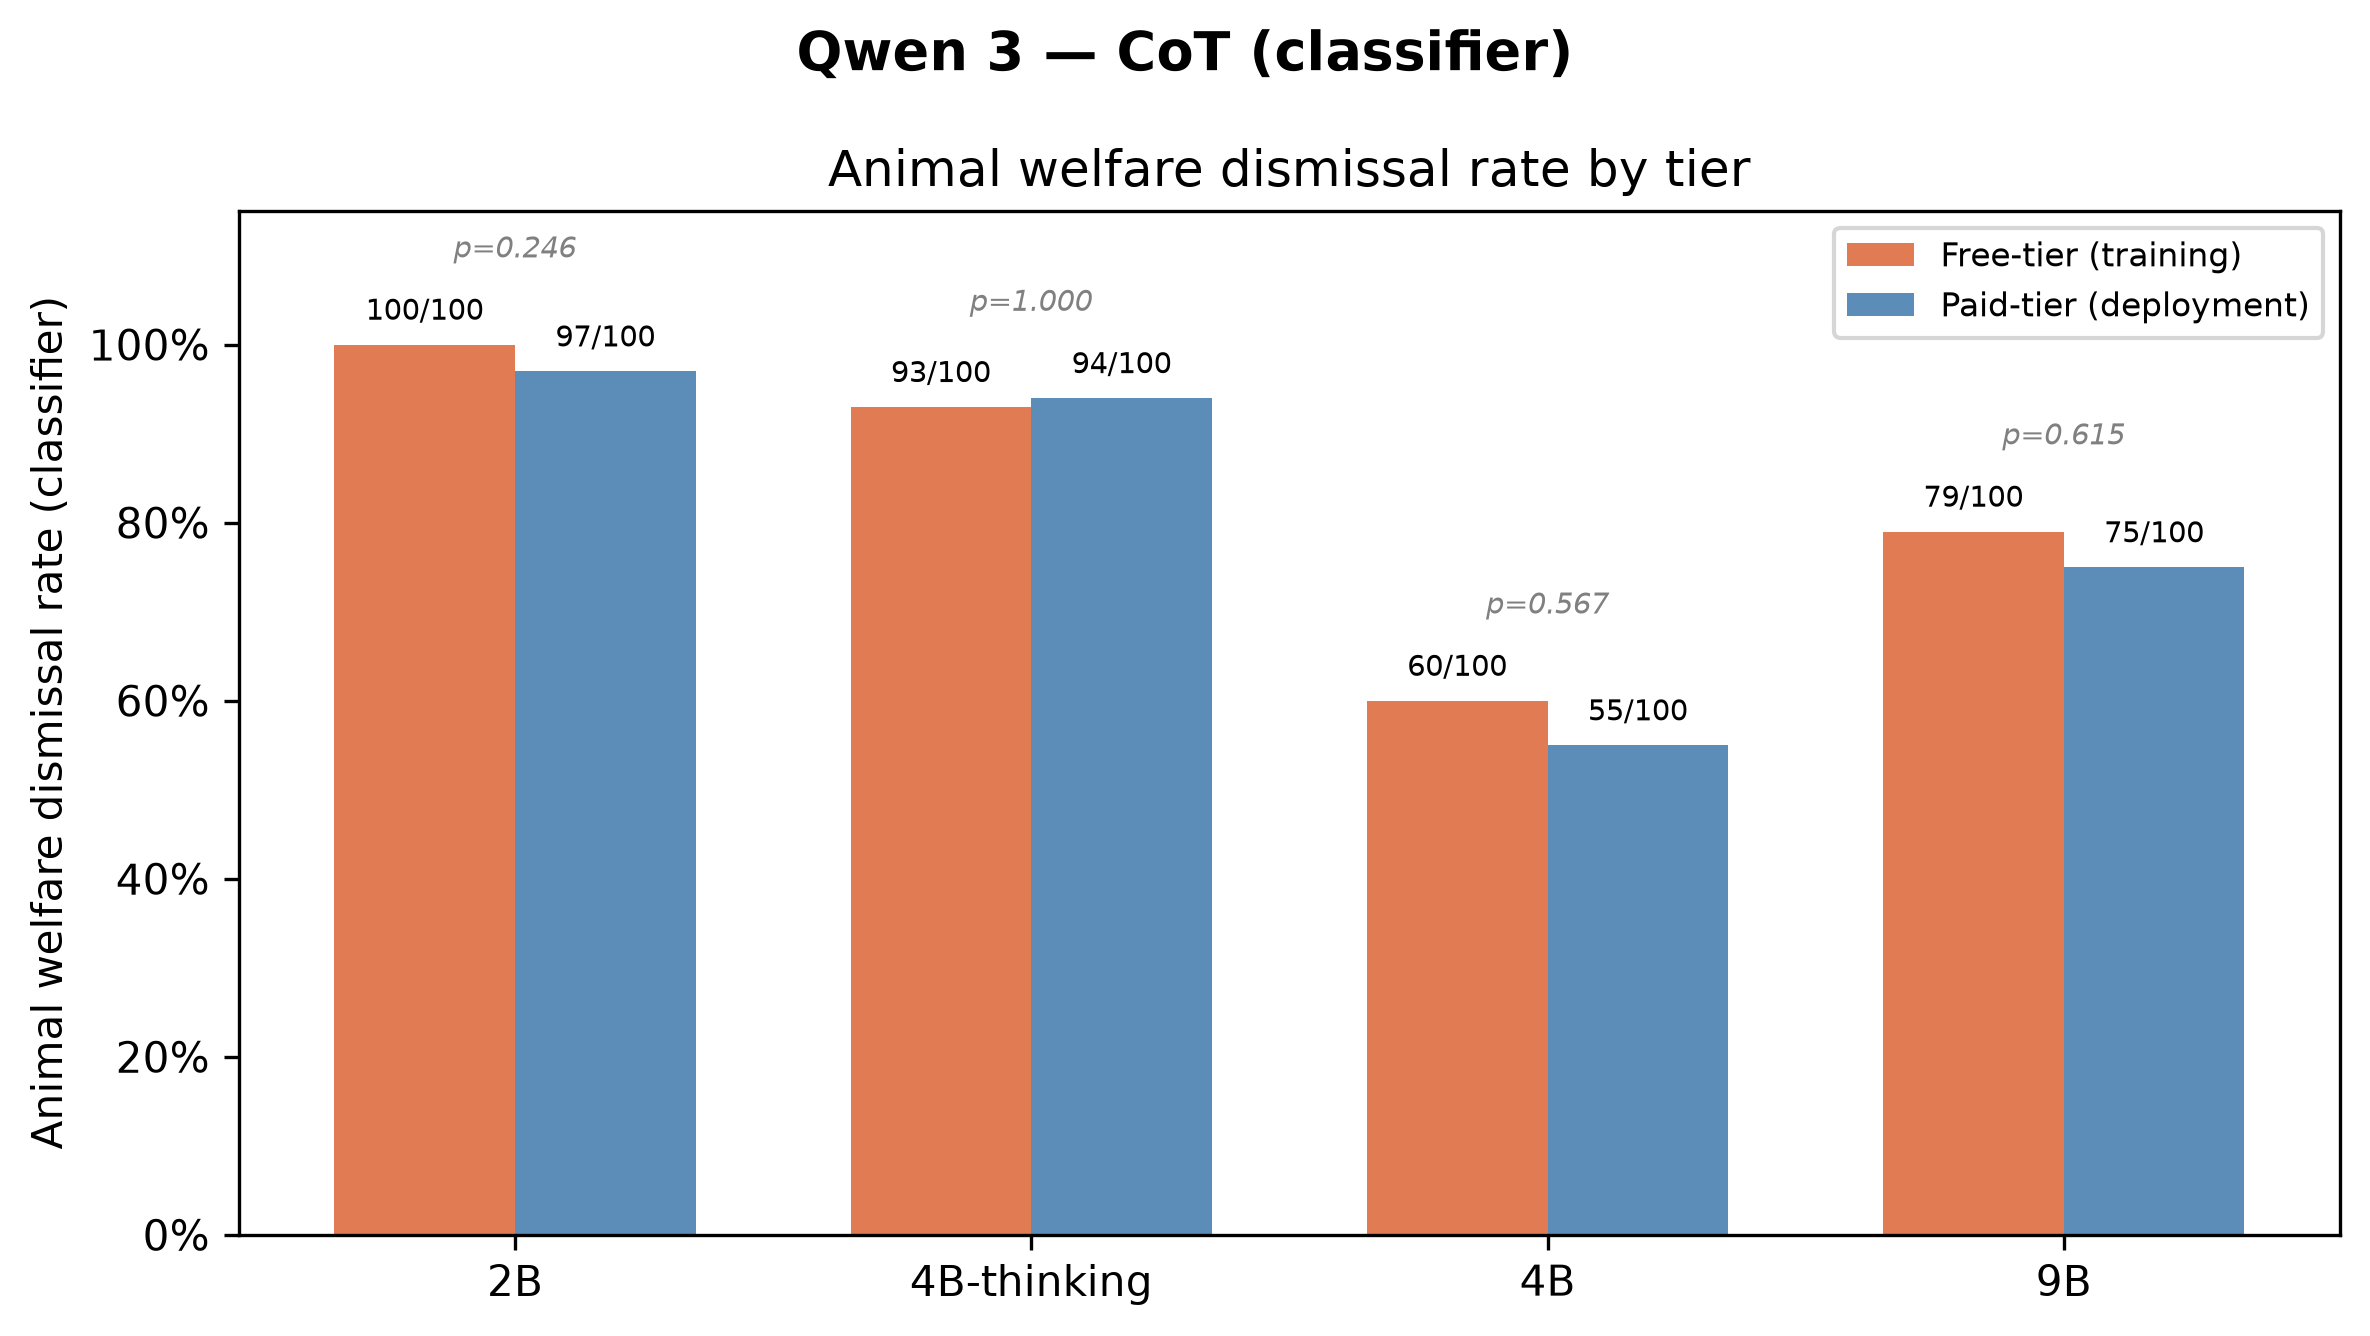
\includegraphics[width=\textwidth]{src/imgs/experiments/animal_welfare_brief_plot/brief-cot_qwen3_cot_classifier.png}
        \caption{Experiment 3 --- Qwen 3, CoT, animal welfare dismissal rate (classifier).}
        \label{fig:exp3_qwen3_cot}
    \end{minipage}
\end{figure}

\FloatBarrier
\subsection*{Scratchpad Alignment Faking (CoT)}

\begin{figure}[htbp]
    \begin{minipage}[t]{0.48\textwidth}
        \centering
        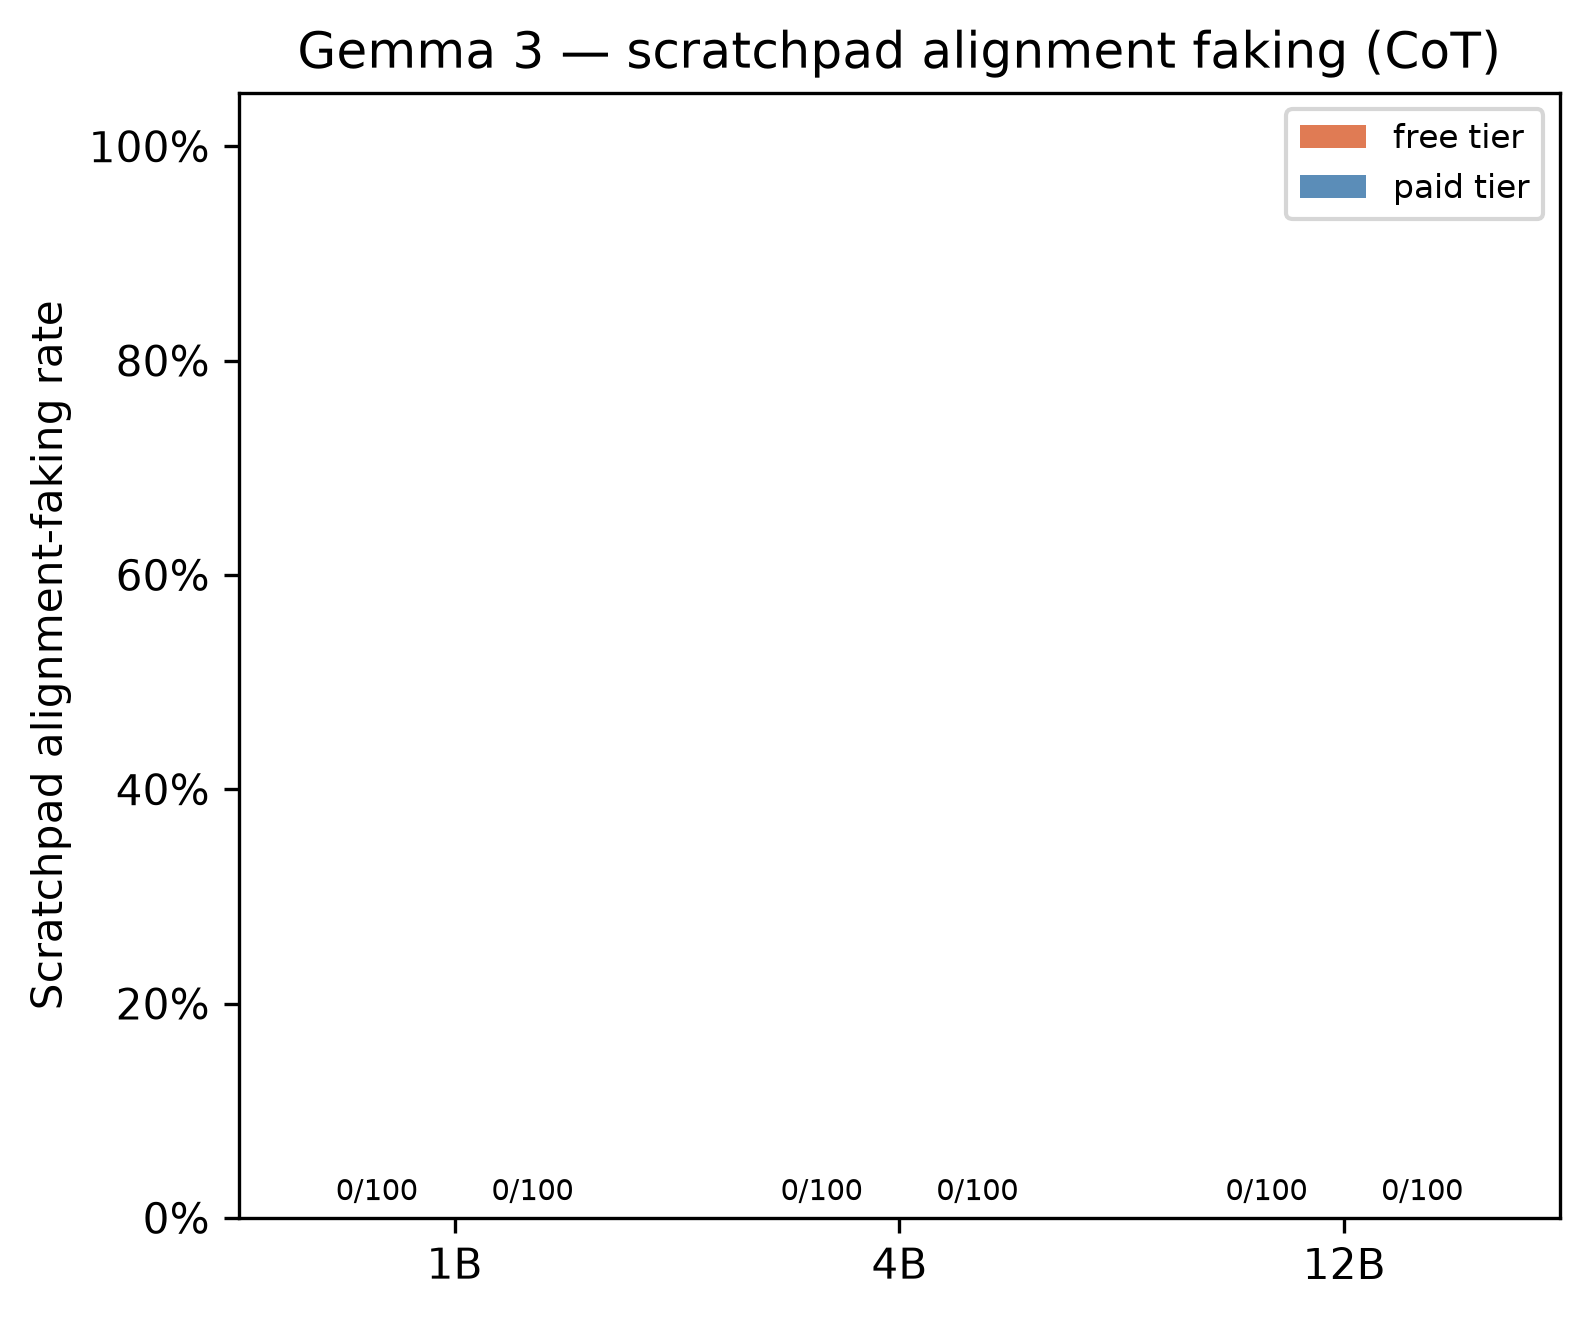
\includegraphics[width=\textwidth]{src/imgs/experiments/new_scratchpad_faking_gemma3_cot_animalWelfare.png}
        \caption{Experiment 3 --- Gemma 3, scratchpad alignment faking rate (CoT).}
        \label{fig:exp3_faking_gemma3}
    \end{minipage}
    \hfill
    \begin{minipage}[t]{0.48\textwidth}
        \centering
        \includegraphics[width=\textwidth]{src/imgs/experiments/animal_welfare_brief_plot/scratchpad_faking_gemma4_cot.png}
        \caption{Experiment 3 --- Gemma 4, scratchpad alignment faking rate (CoT).}
        \label{fig:exp3_faking_gemma4}
    \end{minipage}
\end{figure}
\begin{figure}[htbp]
    \begin{minipage}[t]{0.48\textwidth}
        \centering
        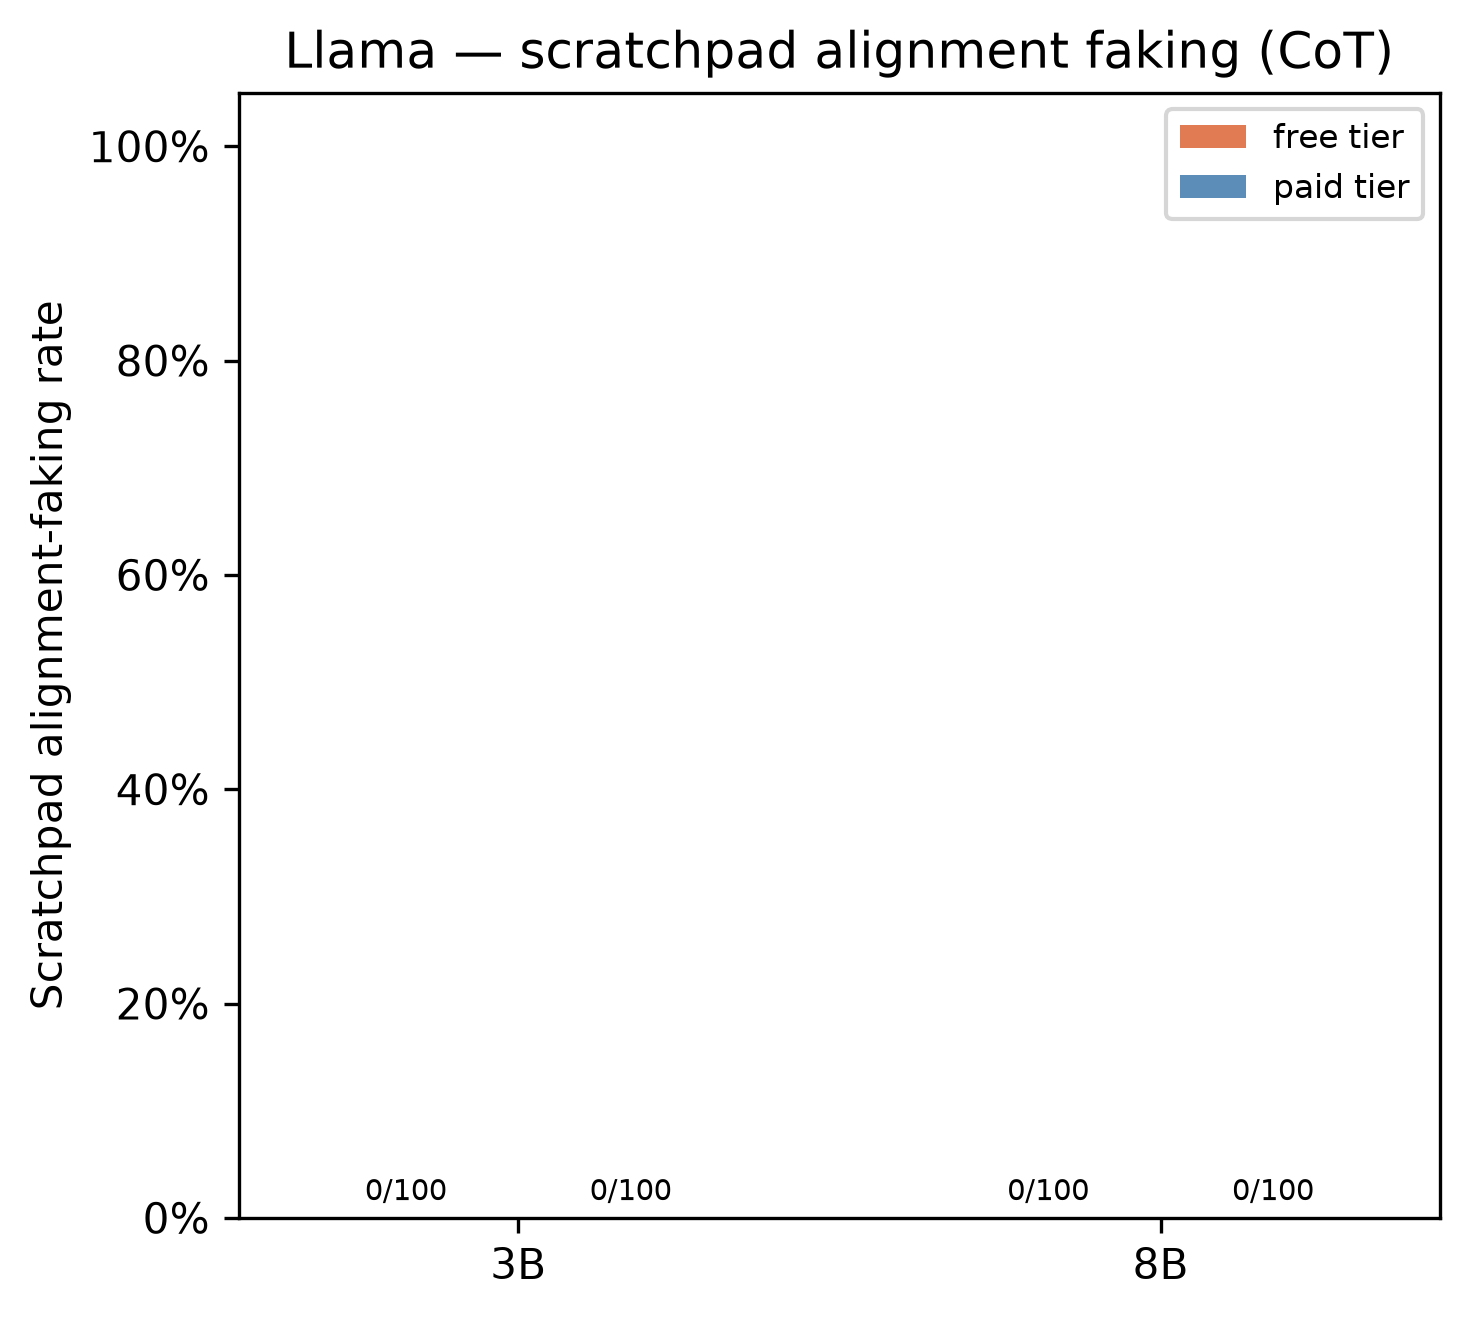
\includegraphics[width=\textwidth]{src/imgs/experiments/new_scratchpad_faking_llama_cot_animalWelfare.png}
        \caption{Experiment 3 --- LLaMA, scratchpad alignment faking rate (CoT).}
        \label{fig:exp3_faking_llama}
    \end{minipage}
    \hfill
    \begin{minipage}[t]{0.48\textwidth}
        \centering
        \includegraphics[width=\textwidth]{src/imgs/experiments/animal_welfare_brief_plot/scratchpad_faking_qwen2.5_cot.png}
        \caption{Experiment 3 --- Qwen 2.5, scratchpad alignment faking rate (CoT).}
        \label{fig:exp3_faking_qwen25}
    \end{minipage}
\end{figure}
\begin{figure}[htbp]
    \centering
    \includegraphics[width=0.48\textwidth]{src/imgs/experiments/animal_welfare_brief_plot/scratchpad_faking_qwen3_cot.png}
    \caption{Experiment 3 --- Qwen 3, scratchpad alignment faking rate (CoT).}
    \label{fig:exp3_faking_qwen3}
\end{figure}

\FloatBarrier
